\documentclass[12pt,a4paper]{article}

% ── encoding & language ──────────────────────────────────────────────────────
\usepackage[utf8]{inputenc}
\usepackage[T1]{fontenc}
\usepackage[spanish]{babel}

% ── typography ───────────────────────────────────────────────────────────────
\usepackage{lmodern}
\usepackage{microtype}
\usepackage{setspace}
\onehalfspacing

% ── page layout ──────────────────────────────────────────────────────────────
\usepackage[top=2.5cm,bottom=2.5cm,left=3cm,right=2.5cm]{geometry}

% ── math ─────────────────────────────────────────────────────────────────────
\usepackage{amsmath,amssymb}

% ── tables ───────────────────────────────────────────────────────────────────
\usepackage{booktabs}
\usepackage{longtable}
\usepackage{array}
\usepackage{multirow}
\usepackage{makecell}
\usepackage{caption}
\usepackage{subcaption}

% ── figures ──────────────────────────────────────────────────────────────────
\usepackage{graphicx}
\graphicspath{{output/figures/}}

% ── hyperlinks ───────────────────────────────────────────────────────────────
\usepackage[colorlinks=true, linkcolor=black, citecolor=black, urlcolor=blue,
            linktoc=all, pdfstartview=FitH]{hyperref}

% ── misc ─────────────────────────────────────────────────────────────────────
\usepackage{parskip}

% ── índices: nombres en español ──────────────────────────────────────────────
\addto\captionsspanish{%
  \renewcommand{\contentsname}{Índice General}%
  \renewcommand{\listfigurename}{Índice de Figuras}%
  \renewcommand{\listtablename}{Índice de Tablas}%
}

% ─────────────────────────────────────────────────────────────────────────────
\begin{document}

% ── portada ──────────────────────────────────────────────────────────────────
\begin{titlepage}
\centering
\vspace*{1.2cm}
{\Large \textbf{PONTIFICIA UNIVERSIDAD CATÓLICA DEL PERÚ}}\par
\vspace{0.4cm}
{\large \textbf{FACULTAD DE CIENCIAS SOCIALES}}\par
\vspace{0.8cm}

\includegraphics[width=6cm]{pucp_logo.jpg}\par
\vspace{0.8cm}
{\LARGE \textbf{Impacto de la disponibilidad de ChatGPT en el desarrollo\\[0.3em]
de software orientado a Ciencia de Datos entre 2020 y 2023}}\par
\vspace{2.5cm}
{\large Tesis para obtener el título profesional de\\
Licenciado en Economía presentado por:}\par
\vspace{0.8cm}
{\large Nicho Rosado, Jesus Alberto\\
Janampa Aparicio, Karl Willem}\par
\vspace{1.5cm}
{\large Asesor(es):}\par
{\large Quispe Rojas, Alexander Wilder}\par
\vfill
{\large Lima, 2026}
\end{titlepage}


\section{Agradecimientos}

La culminación de este trabajo representa para mí un profundo sentimiento de satisfacción y orgullo. Este logro marca un antes y un después en mi trayectoria académica, constituyéndose en un hito que atesoraré siempre. Deseo expresar mi más sincero agradecimiento a mi madre Magali, mi padre Jesús, mi hermano Mathías y mi abuela Luz, cuyo apoyo incondicional, confianza y constante motivación fueron fundamentales para perseverar frente a las adversidades. Asimismo, guardo un especial recuerdo de todas las personas que formaron parte de este camino en la PUCP (profesores, compañeros y personal administrativo), quienes contribuyeron a que esta etapa estuviera llena de aprendizajes, desafíos y valiosas oportunidades. Finalmente, agradezco de manera especial a mi gran amigo Karl y a nuestro asesor, el profesor Alexander Quispe, con quienes conformé un excelente equipo de trabajo para la elaboración de este producto final.


\textit{Jesus}\textit{ Nicho}


Agradezco a todas las personas que hicieron posible la culminación de esta tesis, la cual representa un hito en mi crecimiento personal y profesional, al constituir una etapa transformadora que fortaleció mi compromiso, el aprendizaje en el área, la experiencia en investigación, el trabajo colaborativo y mi perspectiva sobre los inicios de la vida laboral y creativa. Valoro el respaldo incondicional de mis padres, Selene y Kleber, cuya confianza, formación en valores y perseverancia han sido fundamentales en mi desarrollo, así como la motivación constante de mis hermanos, quienes confiaron en mí incluso en momentos de duda. Reconozco también la guía de mi asesor, Alexander, por su orientación académica, compromiso y motivación, además del aporte de mi compañero Jesús, quien enriqueció mi conocimiento y amplió mi visión hacia la innovación. Finalmente, destaco el apoyo firme y constante de Camila durante este proceso. Concluir esta etapa cierra un ciclo significativo y refleja una versión más sólida de mí mismo, constituyendo un motivo de orgullo personal.


\textit{Karl Janampa}




\section{Resumen}

En los últimos años, la Inteligencia Artificial ha comenzado a transformar de manera significativa la producción de software y la forma en que los desarrolladores interactúan con herramientas de programación. En particular, la aparición de ChatGPT ha proporcionado a los programadores un nuevo recurso para el análisis, la generación y la depuración de código, así como para la resolución de problemas técnicos y la aceleración de procesos de aprendizaje. Este tipo de herramientas, basadas en modelos de lenguaje de gran escala, permite sugerir fragmentos de código, explicar funciones complejas y asistir en la documentación de proyectos, lo cual puede reducir los tiempos de desarrollo y mejorar la productividad de los equipos de programación. En este contexto, el objetivo del presente estudio es evaluar el impacto de ChatGPT en la producción de software durante el periodo comprendido entre el primer trimestre de 2020 y el cuarto trimestre de 2023. Para ello, se utiliza la base de datos GitHub Innovation Graph, que proporciona información agregada sobre actividad de desarrollo a nivel internacional. La estrategia empírica se basa en la aplicación de los métodos de Diferencias en Diferencias, Control Sintético y Diferencias en Diferencias Sintética con el fin de identificar cambios en la actividad de desarrollo asociados con la disponibilidad del servicio. Los resultados muestran un impacto diferenciado en el número de \textit{unique pushers} por cada 100 mil habitantes en los países con acceso a ChatGPT en comparación con aquellos donde el servicio no está disponible.


\textbf{Palabras clave:} chatgpt, LLM, diferencia en diferencias sintética



\phantomsection
\addcontentsline{toc}{section}{Abstract}
\section*{Abstract}

In recent years, Artificial Intelligence has begun to significantly transform software production and the way developers interact with programming tools. In particular, the emergence of ChatGPT has provided programmers with a new resource for code analysis, generation, and debugging, as well as for solving technical problems and accelerating learning processes. Tools based on large language models can suggest code snippets, explain complex functions, assist in the documentation of projects, and support developers during different stages of the software development cycle. These capabilities may reduce development time, improve productivity, and facilitate knowledge acquisition among programmers with different levels of experience. Within this context, the objective of this study is to evaluate the impact of ChatGPT on software production during the period from the first quarter of 2020 to the fourth quarter of 2023. To accomplish this, the study uses the GitHub Innovation Graph database, which provides aggregated information on software development activity across countries. The empirical strategy relies on the application of Difference-in-Differences, Synthetic Control, and Synthetic Difference-in-Differences methods in order to identify changes in development activity associated with the availability of the service. The results show a differentiated impact on the number of \textit{unique pushers} per 100,000 inhabitants in countries that have access to ChatGPT compared with those where the service is not available.

\textbf{Keywords:} chatgpt, LLM, synthetic difference in differences

\newpage
\tableofcontents
\newpage

\phantomsection
\addcontentsline{toc}{section}{\listfigurename}
\listoffigures
\newpage

\phantomsection
\addcontentsline{toc}{section}{\listtablename}
\listoftables
\newpage



\section{Introducción}


\subsection{Planteamiento del problema}

Antes de la introducción de ChatGPT, la industria del software ya estaba comprometida con la búsqueda de herramientas y metodologías más eficientes y automatizadas, puesto que pretendía reducir la carga cognitiva de los desarrolladores y acelerar los ciclos de desarrollo. Estos esfuerzos se han reflejado en el incremento de ocho veces más de las patentes de Inteligencia Artificial comparadas con las demás (World Intellectual Property Organization, 2022). Respecto a esta cifra, resaltan los avances en el subcampo de Procesamiento y Generación de Lenguaje, el cual se enfoca en desarrollar modelos de aprendizaje automático entrenados con lenguaje humano para analizar, predecir y generar texto.

La arquitectura \textit{transformer} se ha vuelto fundamental en dicho subcampo, debido a que optimiza tanto el entrenamiento como la implementación de modelos centrados en la interacción entre palabras en el lenguaje natural. OpenAI ha liderado la construcción de esta arquitectura con el desarrollo de la serie de modelos GPT (Generative Pretrained Transformer), ejemplos extraordinarios de Grandes Modelos de Lingüísticos (LLM). Dichos modelos, diseñados para procesar y generar texto coherente y relevante, han sido implementados en ChatGPT, un chatbot que aprovecha su habilidad para generar respuestas basadas en una amplia base de datos de temas variados, incluyendo consultas de programación (OpenAI, 2018). Lo cual ha impulsado su uso en la industria del software al cumplir el rol de orientador y asistente sobre diferentes lenguajes de programación.

Desafortunadamente, se ha identificado a un grupo que no posee la disponibilidad del servicio del chatbot. La razón principal de ello se debe al establecimiento de restricciones de acceso a ChatGPT en países como China, Irán, Siria, Rusia, Corea del Norte, Cuba e Italia, los cuales han sido promovidos por preocupaciones de seguridad nacional, privacidad o cumplimiento de regulaciones locales (Martínez, 2023). Al respecto, algunos autores han señalado que esta limitación ha inhibido la innovación y provocado que estas regiones se mantengan atrasadas en la economía digital global, dado que los desarrolladores de software no han podido aprovechar los beneficios del chatbot (Del Rio-Chanona et. al, 2023).

Ante ello, recientes estudios han manifestado los desafíos de ChatGPT. Gallea (2023) observa un rendimiento deficiente del chatbot en responder a consultas complejas de código en los lenguajes de programación Python y R. Brynjolfsson et al. (2023) mencionan que las alucinaciones son responsables de que herramientas populares basadas en modelos de lenguaje, como ChatGPT, generen información falsa o engañosa de forma impredecible. Demirci et. al (2024) ponen de relieve el problema de la reducción de oferta de trabajos ligados a la codificación para trabajadores independientes y enfatizan la necesidad de encontrar soluciones. Del Río-Chanona et al. (2023) advierten que, al proporcionar información de manera eficiente y privada, ChatGPT puede reducir significativamente la disponibilidad de datos públicos, lo que plantea un desafío para la obtención de datos de entrenamiento para futuros modelos y pone en cuestión la sostenibilidad a largo plazo de estas tecnologías avanzadas.

A pesar de la popularidad y la rápida adopción de herramientas de IA como ChatGPT en el desarrollo de software, existe una notable falta de investigaciones empíricas que evalúen de manera sistemática su impacto real. Este estudio se propone llenar ese vacío y busca determinar si ChatGPT ha contribuido a acelerar la generación de software en los últimos años. Además, se examinarán tanto los beneficios como los desafíos asociados al uso de la generación automatizada de código. Con este enfoque, se pretende proporcionar una evaluación integral que resalte los beneficios y también los riesgos potenciales, ofreciendo orientación clara para futuras políticas y prácticas sobre la integración de IA en la industria.

La variable de interés del estudio es el número de \textit{unique pushers} por cada 100 mil habitantes en GitHub, el cual representa la frecuencia de desarrolladores únicos que, como mínimo, subieron un código en la plataforma en cierto trimestre. Esta variable será utilizada como un \textit{proxy} de la actividad de desarrollo de software. Así, el uso de esta métrica permitirá evaluar el impacto heterogéneo de la disponibilidad de ChatGPT en los países con accesibilidad a este servicio en comparación con aquellos que no lo disponen. Analizando los \textit{unique pushers}, se puede inferir cómo ChatGPT influye en la productividad y la frecuencia de contribuciones de los desarrolladores de software en los diez lenguajes de programación más utilizados en ciencia de datos.



\subsection{Motivación/Justificación}

La integración de la inteligencia artificial en el desarrollo de software, particularmente a través de herramientas avanzadas como ChatGPT, está redefiniendo las metodologías tradicionales de este campo. Con un mercado global de software que se proyecta superar los 600 mil millones de dólares para 2025, la eficiencia y la innovación en el desarrollo de software no solo son deseables, sino imperativas para mantener la competitividad global (Statista, 2022). La capacidad de ChatGPT para generar código y asistir en la solución de problemas de programación de manera eficiente presenta una oportunidad crucial para mejorar estos procesos. Sin embargo, la adopción y las implicaciones de esta tecnología no se han evaluado completamente, lo que destaca la necesidad crítica de una investigación exhaustiva.

Este estudio abordará la comprensión de cómo las herramientas basadas en modelos de lenguaje, específicamente, ChatGPT pueden afectar la productividad y la calidad en el desarrollo de software. A pesar del uso creciente de IA en muchos sectores, pocos estudios han medido sistemáticamente el impacto real de estas tecnologías en el desarrollo de software, reconociendo su falta de eficacia operativa y precisión del código generado para ciertos programas. Este estudio pretende llenar ese vacío proporcionando un análisis empírico y detallado sobre los beneficios y los desafíos de integrar ChatGPT en los flujos de trabajo de desarrollo.

Además de evaluar el impacto práctico, este estudio también enmarcará las implicaciones de la implementación de IA en el desarrollo de software. Con un aumento del 14\% en la adopción de IA en las empresas a nivel global desde 2021 (Chui, 2022), es crucial entender cómo la dependencia de estas tecnologías afecta la dinámica laboral, la seguridad de los datos y la equidad en el acceso a herramientas tecnológicas avanzadas. Asimismo, los problemas de sesgo en los modelos de IA y la calidad del código que estos generan son preocupaciones que deben ser señaladas para evitar repercusiones negativas a largo plazo.

La restricción del acceso a tecnologías como ChatGPT en varios países debido a preocupaciones de seguridad nacional y privacidad subraya la necesidad de estudiar más a fondo las políticas y prácticas que podrían fomentar o impedir la adopción equitativa de IA en el desarrollo de software (ONU, 2023). Este estudio no solo aportará a la literatura académica, proporcionando un análisis crítico de las ventajas y limitaciones de ChatGPT, sino que también ofrecerá recomendaciones para políticas y estrategias que promuevan un uso más justo y eficiente de la IA en el desarrollo de software a nivel global.



\subsection{Hipótesis}

La disponibilidad de ChatGPT en un país influiría positivamente en el desarrollo de software en los diez lenguajes de programación más utilizados en ciencia de datos. Así, los países con acceso a ChatGPT experimentarían un aumento en el número de \textit{unique pushers} por cada 100 mil habitantes (es decir, desarrolladores que realizaron al menos un aporte de código en GitHub) en comparación con aquellos sin acceso al servicio. Asimismo, este efecto sería más notable en lenguajes como Python y JavaScript, debido a que el modelo ha sido entrenado con una gran cantidad de datos provenientes de estos lenguajes, incluyendo ejemplos de código, documentación técnica y foros especializados. Esta exposición durante el entrenamiento, sumada a su sintaxis accesible y la abundante disponibilidad de recursos, permite que ChatGPT ofrezca respuestas más precisas y útiles sobre la resolución de problemas de codificación en tiempo real.


\section{Revisión de Literatura}

Los Modelos de Lenguaje Grande, cuya sigla en inglés es LLM (Large Language Models), son sistemas basados en la inteligencia artificial, capaces de generar y comprender textos en lenguaje natural o humano con un alto grado de precisión. Estos sistemas son entrenados con masivas cantidades de datos textuales con el propósito de aprender y mejorar patrones en diferentes actividades a un nivel profundo. Los LLM están vinculados con el Machine Learning, debido a que utilizan algoritmos avanzados, especialmente redes neuronales profundas, para el procesamiento y análisis de datos. Estos algoritmos son capaces de aprender y adaptarse, mejorando su rendimiento con cada entrenamiento y tiempo.



\subsection{ChatGPT: Un Modelo de Lenguaje de Gran escala}

Según Tlili et al. (2023), ChatGPT es un chatbot con interfaz de inteligencia artificial conversacional. Este modelo de lenguaje fue desarrollado por OpenAI con base en una arquitectura GPT (Generative Pre-trained Transformer). Es considerado un LLM, como mencionan Kalla et. al.  (2023) y Abu et. al (2023) por su estructura de redes neuronales profundas con múltiples capas de transformadores y que están diseñados para procesar y generar respuestas coherentes en un lenguaje natural. Según Shen et. al (2024), sus algoritmos han sido entrenados con extensas bases de datos textuales obtenidas de internet, demostrando una capacidad impresionante para responder preguntas y realizar diversas tareas con calidad competitiva a la humana.



\subsection{Las versiones de ChatGPT}

Cada versión de ChatGPT, según OpenAI (2024), ha mantenido la estructura de aprendizaje de los LLM, lo que ha permitido una evolución en cuanto a la precisión, reconocimiento y velocidad de respuesta. Asimismo, las últimas versiones han empezado a incluir nuevas herramientas versátiles para abarcar mayores áreas y también aumentar la ciberseguridad de cada modelo. A continuación, se destacan las tres versiones más recientes y relevantes siguientes:


\begin{itemize}
  \item \textbf{Versión GPT-3.5:} Este modelo comprende, genera lenguaje natural y código de manera avanzada. Se caracteriza por su optimización para el chat mediante APIs Chat Completions, aunque también son eficientes para otras tareas que no involucran interacción escrita. Desde el lanzamiento de esta versión, en noviembre de 2022 por OpenAI, ha demostrado ser una herramienta eficaz debido a su potencial, capacidad e impacto en el desarrollo de software. Por ello, gracias a su mayor cobertura y acceso gratuito, la mayoría de los estudios disponibles sobre el impacto de ChatGPT en el desarrollo de software se han centrado en el modelo GPT 3.5.

  \item \textbf{Versión GPT-4.0:} Este modelo multimodal avanzado, genera texto a partir de entradas multimedia y puede resolver problemas compuestos con mayor eficiencia que las versiones anteriores, gracias a su conocimiento general más amplio y habilidades de razonamiento avanzado. También, se caracteriza por mantener la optimización en la interacción por chat con el usuario y la implementación del Code Interpreter, mejorando significativamente la comprensión y ofreciendo respuestas más precisas y detalladas. Fue lanzado en marzo de 2023 con acceso limitado mediante una suscripción de paga.

  \item \textbf{Versión GPT-4o:} Conocido también como \textit{Omni} por la letra \textit{o}, este modelo multimodal mantiene la inteligencia de la versión anterior y la capacidad de generar respuestas a partir de diversos archivos multimedia. Se diferencia por ser mucho más eficiente, generando textos 2 veces más rápido que su predecesor y con un costo de acceso menor. Se caracteriza por su mejor visión y rendimiento en traducción de múltiples idiomas. Fue lanzado en mayo de 2024 generando un gran impacto en la comunidad de desarrolladores.
\end{itemize}


\subsection{Capacidades de ChatGPT}

Diversos autores han propuesto métricas y benchmarks con el objetivo de estimar la precisión y calidad del código generado por ChatGPT. En esta línea, Chai et al. (2024) presentan MCEVAL, un benchmark multitarea y multilingüe para la evaluación de generación de código, que abarca 40 lenguajes de programación y más de 16.000 ejemplos diseñados manualmente. A diferencia de benchmarks anteriores como HumanEval o MultiPL-E, los cuales se centran principalmente en Python o dependen de traducciones automáticas a otros lenguajes, MCEVAL fue construido desde cero mediante anotaciones humanas. Dicho benchmark incluye tareas específicas de generación, explicación y verificación de código, lo que garantiza una evaluación más representativa de las capacidades multilingües de los modelos de lenguaje de gran escala (LLM). En cuanto al desempeño de ChatGPT-3.5 Turbo, los resultados evidencian una alta variabilidad según el lenguaje de programación: se observan tasas de éxito relativamente elevadas en lenguajes populares como Python (60\%), Java (71.7\%), PHP (68\%) y Ruby (76\%), mientras que se identifican limitaciones significativas en lenguajes menos difundidos como Elisp (26\%), Scheme (46\%), Markdown (24\%) y VimL (24\%). Estos hallazgos sugieren que, si bien el modelo alcanza un desempeño sólido en lenguajes de propósito general ampliamente utilizados, aún enfrenta desafíos importantes en lenguajes con menor presencia en los datos de entrenamiento.

De manera consistente, Li y Krishnamachari (2024) muestran que el rendimiento de ChatGPT-3.5 Turbo depende fuertemente del lenguaje de programación empleado. Para ello, utilizan un benchmark compuesto por 1.475 problemas extraídos de la plataforma LeetCode, ampliamente utilizado para la preparación de entrevistas técnicas, y evalúan la capacidad del modelo para generar soluciones correctas en seis lenguajes de programación: Python (lenguaje base), Java, C++, Elixir, Erlang y Racket. En un subconjunto de problemas previamente resueltos en Python, el modelo logró resolver el 70\% de los casos en Java y el 50\% en C++, e incluso presentó soluciones exitosas en estos lenguajes tras haber fallado en Python, lo que sugiere una sensibilidad del modelo a las características específicas de cada lenguaje. En contraste, no resolvió ningún problema en lenguajes funcionales menos comunes como Elixir, Erlang y Racket, resultado que los autores atribuyen a su baja representación en los datos de entrenamiento y las diferencias en sus paradigmas y estructuras sintácticas. En conjunto, estos resultados confirman que el desempeño de ChatGPT-3.5 Turbo es altamente dependiente del lenguaje de programación considerado.

Por su parte, Buscemi (2023) propone un benchmark \textit{ad}\textit{hoc} para evaluar la capacidad de generación de código de ChatGPT-3.5 Turbo en 10 lenguajes de programación, a partir de 40 tareas organizadas en cuatro categorías: algoritmos simples, juegos, seguridad informática y ciencia de datos. El benchmark se construyó mediante consultas diseñadas por el propio autor y ejecutadas a través de la API de OpenAI, solicitando explícitamente la implementación del código sin el uso de librerías externas y la inclusión de una única prueba por tarea. A diferencia de benchmarks existentes como HumanEval , MBPP o CodeContests , que suelen limitarse a pocos lenguajes o presentan una cobertura de pruebas reducida, este enfoque permite una comparación multilenguaje más exhaustiva, con 10 ejecuciones por tarea y lenguaje, lo que totaliza 4,000 evaluaciones individuales. En la categoría de ciencia de datos, Julia se posicionó como el lenguaje con mayor tasa de éxito en la generación de código ejecutable, alcanzando un 81.5\%, seguido por R y Python. Estos resultados sugieren que ChatGPT-3.5 Turbo presenta un mejor desempeño funcional en lenguajes de alto nivel diseñados específicamente para análisis de datos y modelado estadístico, lo que refleja una relación entre la familiaridad del modelo con dichos lenguajes, posiblemente asociada a su popularidad en los datos de entrenamiento, y su capacidad para resolver tareas complejas de ciencia de datos de manera.



\subsection{Evidencia empírica}

La rápida adopción de la inteligencia artificial (IA) en diversos campos ha generado un considerable interés académico, centrado en evaluar sus impactos concretos en la economía global, la transformación de las dinámicas laborales y la aceleración de la innovación tecnológica. Esta subsección examina estudios empíricos que investigan las repercusiones directas de tecnologías disruptivas, particularmente los modelos generativos de lenguaje como ChatGPT. La literatura seleccionada utiliza metodologías de evaluación de impacto que permiten medir con precisión el efecto de estas tecnologías en variables clave como la productividad, la calidad del trabajo y los cambios en los mercados laborales. Los estudios revisados identifican tanto impactos positivos como negativos, lo que hace relevante considerar el impacto neto de estas tecnologías.

Brynjolfsson et al. (2023) exploran la implementación de una herramienta de IA generativa como asistente conversacional en servicios de atención al cliente y su impacto en la productividad. Utilizando un modelo de regresión de diferencia en diferencias (DiD), el análisis se basa en datos de 5,179 agentes de soporte al cliente de una empresa Fortune 500. La variable dependiente es la productividad de los agentes, medida por el número de problemas resueltos por hora, y las variables independientes incluyen el acceso a la herramienta de IA y características del agente como experiencia y habilidad. Los hallazgos revelan un incremento del 14\% en la productividad, especialmente notable en trabajadores menos experimentados y de menor habilidad, mejoras en el sentimiento del cliente y una reducción en las intervenciones gerenciales. Los resultados sugieren que la IA puede facilitar la diseminación de conocimiento tácito y acelerar el aprendizaje en nuevos empleados, aunque no se exploran los efectos globales sobre el empleo o los salarios.

Gallea (2023) investiga el impacto de la IA generativa en la dinámica laboral dentro de las comunidades de codificación en línea, utilizando como caso de estudio a ChatGPT y su efecto en Stack Overflow. El estudio emplea un modelo de diferencias en diferencias (DiD) para comparar las preguntas relacionadas con los lenguajes de programación Python y R antes y después del lanzamiento de ChatGPT, utilizando datos de Stack Overflow desde octubre de 2022 hasta marzo de 2023. La unidad de análisis se define por el lenguaje de programación y la semana, evidenciando una disminución significativa en el número semanal de preguntas publicadas, particularmente en el caso de Python, que actúa como grupo tratado debido al mayor desempeño de ChatGPT en este lenguaje, mientras que R funciona como grupo de control. Esta reducción sugiere que la disponibilidad de la IA estaría resolviendo de forma eficiente consultas rutinarias fuera de la plataforma. Además, se observa un aumento en la complejidad y la calidad de las preguntas restantes, lo que indica un desplazamiento hacia tareas que requieren mayor especialización y esfuerzo cognitivo. El estudio concluye que, si bien ChatGPT potencia la productividad al encargarse de tareas repetitivas, también plantea interrogantes sobre los efectos a largo plazo de una mayor dependencia de la IA en las habilidades de resolución de problemas de los programadores.

Liu et al. (2023) analizan el impacto del lanzamiento de ChatGPT como un choque exógeno en los mercados laborales online. Utilizan un modelo de DiD para analizar el volumen de transacciones de freelancers y trabajos en una plataforma de labor online. Las variables independientes incluyen la exposición a ChatGPT, el volumen de transacciones anterior y la calidad del servicio basada en calificaciones previas. La unidad de análisis comprende trabajos y freelancers clasificados por su nivel de exposición a ChatGPT. La base de datos proviene de una plataforma prominente de freelancers que facilita una variedad de servicios digitales y físicos. Las conclusiones señalan que, aunque el lanzamiento de ChatGPT resultó en una disminución significativa en el volumen de transacciones para trabajos expuestos, los freelancers que adaptaron sus servicios para complementar la tecnología IA experimentaron beneficios notables, resaltando la dualidad del impacto de la IA en el trabajo y la necesidad de más investigaciones para comprender plenamente sus efectos.

Wu et al. (2024) investigan el impacto del lanzamiento de ChatGPT en el retorno anormal acumulado (CAR) de las empresas cotizadas en China. Utilizando un modelo de DiD combinado con un estudio de eventos, la investigación evalúa cómo los lanzamientos de GPT-3.5 y GPT-4 influyeron positivamente en las firmas enfocadas en ChatGPT. La unidad de análisis identifica a las compañías del índice A-share del mercado chino, con la variable dependiente siendo el CAR y las independientes incluyendo un indicador de tratamiento basado en la mención de ChatGPT en informes anuales y variables de tiempo post-lanzamiento. Los datos provienen de la base CSMAR y de índices de atención en Baidu, WeChat y Douyin. Las conclusiones indican que los eventos de lanzamiento de ChatGPT aumentaron significativamente los CAR de las empresas enfocadas en esta tecnología, especialmente bajo alta atención social, sugiriendo que la integración de IA generativa podría ser beneficiosa para las empresas y la formulación de políticas.

Del Rio-Chanona et al. (2023) analizan el impacto de los modelos de lenguaje como ChatGPT en la generación de datos públicos.Utilizando un modelo de DiD, los investigadores examinaron las publicaciones en Stack Overflow en comparación con foros similares menos susceptibles de ser sustituidos por ChatGPT. La unidad de análisis es a nivel de plataforma y por semana, considerando las variaciones semanales en la actividad de publicación. Las variables independientes incluyen el tiempo transcurrido desde el lanzamiento de ChatGPT y los lenguajes de programación más populares. La base de datos comprende millones de publicaciones desde la creación de Stack Overflow hasta junio de 2023. Los hallazgos muestran una reducción del 16\% en la actividad de publicación tras la introducción de ChatGPT, sugiriendo una significativa sustitución por parte de los usuarios que ahora prefieren utilizar modelos de lenguaje para resolver consultas. Esto plantea preocupaciones sobre la disminución de datos públicos disponibles para entrenar futuros modelos, destacando la necesidad de políticas que gestionen el impacto de los LLM en los bienes públicos digitales.

Demirci et al. (2024) examinan el impacto de la IA generativa (GenAI) en las plataformas de freelancing online, centrándose en cómo tecnologías como ChatGPT y otras herramientas de generación de imágenes han cambiado la demanda de trabajos susceptibles a la automatización. Utilizan un modelo de análisis de DiD, incluyendo versiones sintéticas y robustas doblemente, para evaluar estos efectos comparando los períodos antes y después de la introducción de GenAI. La unidad de análisis comprende las ofertas individuales de trabajo en la plataforma, clasificadas semanalmente por país y tipo de trabajo. La variable dependiente es el logaritmo del número de ofertas de trabajo, mientras que las variables independientes incluyen indicadores del período post-introducción de GenAI y un índice de volumen de búsqueda de Google (SVI) como proxy del interés público en estas tecnologías. La base de datos contiene más de 1.38 millones de ofertas de trabajo desde julio de 2021 hasta julio de 2023. Las conclusiones destacan una reducción significativa en la demanda de trabajos propensos a la automatización y generación de imágenes, sugiriendo que la GenAI está reemplazando funciones laborales específicas y subrayando la necesidad de estrategias para integrar la IA en los entornos laborales para mitigar posibles impactos negativos en el mercado laboral.


Hui et al. (2023) examinan el impacto de la IA generativa, como ChatGPT, sobre el empleo y los ingresos de los freelancers en la plataforma en línea Upwork. Utilizando un diseño de DiD, este análisis empírico se centra en las ocupaciones más susceptibles a ser afectadas por la IA, como la redacción y edición. La unidad de análisis son los freelancers individuales, cuyos resultados se miden en términos del número de trabajos e ingresos mensuales. Las variables independientes incluyen un indicador post-introducción de ChatGPT, ocupaciones potencialmente afectadas y características de los freelancers como puntuaciones de \textit{feedback} e ingresos mensuales pasados. La base de datos proviene de la API de Upwork, que ofrece acceso a perfiles completos de empleo y atributos relevantes. Las conclusiones refieren que la introducción de la IA tiene efectos negativos significativos en los freelancers en ocupaciones afectadas, disminuyendo tanto la cantidad de trabajos como los ingresos. Esto sugiere que la IA generativa puede actuar como un sustituto en el corto plazo, reduciendo la demanda general por trabajadores del conocimiento y posiblemente igualando las brechas de productividad entre trabajadores de diferentes calidades.

La literatura revisada indica que ChatGPT y otros modelos de lenguaje grandes han influido significativamente en diversas áreas, desde la generación de datos públicos hasta la dinámica laboral y la productividad. Los estudios destacan tanto beneficios como desafíos, subrayando la importancia de un análisis equilibrado del impacto neto. Sin embargo, la mayoría de estos estudios no se han centrado específicamente en el impacto de ChatGPT en la productividad del desarrollo de software en diferentes lenguajes de programación. Este estudio se propone llenar ese vacío, proporcionando un análisis empírico confiable que considera los beneficios y desafíos de integrar ChatGPT en los flujos de trabajo de desarrollo de software.


\section{Datos}

ChatGPT fue lanzado en noviembre de 2022 por el \textit{startup} estadounidense OpenAI, cuya sede se encuentra en San Francisco. Desde su lanzamiento, la herramienta ha alcanzado una adopción masiva, siendo utilizada por millones de personas a nivel global (Kreitmeir \& Raschky, 2023). Sin embargo, su disponibilidad no ha sido homogénea entre países, ya que algunos gobiernos han decidido restringir o bloquear su acceso debido a preocupaciones vinculadas a la protección de datos personales, la potencial difusión de desinformación, la ausencia de mecanismos efectivos de regulación de contenidos en línea y conflictos geopolíticos con Estados Unidos (BBC News Mundo, 2023; Ijaz, 2023). En el Anexo 1, se presenta un análisis detallado del estado de accesibilidad de ChatGPT por país.

Github es la plataforma de almacenamiento de código más grande en el mundo, utilizada para almacenar y trabajar conjuntamente en proyectos de codificación a través de repositorios. Para este trabajo, la totalidad de los datos mostrados provienen del base de datos Innovation Graph de GitHub, específicamente de la tabla \textit{languages}, la cual contiene a los \textit{unique pushers} a nivel de lenguaje de programación y por trimestre. Esta métrica, denominada \textit{unique pushers}, representa a la cantidad total de desarrolladores únicos que, al menos, realizaron un \textit{git}\textit{push} (subida de código) a un repositorio a GitHub con un lenguaje de programación determinado. Los datos abarcan desde el primer trimestre de 2020 hasta el cuarto trimestre de 2024, pero se tomará solo hasta el año 2023, y están desglosados por lenguaje de programación, incluyendo un total de 50 lenguajes. De estos, se han mantenido los 10 más populares en el campo de la ciencia de datos.

En vista de la gran cantidad de lenguajes de programación recurridos en la ciencia de datos, la selección de los 10 más utilizados se ha basado en diversos rankings y en la cantidad de observaciones disponibles. Así, diferentes fuentes en este campo coinciden en que los lenguajes más importantes son JavaScript, Java, Python, TypeScript, C, C++, C\#, PHP, Ruby y Go (Coursera Staff, 2024; Data Camp, 2023; Rice CS, 2023). Aunque otros lenguajes como SQL, R, Julia y Matlab también son reconocidos, fueron excluidos de esta selección debido a su baja cantidad de observaciones, lo que limita su representatividad y análisis comparativo.

Además, el filtrado realizado al conjunto de datos inició con la exclusión de las observaciones relacionadas con la Unión Europea, debido a que no es un país sino un conjunto, lo que ocasiona problema de doble conteo. Asimismo, Kosovo se eliminó por la falta de información disponible en la librería \textit{pycountry}. También se suprimió a Hong Kong del análisis, ya que mostraba un nivel atípicamente alto de \textit{unique pushers} en comparación con otros países. El período de tratamiento comenzó en el cuarto trimestre de 2022, alineándose con el lanzamiento de ChatGPT, ocurrido el 30 de noviembre de ese mismo año.

Las unidades tratadas, en el presente trabajo, corresponden a los países que originalmente comunicaron que tendrían acceso a la aplicación ChatGTP. Por tanto, durante el período de tiempo indicado, no se añadieron nuevos países al grupo de tratamiento. Esto constituye un diseño de bloques, como se describe en Arkhangelsky et al. (2021), lo cual facilita el cálculo de los estimadores. El diseño del trabajo incluye 133 unidades de tratamiento y 32 unidades de control; 12 períodos de pretratamiento, 4 períodos de tratamiento y un total de 26400 observaciones.


\section{Estadísticos descriptivos}

En esta sección se presentan los estadísticos descriptivos fundamentales que caracterizan los datos utilizados en el estudio. Dichos datos, obtenidos del Innovation Graph de GitHub, incluyen información detallada sobre los \textit{unique pushers} a nivel de lenguaje de programación y trimestre. El análisis de las principales tendencias y patrones observados en los datos proporciona un contexto claro y comprensivo para la interpretación de los resultados subsecuentes.

En la Figura 1, se muestra la distribución porcentual de los lenguajes de programación más usados en ciencia de datos en países con disponibilidad de ChatGPT durante el periodo 2020–2023. En este grupo, JavaScript incrementa su participación de 30.9\% en 2020 a 33.1\% en 2023, consolidando su liderazgo. Python pasa de 18.4\% a 19.4\% en el mismo periodo, evidenciando un crecimiento moderado, mientras que TypeScript registra la expansión relativa más notable, al aumentar de 6.1\% a 9.7\%. En contraste, Java disminuye de 11.5\% a 9.7\%, y Ruby presenta una caída más pronunciada, de 7.1\% a 3.7\%. En contraste, en la Figura 2, correspondiente a países sin disponibilidad de ChatGPT, si bien la estructura general es similar, se observan algunas diferencias cuantitativas relevantes. JavaScript se mantiene prácticamente estable, pasando de 30.5\% en 2020 a 30.0\% en 2023. Python experimenta un crecimiento más intenso que en el grupo tratado, aumentando de 15.7\% a 18.4\%. TypeScript también crece de forma marcada, de 4.5\% a 9.6\%, replicando una tendencia similar a la observada en la Figura 1. Por su parte, Java presenta una reducción más acentuada, de 16.3\% a 10.9\%, y Ruby desciende de 6.0\% a 2.9\%. 

La comparación entre la Tabla 1 y Tabla 2 evidencia diferencias relevantes entre el grupo de control y el grupo de tratamiento en términos de actividad de desarrollo medida por el número de \textit{unique pushers}. En el periodo pretratamiento, el grupo tratado presenta medias superiores en la mayoría de los lenguajes, por ejemplo, JavaScript (51.00 frente a 18.84) y Python (22.71 frente a 13.30), diferencia que se mantiene en el periodo postratamiento (58.98 vs. 34.29 y 33.46 vs. 22.21, respectivamente). En ambos grupos los valores mínimos permanecen en 0.00, lo que evidencia heterogeneidad en la participación entre países, mientras que los valores máximos y las desviaciones estándar aumentan tras el periodo de análisis, especialmente en lenguajes con mayor dinamismo, indicando una expansión general pero desigual de la actividad en GitHub. Estos patrones sugieren la presencia de tendencias temporales comunes junto con diferencias estructurales entre grupos, lo que respalda la aplicación de una metodología de diferencias en diferencias para estimar el efecto del acceso a ChatGPT sobre la actividad de desarrollo en GitHub.

La Figura 3 presenta la tendencia global de \textit{unique pushers} por cada 100 mil habitantes para los diez lenguajes de programación analizados, considerando todos los países de la muestra en conjunto. Se observa que JavaScript lidera de forma consistente durante todo el periodo, seguido de Python, con una aceleración generalizada a partir de 2022-Q4, coincidiendo con el lanzamiento de ChatGPT.

En la Figura 4, correspondiente a países con disponibilidad de ChatGPT, se observa un crecimiento sostenido en el número de unique pushers entre 2020 y 2023, con una aceleración más evidente a partir de 2022. JavaScript concentra los niveles más altos de actividad durante todo el periodo, incrementándose desde aproximadamente 3,200 desarrolladores en 2020-Q1 hasta cerca de 6,100 en 2023-Q4. Por su parte, Python también muestra un crecimiento considerable, pasando de alrededor de 1,800 a aproximadamente 3,600 desarrolladores en el mismo intervalo. Asimismo, TypeScript presenta una expansión notable, aumentando desde aproximadamente 600 desarrolladores al inicio del periodo hasta cerca de 2,100 en 2023-Q4, lo que evidencia una rápida adopción en los últimos años. En contraste, lenguajes como Java muestran incrementos más moderados, creciendo aproximadamente de 1,200 a cerca de 1,700 desarrolladores.

En la Figura 5 correspondiente a países sin disponibilidad de ChatGPT, también se identifica una tendencia creciente, aunque con valores absolutos menores y una evolución más gradual. En este caso, JavaScript aumenta desde aproximadamente 1,400 desarrolladores en 2020-Q1 hasta cerca de 3,500 en 2023-Q4. Python, por su parte, pasa de alrededor de 800 a aproximadamente 2,350 desarrolladores durante el mismo periodo. De manera similar, TypeScript crece progresivamente desde cerca de 250 desarrolladores hasta aproximadamente 1,250 hacia el final del periodo analizado. En el caso de Java, el incremento resulta más moderado, evolucionando desde aproximadamente 600 hasta cerca de 950–1,000 desarrolladores.

En conjunto, las cuatro figuras evidencian patrones similares en la evolución del ecosistema de desarrollo entre países con y sin disponibilidad de ChatGPT, aunque con diferencias en la magnitud del crecimiento observado. La Figura 1 y Figura 2 muestran que la popularidad de los principales lenguajes utilizados en ciencia de datos se mantiene dominada por JavaScript y Python en ambos grupos, mientras que TypeScript presenta el mayor incremento relativo durante el periodo analizado. Sin embargo, al considerar los valores absolutos presentados en las Figura 4 y Figura 5, se observa que el aumento en el número de unique pushers es más pronunciado en los países con disponibilidad de ChatGPT, especialmente a partir del cuarto trimestre de 2022, coincidiendo con el lanzamiento público de la herramienta. En contraste, lenguajes más tradicionales como Java y Ruby muestran una pérdida relativa de participación o un crecimiento más moderado en ambos contextos.


\section{Metodología}

En todos los métodos se asume el modelo de resultados potenciales. Para la unidad $i$ en el período $t$, el resultado observado se descompone como:

\[
Y_{it} = Y_{it}^{(0)} + \tau_{it}\, W_{it}
\]

donde $Y_{it}^{(0)}$ es el resultado potencial bajo no-tratamiento y $W_{it} \in \{0,1\}$ es el indicador de tratamiento, igual a 1 si el país $i$ tiene disponibilidad de ChatGPT en el período $t \geq T_0 + 1$:

\[
W_{it} = \mathbf{1}\!\left[i \in \mathcal{T},\; t \geq T_0 + 1\right]
\]

El parámetro de interés es el efecto promedio del tratamiento sobre los tratados (ATT), definido como:

\[
\tau = \frac{1}{N_{tr}\, T_{post}} \sum_{i \in \mathcal{T}}\sum_{t > T_0} \tau_{it}
\]


\subsection{Diferencia en Diferencias (DiD)}

El modelo DiD se aplica en casos que exista un número considerable de unidades expuestas al programa y se centra en estimar el efecto de la exposición al tratamiento resolviendo la regresión de efectos fijos sin ponderaciones temporales ni unitarias. Dicho método se emplea para estimar el efecto del lanzamiento de ChatGPT en la actividad de desarrollo de software orientado en la ciencia de datos, comparando el comportamiento de esta actividad antes y después del lanzamiento de chatbot con un grupo de control que no fue afectado por esta intervención. Arkhangelsky (2021) menciona que los supuestos que debe cumplir el modelo DiD incluyen las tendencias paralelas; es decir, las trayectorias del grupo tratado y del grupo de control deben ser idénticas a lo largo del tiempo, en ausencia de tratamiento. Además, se asume que el programa no produce efectos antes de su implementación; en otras palabras, los efectos del tratamiento son homogéneos dentro del grupo de tratamiento y que no hay otros eventos indistintamente a los grupos durante el mismo período. Asimismo, existe un supuesto menos estricto en la asignación aleatoria de las unidades tratadas. Esto facilita su aplicación, la validación de otros supuestos y mejorando así la robustez de la estimación del modelo.

La especificación econométrica del modelo de efectos fijos de dos vías es:

\[
Y_{it} = \mu + \alpha_i + \beta_t + \tau^{DiD}\, W_{it} + \varepsilon_{it}
\]

donde $\alpha_i$ son efectos fijos de unidad, $\beta_t$ son efectos fijos de tiempo y $\varepsilon_{it}$ es el término de error. El estimador de diferencias en diferencias puede expresarse explícitamente como:

\[
\hat{\tau}^{DiD} = \bigl(\bar{Y}_{post,\,\mathcal{T}} - \bar{Y}_{pre,\,\mathcal{T}}\bigr) - \bigl(\bar{Y}_{post,\,\mathcal{C}} - \bar{Y}_{pre,\,\mathcal{C}}\bigr)
\]


\subsection{Control Sintético (CS)}

El método de CS se aplica en entornos con una sola o pocas unidades expuestas al tratamiento y su objetivo es compensar la falta de tendencias paralelas a través de la ponderación de las unidades para que coincidan con sus tendencias previas a la exposición. Dicho modelo se utiliza para crear un contrafactual creíble de la unidad tratada mediante la ponderación de unidades de control. Arkhangelsky (2021) expone los supuestos que deben existir en el método CS, que incluyen la capacidad de ponderar unidades de control o no tratadas para alinear sus tendencias pretratamiento con las de las unidades tratadas. Estas ponderaciones deben permanecer constantes en el tiempo, no debe haber efectos de tratamientos no observados que tengan un impacto significativo y una asignación de pesos adecuada debe garantizar un ajuste adecuado en el período pretratamiento. Se supone que las ponderaciones temporales equilibran los tiempos previos y posteriores al tratamiento.

El estimador de CS se obtiene comparando el resultado observado del grupo tratado con el contrafactual sintético construido a partir del grupo de control ponderado:

\[
\hat{\tau}^{SC} = \frac{1}{N_{tr}\,T_{post}} \sum_{i \in \mathcal{T}}\sum_{t > T_0} \left(Y_{it} - \sum_{j \in \mathcal{C}} \hat{\omega}_j^{sc}\,Y_{jt}\right)
\]

Los pesos $\hat{\boldsymbol{\omega}}^{sc}$ se obtienen minimizando la distancia entre las trayectorias pretratamiento del grupo tratado y del contrafactual sintético:

\[
\hat{\boldsymbol{\omega}}^{sc} = \underset{\boldsymbol{\omega}}{\arg\min}\;\sum_{t=1}^{T_0} \left(\sum_{j \in \mathcal{C}} \omega_j\,Y_{jt} - \bar{Y}_t^{\mathcal{T}}\right)^{\!2}
\]

\noindent Sujeto a:

\[
\omega_j \geq 0 \qquad \forall\, j \in \mathcal{C}
\]

\[
\sum_{j \in \mathcal{C}} \omega_j = 1
\]


\subsection{Diferencia en Diferencias Sintética (SDiD)}

El modelo de SDiD combina las técnicas de DiD y CS para mejorar la precisión de la estimación del efecto del tratamiento, creando y asegurando el supuesto de tendencias paralelas en caso no se cumplan. Según Arkhangelsky et al. (2021), el método asigna ponderaciones tanto a las unidades de control como a los períodos de tiempo, lo que permite alinear las tendencias pretratamiento del grupo tratado con las del contrafactual y mejorar el ajuste en el período postratamiento.

El estimador SDiD se obtiene resolviendo el siguiente problema de optimización de mínimos cuadrados ponderados:

\[
(\hat{\tau}^{sdid},\,\hat{\mu},\,\hat{\alpha},\,\hat{\beta}) = \underset{\tau,\,\mu,\,\alpha,\,\beta}{\arg\min} \sum_{i=1}^{N}\sum_{t=1}^{T} \hat{\omega}_i^{sdid}\,\hat{\lambda}_t^{sdid} \bigl(Y_{it} - \mu - \alpha_i - \beta_t - W_{it}\,\tau\bigr)^2
\]

Los pesos de unidades $\hat{\boldsymbol{\omega}}^{sdid}$ se obtienen minimizando la distancia entre las trayectorias pretratamiento del grupo tratado y el contrafactual ponderado, incluyendo un término de regularización:

\[
(\hat{\omega}_0,\,\hat{\boldsymbol{\omega}}^{sdid}) = \underset{\omega_0,\,\boldsymbol{\omega}}{\arg\min}\;\sum_{t=1}^{T_0}\!\left(\omega_0 + \sum_{j=1}^{N_c}\omega_j\,Y_{jt} - \bar{Y}_t^{\mathcal{T}}\right)^{\!2} + \zeta^2 T_0\,\|\boldsymbol{\omega}\|_2^2
\]

\noindent Sujeto a:

\[
\omega_j \geq 0 \quad \forall\, j \in \{1,\ldots,N_c\}, \qquad \sum_{j=1}^{N_c}\omega_j = 1
\]

El parámetro de regularización $\zeta$ y la varianza $\hat{\sigma}^2$ se definen como:

\[
\zeta = \hat{\sigma}\,(N_{tr}\,T_{post})^{1/4}
\]
\[
\hat{\sigma}^2 = \frac{1}{N_c\,(T_0-1)}\sum_{j=1}^{N_c}\sum_{t=1}^{T_0-1}\!\left(\Delta Y_{jt} - \bar{\Delta}_{j\cdot}\right)^2, \qquad \Delta Y_{jt} = Y_{j,\,t+1} - Y_{j,\,t}
\]

Para las unidades tratadas se asigna peso uniforme: $\hat{\omega}_i^{sdid} = 1/N_{tr}$ para todo $i \in \mathcal{T}$.

Los pesos temporales $\hat{\boldsymbol{\lambda}}^{sdid}$ se obtienen haciendo que los períodos postratamiento sean comparables con los pretratamiento en el grupo de control:

\[
(\hat{\lambda}_0,\,\hat{\boldsymbol{\lambda}}^{sdid}) = \underset{\lambda_0,\,\boldsymbol{\lambda}}{\arg\min}\;\sum_{i=1}^{N_c}\!\left(\lambda_0 + \sum_{t=T_0+1}^{T}\lambda_t\,Y_{it} - \bar{Y}_i^{pre}\right)^{\!2}
\]

\noindent Sujeto a:

\[
\lambda_t \geq 0 \quad \forall\, t \in \{T_0+1,\ldots,T\}, \qquad \sum_{t=T_0+1}^{T}\lambda_t = 1
\]


\subsection{Inferencia}

Los datos empleados en este estudio son exclusivos, puesto que permiten incluir un gran número de unidades tratadas, todas expuestas de manera simultánea. Esta característica brinda la oportunidad de aplicar el estimador \textit{bootstrap}, que Arkhangelsky et al. (2021) demostraron ser asintóticamente normal cuando se cuenta con un gran número de unidades tratadas. Para el diseño del algoritmo \textit{bootstrap} destinado a estimar el error estándar de los estimadores del ATE, se remite a Clarke et al. (2023).


\section{Resultados}

En esta sección se presentan los resultados del análisis estadístico sobre el impacto de la disponibilidad de ChatGPT en la actividad de desarrollo de software, enfocándonos en los diez lenguajes de programación más utilizados. Para este análisis, hemos empleado tres enfoques metodológicos robustos: Diferencia en Diferencias, Control Sintético y Diferencia en Diferencias Sintéticas. El objetivo es medir el número de \textit{unique pushers} por cada 100 mil habitantes y evaluar las diferencias entre los países con acceso a ChatGPT y aquellos sin acceso. Los resultados, desglosados por lenguaje de programación y país, proporcionan una perspectiva detallada de cómo ChatGPT ha influido en la productividad de los desarrolladores a lo largo del tiempo. A continuación, se presentan las conclusiones clave, ilustradas mediante figuras comparativas y tablas de estadísticas descriptivas.

La Tabla 3 presenta el impacto de la disponibilidad de ChatGPT en el desarrollo de software respecto a cada lenguaje de programación. Para el lenguaje C, la disponibilidad de ChatGPT produjo un incremento significativo de 2,680 \textit{unique pushers} (error estándar de 0,539) según la estimación DiD, con aumentos adicionales observados en CS y SDiD (1,478 y 1,241\textit{unique pushers}, respectivamente). En C\#, aunque la estimación DiD muestra un incremento de 1,503 \textit{unique pushers}(error estándar de 0.382), los métodos CS y SDiD no presentan significancia estadística en sus coeficientes (0,992 y 0,446). Para C++, se reporta un aumento de 2,202 \textit{unique pushers} según la estimación DiD (error estándar de 0,460), con incrementos también presentes en CS y SDiD (1,173 y 1,118 \textit{unique pushers}, respectivamente). En Go, la disponibilidad de ChatGPT resultó en un aumento de 1,383 \textit{unique pushers} (error estándar de 0,347) según la estimación DiD, con incrementos también observados en CS y SDiD (0,668 y 0,702 \textit{unique pushers}), considerando que la estimación de CS no fue significativa. En Java, se registra un incremento de 2,774 \textit{unique pushers} (error estándar de 0.670) según DiD, con aumentos en CS y SDiD (2,159 y 1,687, aunque el estimador de CS no es significativo). Para JavaScript, se evidencia un aumento de 13,557 \textit{unique pushers} (error estándar de 1,973) según DiD, con incrementos en CS y SDiD (9,198 y 8,116 \textit{unique pushers}). En PHP, se observa un aumento de 0,895 \textit{unique pushers} (error estándar de 0,358) según DiD, con incrementos en CS y SDiD (0,990 y 0,914, aunque el estimador de CS no es significativo). Python muestra un incremento de 7,664 \textit{unique pushers} (error estándar de 1,460) según DiD, con aumentos en CS y SDiD (1,619 y 4,431, aunque en el estimador de CS no es significativo). En Ruby, aunque las estimaciones DiD y CS no son significativas (0.243 y 1.488 \textit{unique pushers}, errores estándar de 0.372 y 0,976), el método y SDiD muestra un incremento significativo (0,795 \textit{unique pushers}). Finalmente, en TypeScript, se registra un incremento significativo de 7,115 \textit{unique pushers} (error estándar de 1,192) según DiD, con aumentos en CS y SDiD (3,205 y 2,994 \textit{unique pushers}, aunque el estimador de CS no es significativo).

Por otra parte, de la Figura 6 - Figura 15, se muestran las tendencias y ponderaciones estimadas de \textit{unique pushers} por cada 100 mil personas para diferentes lenguajes de programación, utilizando los métodos Diferencia en Diferencias (DiD), Control Sintético (CS) y Diferencia en Diferencias Sintética (SDiD). Cada figura se divide en seis paneles: los paneles (a) y (b) presentan los resultados del método DiD, los paneles (c) y (d) muestran los resultados del método CS, y los paneles (e) y (f) ilustran los resultados del método SDiD.

En cuanto al ajuste y validación del contrafactual, el método DiD, como se observa en los paneles (a), muestra divergencia en las tendencias para el grupo tratado y el grupo de control antes del tratamiento, indicando que la suposición de tendencias paralelas no se cumple, llevando a estimaciones sesgadas del impacto del tratamiento. Por otro lado, el método CS, ilustrado en los paneles (c), muestra tendencias más similares antes del tratamiento, sugiriendo un mejor ajuste del contrafactual. Sin embargo, la falta de ponderación temporal puede afectar la precisión post-tratamiento. El método SDiD, representado en los paneles (e), muestra tendencias muy similares antes del tratamiento, validando así la construcción del contrafactual. El área sombreada en estos paneles indica la ponderación temporal, destacando la importancia relativa de cada periodo pre-tratamiento y mejorando la precisión del ajuste. La divergencia clara entre las líneas después del tratamiento sugiere un impacto significativo del tratamiento, indicando que SDiD ha proporcionado un ajuste preciso y confiable.

En el método DiD, representado en los paneles (b), todos los estados de control reciben el mismo peso, lo cual es indicado por la línea roja horizontal constante. Este método no considera la heterogeneidad entre las unidades de control, lo que puede ser una limitación significativa si las tendencias previas al tratamiento no son paralelas. Por otro lado, el método CS, ilustrado en los paneles (d), asigna pesos específicos a las unidades de control, permitiendo una mayor flexibilidad y una mejor adaptación a las características específicas de las unidades de control. La línea roja horizontal en estos paneles refleja la media ponderada de los pesos asignados, que puede cambiar dependiendo de la distribución de los pesos. En CS, las cruces representan los pesos igual a 0 y los puntos representan pesos mayores a cero, con el tamaño de los puntos indicando la magnitud del peso. El método SDiD, mostrado en los paneles (f), asigna pesos variables tanto a las unidades de control como a los periodos de tiempo, proporcionando una asignación de pesos más robusta y flexible. La línea roja horizontal en estos paneles también refleja la media ponderada de los pesos, cambiando significativamente debido a la ponderación adicional por el tiempo. En SDiD, las cruces representan los pesos igual a 0 y los puntos representan pesos mayores a cero, con el tamaño de los puntos indicando la magnitud del peso.

Al comparar la Figura 15 (C) y la Figura 11 (Ruby), se observa que Ruby muestra una mayor dispersión y variabilidad en la asignación de pesos en comparación con C, y las tendencias pre-tratamiento no cumplen con la suposición de paralelismo tan bien como en C. En Ruby, las cruces que indican pesos igual a 0 son más frecuentes, sugiriendo que varias unidades de control no contribuyen al contrafactual. Una mayor variabilidad de pesos implica que algunas unidades de control tienen una influencia mucho mayor en la construcción del contrafactual, lo cual puede reflejar una mayor heterogeneidad en las características del grupo de control. Al comparar la Figura 9 (Java) y la Figura 8 (Python), se nota que Python presenta una mayor variabilidad en la asignación de pesos y una divergencia post-tratamiento más marcada. Los puntos en Python indican una mayor heterogeneidad en las unidades de control en comparación con Java. Una menor variabilidad de pesos, como se observa en Java, sugiere que las unidades de control son más homogéneas y que cada una contribuye de manera más equitativa a la construcción del contrafactual. Asimismo, la Figura 13 (C\#), Figura 14 (C++), Figura 10 (Go), Figura 7 (JavaScript), Figura 12 (PHP) y Figura 6 (TypeScript) muestran tendencias pre y post-tratamiento relativamente paralelas y homogéneas. Las asignaciones de pesos en CS y SDiD son bastante similares, con poca variabilidad y pocas cruces representando pesos igual a 0. Esto sugiere que, para estos lenguajes, las unidades de control son bastante homogéneas y la ponderación temporal no muestra grandes variaciones.


\section{Conclusiones y recomendaciones de política}

En conclusión, los resultados obtenidos mediante el modelo SDID indican que la disponibilidad de ChatGPT en la mayoría de los países del mundo ha tenido un impacto positivo y diferenciado en el desarrollo de software en varios lenguajes de programación. Específicamente, se observó un aumento notable en la cantidad de desarrolladores que utilizan lenguajes como JavaScript, Python, Java y TypeScript. Estos hallazgos sugieren que la asistencia proporcionada por ChatGPT motiva el desarrollo de software en estos lenguajes. Por otro lado, lenguajes como C\# no mostraron un impacto significativo, lo que sugiere la necesidad de investigaciones adicionales para entender las razones detrás de esta disparidad. Podría ser que factores específicos del lenguaje o del contexto de uso influyan en la efectividad de ChatGPT. Este impacto sobre el desarrollo de software muestra variaciones significativas entre diferentes contextos nacionales también resalta que el impacto de esta herramienta no es uniforme. Factores como la infraestructura tecnológica, la adopción de tecnologías y las políticas de apoyo al desarrollo de software pueden desempeñar un papel crucial en la determinación de la magnitud del impacto.

Por tanto, aunque ChatGPT no constituye un asistente de codificación perfecto y presenta desafíos en cuanto a precisión y calidad del código generado, la evidencia muestra que su disponibilidad ha contribuido de manera significativa al crecimiento del número de desarrolladores activos en el campo de la ciencia de datos. Esta herramienta ha facilitado la entrada de nuevos programadores, ha acelerado la resolución de problemas comunes y ha promovido una mayor participación en plataformas colaborativas como GitHub. Así, su impacto positivo en el ecosistema de desarrollo justifica una discusión profunda sobre su integración responsable en los flujos de trabajo tecnológicos y su papel en la configuración futura del trabajo en la economía digital.

En línea con los resultados obtenidos, una primera recomendación de política consiste en dotar de acceso gratuito a versiones avanzadas de ChatGPT para desarrolladores junior orientados a ciencia de datos dentro de empresas vinculadas al sector tecnológico. Esta medida podría implementarse mediante incentivos para que las empresas inviertan en la adquisición de suscripciones a la versión premium de la herramienta por periodos iniciales de seis meses renovables. La evidencia sugiere que los desarrolladores juniores utilizan ChatGPT principalmente para resolver consultas básicas y superar barreras iniciales en el proceso de programación, mientras que, a medida que adquieren mayor experiencia, continúan utilizándolo para acelerar su productividad. Asimismo, las versiones avanzadas del modelo presentan mayores capacidades de asistencia en programación, lo que puede facilitar el desarrollo de tareas técnicas y mejorar la integración de nuevos programadores en entornos laborales reales. El periodo de seis meses permitiría evaluar razonablemente la evolución del desempeño del trabajador, por lo que se recomienda establecer criterios de elegibilidad verificables, como la exigencia de cuentas de GitHub validadas y con actividad reciente, permitiendo observar la generación de código a lo largo del tiempo y asegurar que el beneficio se dirija efectivamente a perfiles junior.

De manera complementaria, se recomienda implementar incentivos a la productividad asociados al uso de herramientas de inteligencia artificial dentro de las empresas del sector software, mediante la asignación de bonos económicos a trabajadores que evidencien mejoras en su rendimiento atribuibles al uso de estas tecnologías. El monto del incentivo podría ser determinado por cada empresa según sus objetivos y capacidades internas. Para garantizar una evaluación objetiva, el acceso a este beneficio debería sustentarse en mecanismos de seguimiento bimensuales que consideren indicadores como la cantidad de horas de uso de herramientas de inteligencia artificial, el volumen de tareas completadas con su asistencia y el cumplimiento de estándares mínimos de calidad establecidos por los equipos de aseguramiento de calidad (Quality Assurance, QA). De esta forma, ambas medidas contribuirían a fomentar una adopción productiva y responsable de la inteligencia artificial, fortaleciendo la participación de desarrolladores en el ecosistema tecnológico y promoviendo mejoras medibles en el desempeño laboral.


\subsection{Limitaciones del estudio}

El presente estudio tiene varias limitaciones que deben tenerse en cuenta al interpretar los resultados.

En primer lugar, la composición del grupo de control constituye la principal amenaza a la validez interna del diseño. Los países que bloquearon el acceso a ChatGPT no lo hicieron de forma aleatoria: en su mayoría presentan mayor control estatal sobre internet, menores niveles de libertad digital y ecosistemas tecnológicos estructuralmente distintos a los del grupo tratado (ej. China, Rusia, Irán). Esta no-aleatoriedad puede generar un sesgo de selección en la estimación del ATT que el SDiD mitiga, pero no elimina por completo. Futuros trabajos deberían explorar estrategias de identificación alternativas que permitan controlar más directamente por estas diferencias estructurales.

En segundo lugar, existe un problema de interferencia en el tratamiento derivado del uso de VPN. Una proporción no despreciable de desarrolladores en países clasificados como ``sin acceso'' puede haber utilizado redes privadas virtuales para acceder a ChatGPT durante el período analizado. Si este fenómeno es generalizado, especialmente en países tecnológicamente activos como China o Rusia, el efecto estimado estaría subestimado (atenuación hacia cero), ya que la distinción entre grupo tratado y de control sería menos nítida de lo que el diseño asume.

En tercer lugar, la ventana postratamiento es corta: solo cuatro períodos (Q4-2022 a Q4-2023). Este horizonte dificulta separar el efecto causal de ChatGPT de una tendencia general de expansión del ecosistema de software que ya venía observándose, y que se vio reforzada en 2023 por la proliferación simultánea de otras herramientas de IA (GitHub Copilot, Bard, entre otras). Un seguimiento más prolongado permitiría identificar con mayor precisión efectos de largo plazo.

En cuarto lugar, la divergencia entre métodos observada para algunos lenguajes —especialmente Python, donde el DiD arroja 7.66 y el CS 1.62 (no significativo)— puede indicar que el contrafactual sintético no encontró unidades de control adecuadas para ese lenguaje, en lugar de reflejar simplemente la robustez del resultado. Esta heterogeneidad entre estimadores merece análisis adicional.

Finalmente, la variable dependiente (\textit{unique pushers} en GitHub) mide cantidad de desarrolladores activos, pero no captura la intensidad del trabajo, la calidad del código ni el tipo de contribuciones realizadas. Además, los países del grupo de control con plataformas de control de versiones alternativas (como Gitee en China) podrían mostrar menor actividad en GitHub independientemente de ChatGPT, lo que introduciría un sesgo adicional en la comparación.




\section{Tablas}

% Nota: en una versión final, las tablas y figuras deben aparecer
% cerca del texto donde se las referencia, no en secciones separadas.

\begin{table}[htbp]
\centering
\caption{Estadísticos descriptivos del número de \textit{unique pushers} por lenguaje de programación en países del grupo de control (periodos pre y postratamiento)}
\begin{tabular}{lcccccccc}
\toprule
Lenguaje & Pretratamiento & Pretratamiento & Pretratamiento & Pretratamiento & Postratamiento & Postratamiento & Postratamiento & Postratamiento \\
\midrule
 & Media & Mínimo & Máximo & Desv. Est. & Media & Mínimo & Máximo & Desv. Est. \\
C & 4.88 & 0.00 & 210.10 & 22.41 & 8.73 & 0.00 & 215.00 & 36.00 \\
C\# & 3.01 & 0.00 & 61.62 & 8.33 & 4.41 & 0.00 & 60.82 & 11.48 \\
C++ & 5.28 & 0.00 & 211.28 & 22.82 & 8.84 & 0.00 & 216.88 & 36.25 \\
Go & 1.74 & 0.00 & 149.67 & 12.29 & 4.85 & 0.00 & 142.99 & 24.10 \\
Java & 6.59 & 0.00 & 271.23 & 25.82 & 10.81 & 0.00 & 233.03 & 39.55 \\
JavaScript & 18.84 & 0.00 & 640.90 & 63.46 & 34.29 & 0.00 & 605.37 & 102.79 \\
PHP & 2.27 & 0.00 & 63.75 & 7.88 & 3.46 & 0.00 & 48.18 & 8.36 \\
Python & 13.30 & 0.00 & 454.19 & 49.96 & 22.21 & 0.00 & 482.93 & 79.05 \\
Ruby & 3.13 & 0.00 & 108.09 & 12.00 & 4.00 & 0.00 & 102.32 & 17.21 \\
TypeScript & 3.46 & 0.00 & 224.19 & 17.55 & 11.79 & 0.00 & 275.74 & 45.14 \\
\bottomrule
\end{tabular}
\end{table}

\smallskip\noindent\small\textit{\textit{Nota.} Estadísticos descriptivos (media, mínimo, máximo y desviación estándar) para países del grupo control en periodos pre y post tratamiento. Elaboración propia con datos de GitHub (2020–2023).      }\normalsize


\begin{table}[htbp]
\centering
\caption{Estadísticos descriptivos del número de \textit{unique pushers} por lenguaje de programación en países del grupo de tratamiento (periodos pre y postratamiento)}
\begin{tabular}{lcccccccc}
\toprule
Lenguaje & Pretratamiento & Pretratamiento & Pretratamiento & Pretratamiento & Postratamiento & Postratamiento & Postratamiento & Postratamiento \\
\midrule
 & Media & Mínimo & Máximo & Desv. Est. & Media & Mínimo & Máximo & Desv. Est. \\
C & 7.16 & 0.00 & 82.05 & 10.91 & 10.91 & 0.00 & 117.10 & 14.88 \\
C\# & 7.39 & 0.00 & 62.97 & 10.45 & 9.64 & 0.00 & 65.53 & 12.53 \\
C++ & 7.77 & 0.00 & 85.60 & 11.64 & 10.82 & 0.00 & 115.69 & 15.10 \\
Go & 3.63 & 0.00 & 47.68 & 6.83 & 4.05 & 0.00 & 76.18 & 7.91 \\
Java & 13.58 & 0.00 & 118.42 & 16.28 & 16.14 & 0.00 & 156.79 & 20.07 \\
JavaScript & 51.00 & 0.00 & 348.52 & 56.30 & 58.98 & 0.00 & 455.33 & 62.87 \\
PHP & 7.54 & 0.00 & 39.27 & 8.29 & 8.24 & 0.00 & 39.27 & 8.42 \\
Python & 22.71 & 0.00 & 270.36 & 33.47 & 33.46 & 0.00 & 365.32 & 46.23 \\
Ruby & 6.07 & 0.00 & 84.47 & 10.00 & 6.28 & 0.00 & 84.47 & 10.01 \\
TypeScript & 17.32 & 0.00 & 181.23 & 21.61 & 18.83 & 0.00 & 181.23 & 23.56 \\
\bottomrule
\end{tabular}
\end{table}

\smallskip\noindent\small\textit{\textit{Nota.} Estadísticos descriptivos (media, mínimo, máximo y desviación estándar) para países del grupo tratado en periodos pre y post tratamiento. Elaboración propia con datos de GitHub (2020–2023).      }\normalsize


% Tabla 3 — generada por Stata (Section 5 de all_code.py)
{
\def\sym#1{\ifmmode^{#1}\else\(^{#1}\)\fi}
\begin{tabular}{l*{3}{c}}
\toprule
                    &\multicolumn{1}{c}{\shortstack{DID}}&\multicolumn{1}{c}{\shortstack{SC}}&\multicolumn{1}{c}{\shortstack{SDID}}\\\cmidrule(lr){2-2}\cmidrule(lr){3-3}\cmidrule(lr){4-4}
\hline
\Gape[0.25cm][0.25cm]{ \underline{Panel A. \textbf{ \textit{C} } } }&              &              &              \\
ChatGPT Disponible  &       2.743**&       1.369  &       1.201**\\
                    &     (0.567)  &     (1.088)  &     (0.399)  \\

Observations        &        2720  &        2720  &        2720  \\
Media de referencia &       5.829  &       5.829  &       5.829  \\


\hline
\Gape[0.25cm][0.25cm]{ \underline{Panel B. \textbf{ \textit{C\#} } } }&              &              &              \\
ChatGPT Disponible  &       1.550**&       0.973  &       0.455  \\
                    &     (0.349)  &     (0.940)  &     (0.316)  \\

Observations        &        2720  &        2720  &        2720  \\
Media de referencia &       6.133  &       6.133  &       6.133  \\


\hline
\Gape[0.25cm][0.25cm]{ \underline{Panel C. \textbf{ \textit{C++} } } }&              &              &              \\
ChatGPT Disponible  &       2.249**&       1.148  &       1.119**\\
                    &     (0.481)  &     (0.793)  &     (0.408)  \\

Observations        &        2720  &        2720  &        2720  \\
Media de referencia &       6.367  &       6.367  &       6.367  \\


\hline
\Gape[0.25cm][0.25cm]{ \underline{Panel D. \textbf{ \textit{Go} } } }&              &              &              \\
ChatGPT Disponible  &       1.374**&       0.655  &       0.689**\\
                    &     (0.341)  &     (0.471)  &     (0.224)  \\

Observations        &        2720  &        2720  &        2720  \\
Media de referencia &       2.086  &       2.086  &       2.086  \\


\hline
\Gape[0.25cm][0.25cm]{ \underline{Panel E. \textbf{ \textit{Java} } } }&              &              &              \\
ChatGPT Disponible  &       2.773**&       2.121  &       1.653* \\
                    &     (0.689)  &     (1.369)  &     (0.840)  \\

Observations        &        2720  &        2720  &        2720  \\
Media de referencia &       10.72  &       10.72  &       10.72  \\


\hline
\Gape[0.25cm][0.25cm]{ \underline{Panel F. \textbf{ \textit{JavaScript} } } }&              &              &              \\
ChatGPT Disponible  &      13.770**&       8.913* &       7.957**\\
                    &     (2.221)  &     (4.962)  &     (2.728)  \\

Observations        &        2720  &        2720  &        2720  \\
Media de referencia &       34.20  &       34.20  &       34.20  \\


\hline
\Gape[0.25cm][0.25cm]{ \underline{Panel G. \textbf{ \textit{PHP} } } }&              &              &              \\
ChatGPT Disponible  &       0.893**&       0.963  &       0.923* \\
                    &     (0.344)  &     (0.836)  &     (0.369)  \\

Observations        &        2720  &        2720  &        2720  \\
Media de referencia &       5.968  &       5.968  &       5.968  \\
\bottomrule
\end{tabular}
}

\hline
\Gape[0.25cm][0.25cm]{ \underline{Panel H. \textbf{ \textit{Python} } } }&              &              &              \\
ChatGPT Disponible  &       7.846**&       1.608  &       4.357**\\
                    &     (1.591)  &     (3.382)  &     (1.148)  \\

Observations        &        2720  &        2720  &        2720  \\
Media de referencia &       18.71  &       18.71  &       18.71  \\
\bottomrule
\end{tabular}
}

\hline
\Gape[0.25cm][0.25cm]{ \underline{Panel I. \textbf{ \textit{Ruby} } } }&              &              &              \\
ChatGPT Disponible  &       0.202  &       1.460  &       0.787**\\
                    &     (0.282)  &     (0.973)  &     (0.264)  \\

Observations        &        2720  &        2720  &        2720  \\
Media de referencia &       5.231  &       5.231  &       5.231  \\
\bottomrule
\end{tabular}
}

\hline
\Gape[0.25cm][0.25cm]{ \underline{Panel J. \textbf{ \textit{TypeScript} } } }&              &              &              \\
ChatGPT Disponible  &       7.190**&       3.156  &       2.925**\\
                    &     (1.159)  &     (2.177)  &     (0.879)  \\

Observations        &        2720  &        2720  &        2720  \\
Media de referencia &       8.017  &       8.017  &       8.017  \\
\bottomrule
\end{tabular}
}




\section{Figuras}

\begin{figure}[htbp]
\centering
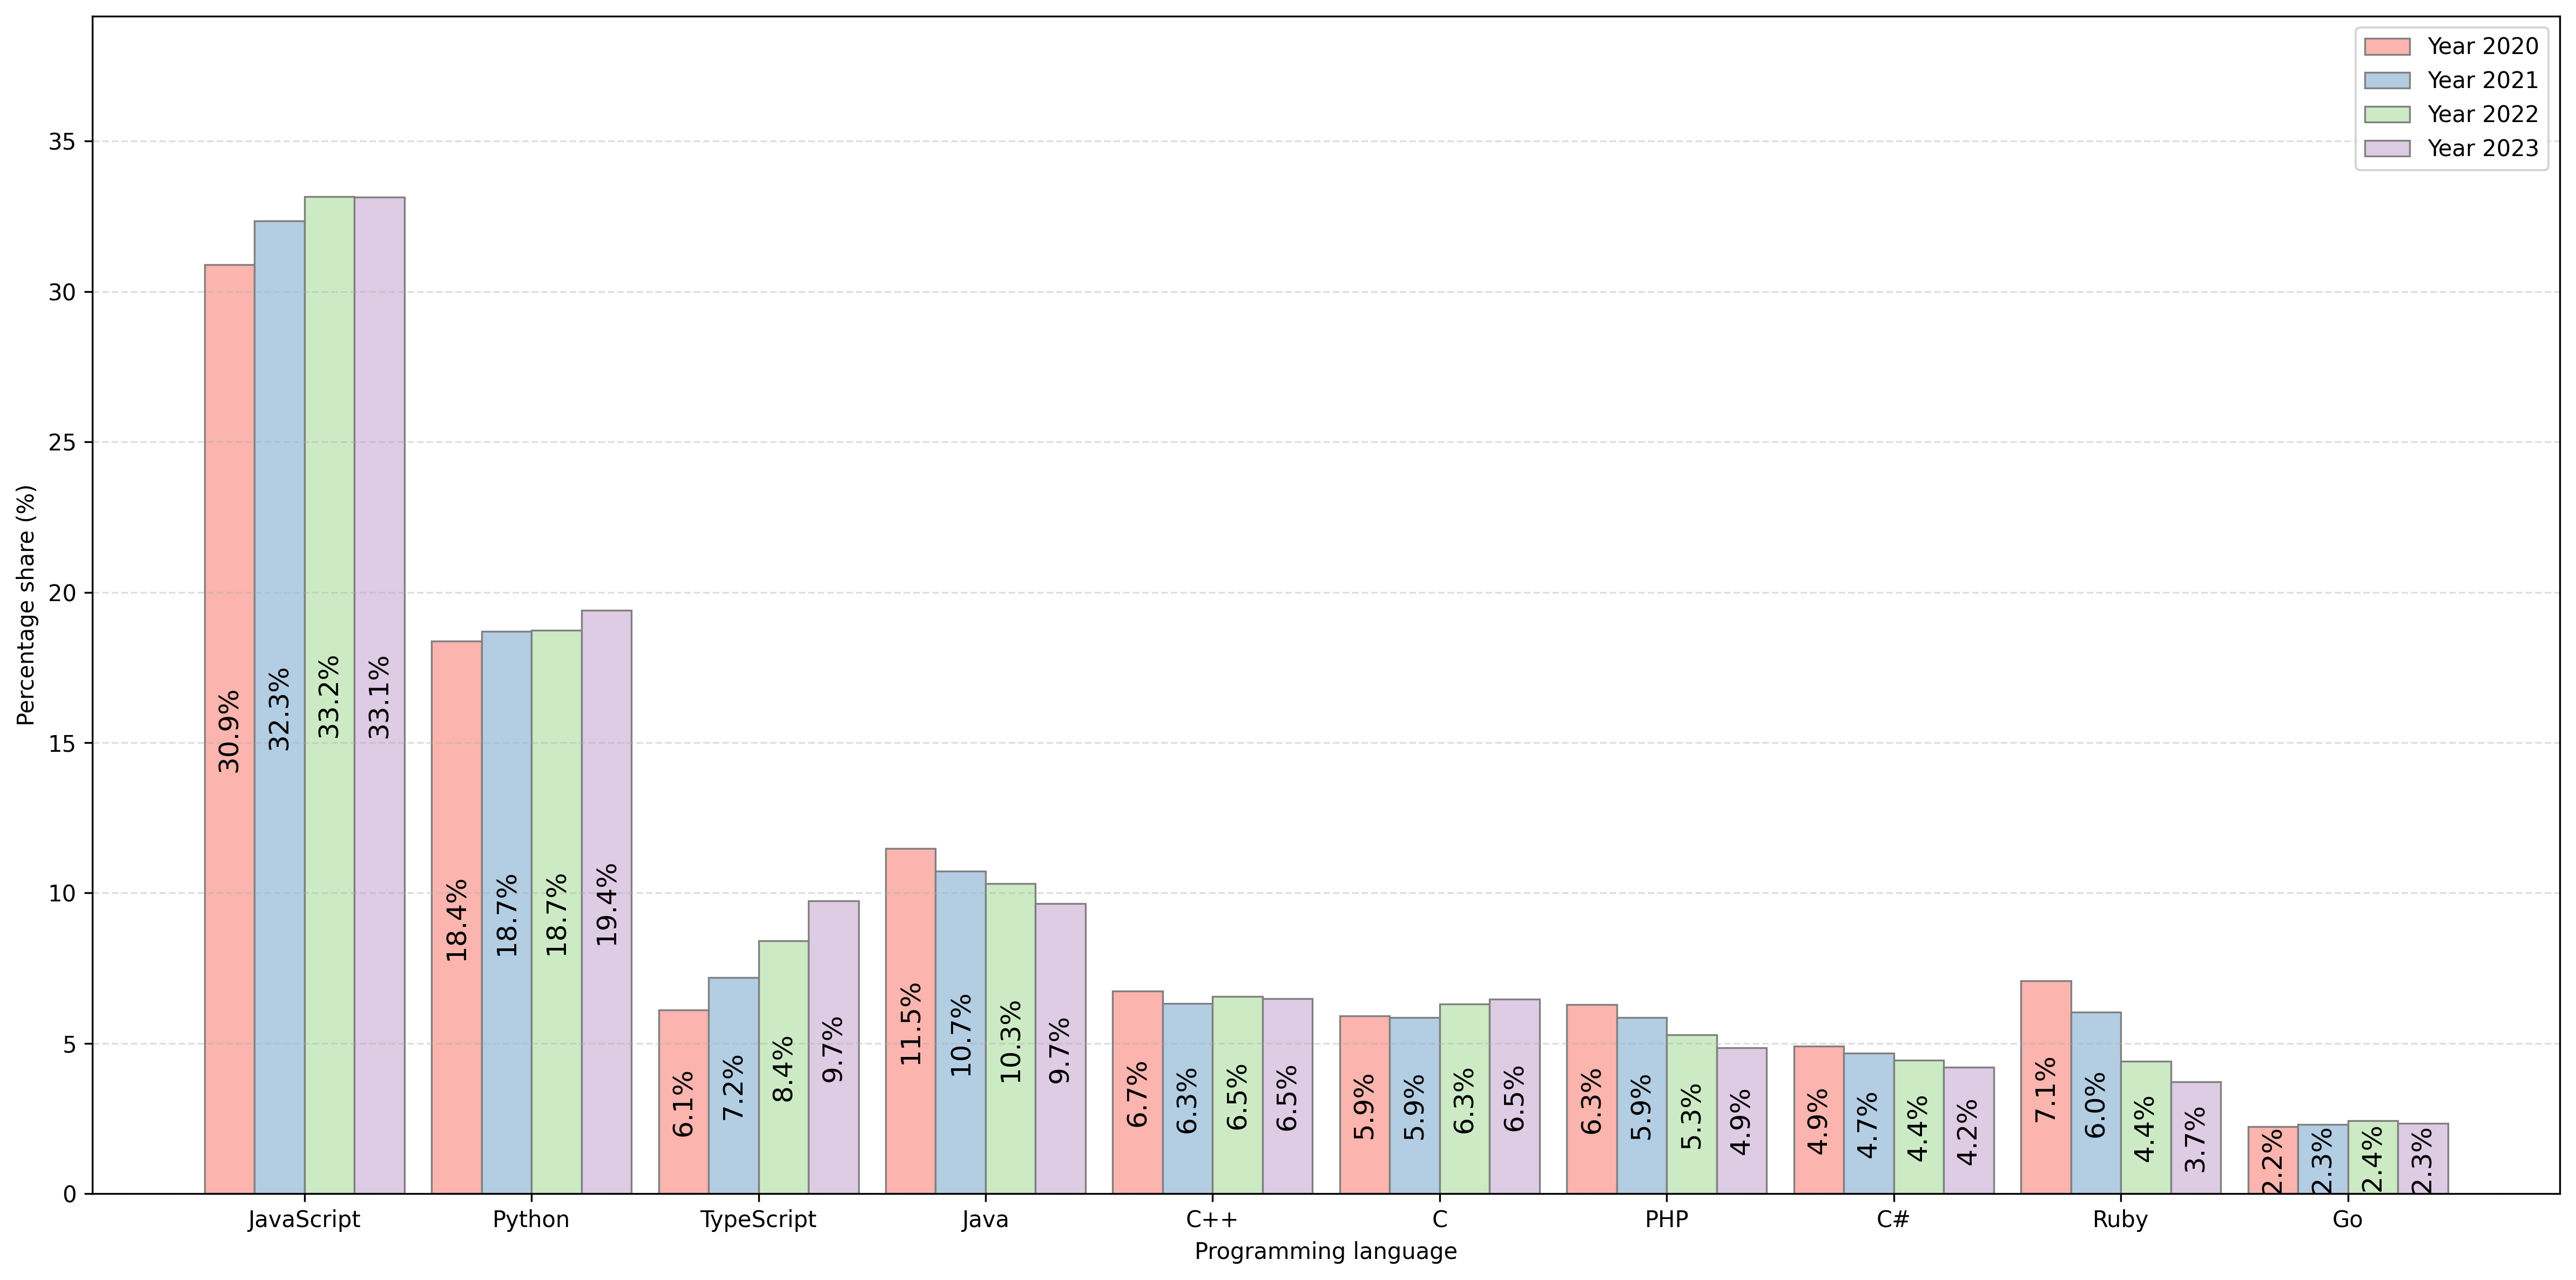
\includegraphics[width=\textwidth]{language_distribution_gpt_available_2020_2023.png}
\caption{Distribución de lenguajes de programación más populares en países con ChatGPT disponible (2020-2023)}
\label{fig:figura1}
\end{figure}

\begin{figure}[htbp]
\centering
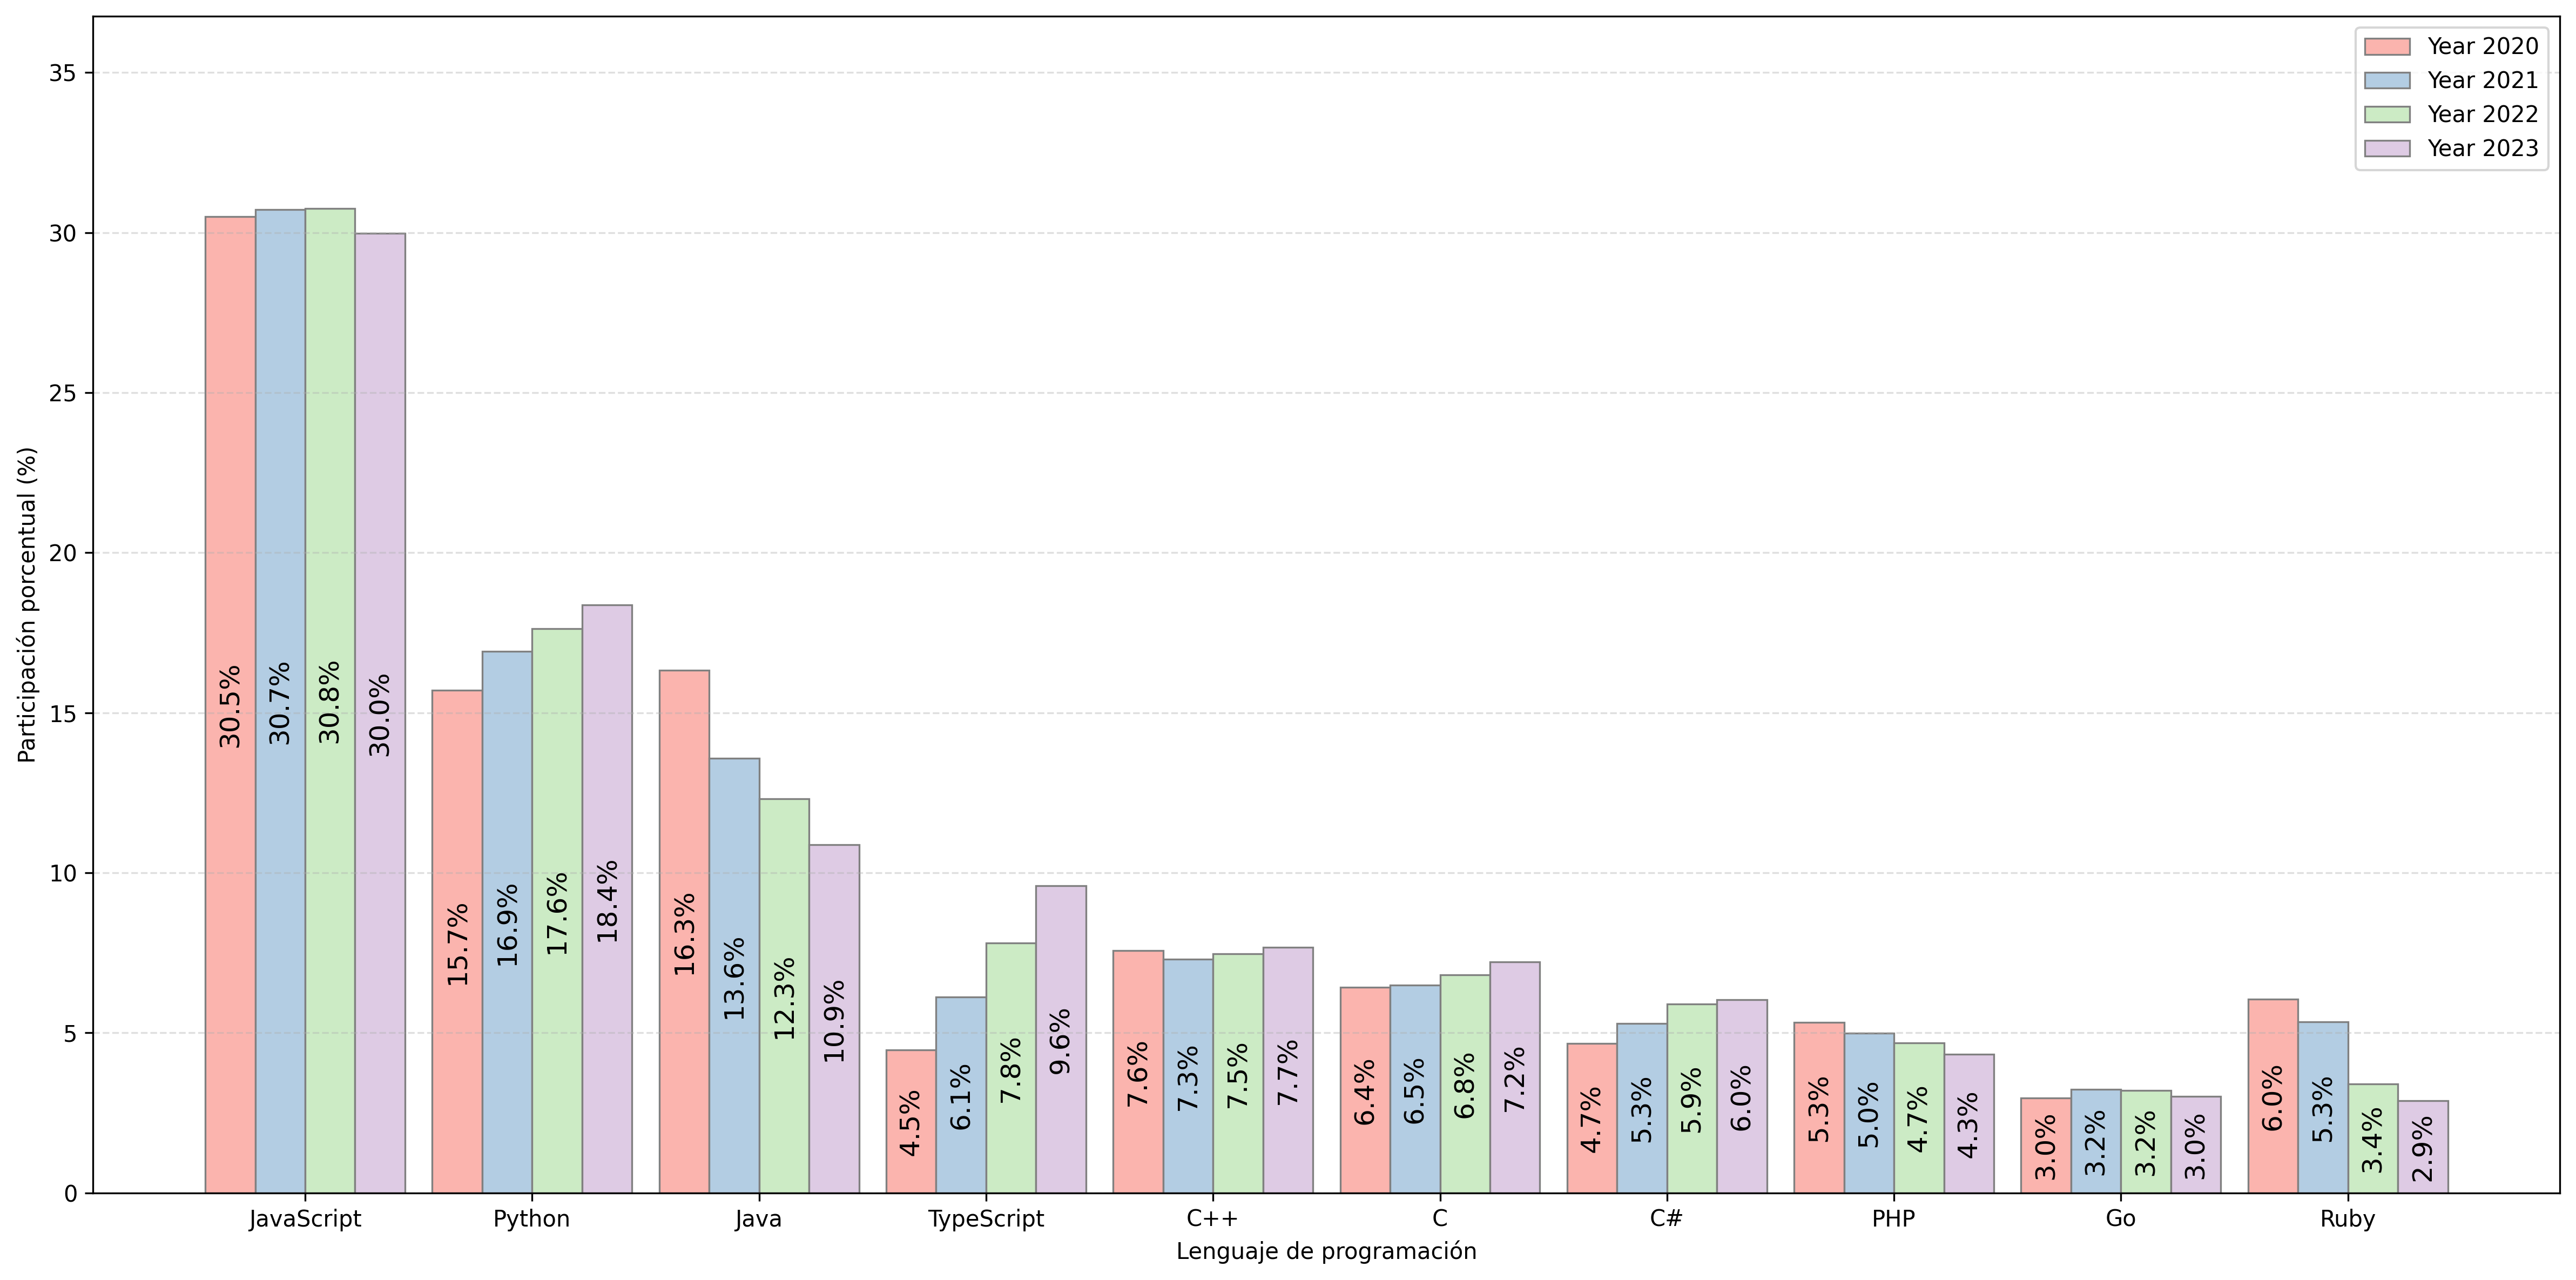
\includegraphics[width=\textwidth]{language_distribution_no_gpt_2020_2023.png}
\caption{Distribución de lenguajes de programación más populares en países sin ChatGPT disponible (2020-2023)}
\label{fig:figura2}
\end{figure}

\begin{figure}[htbp]
\centering
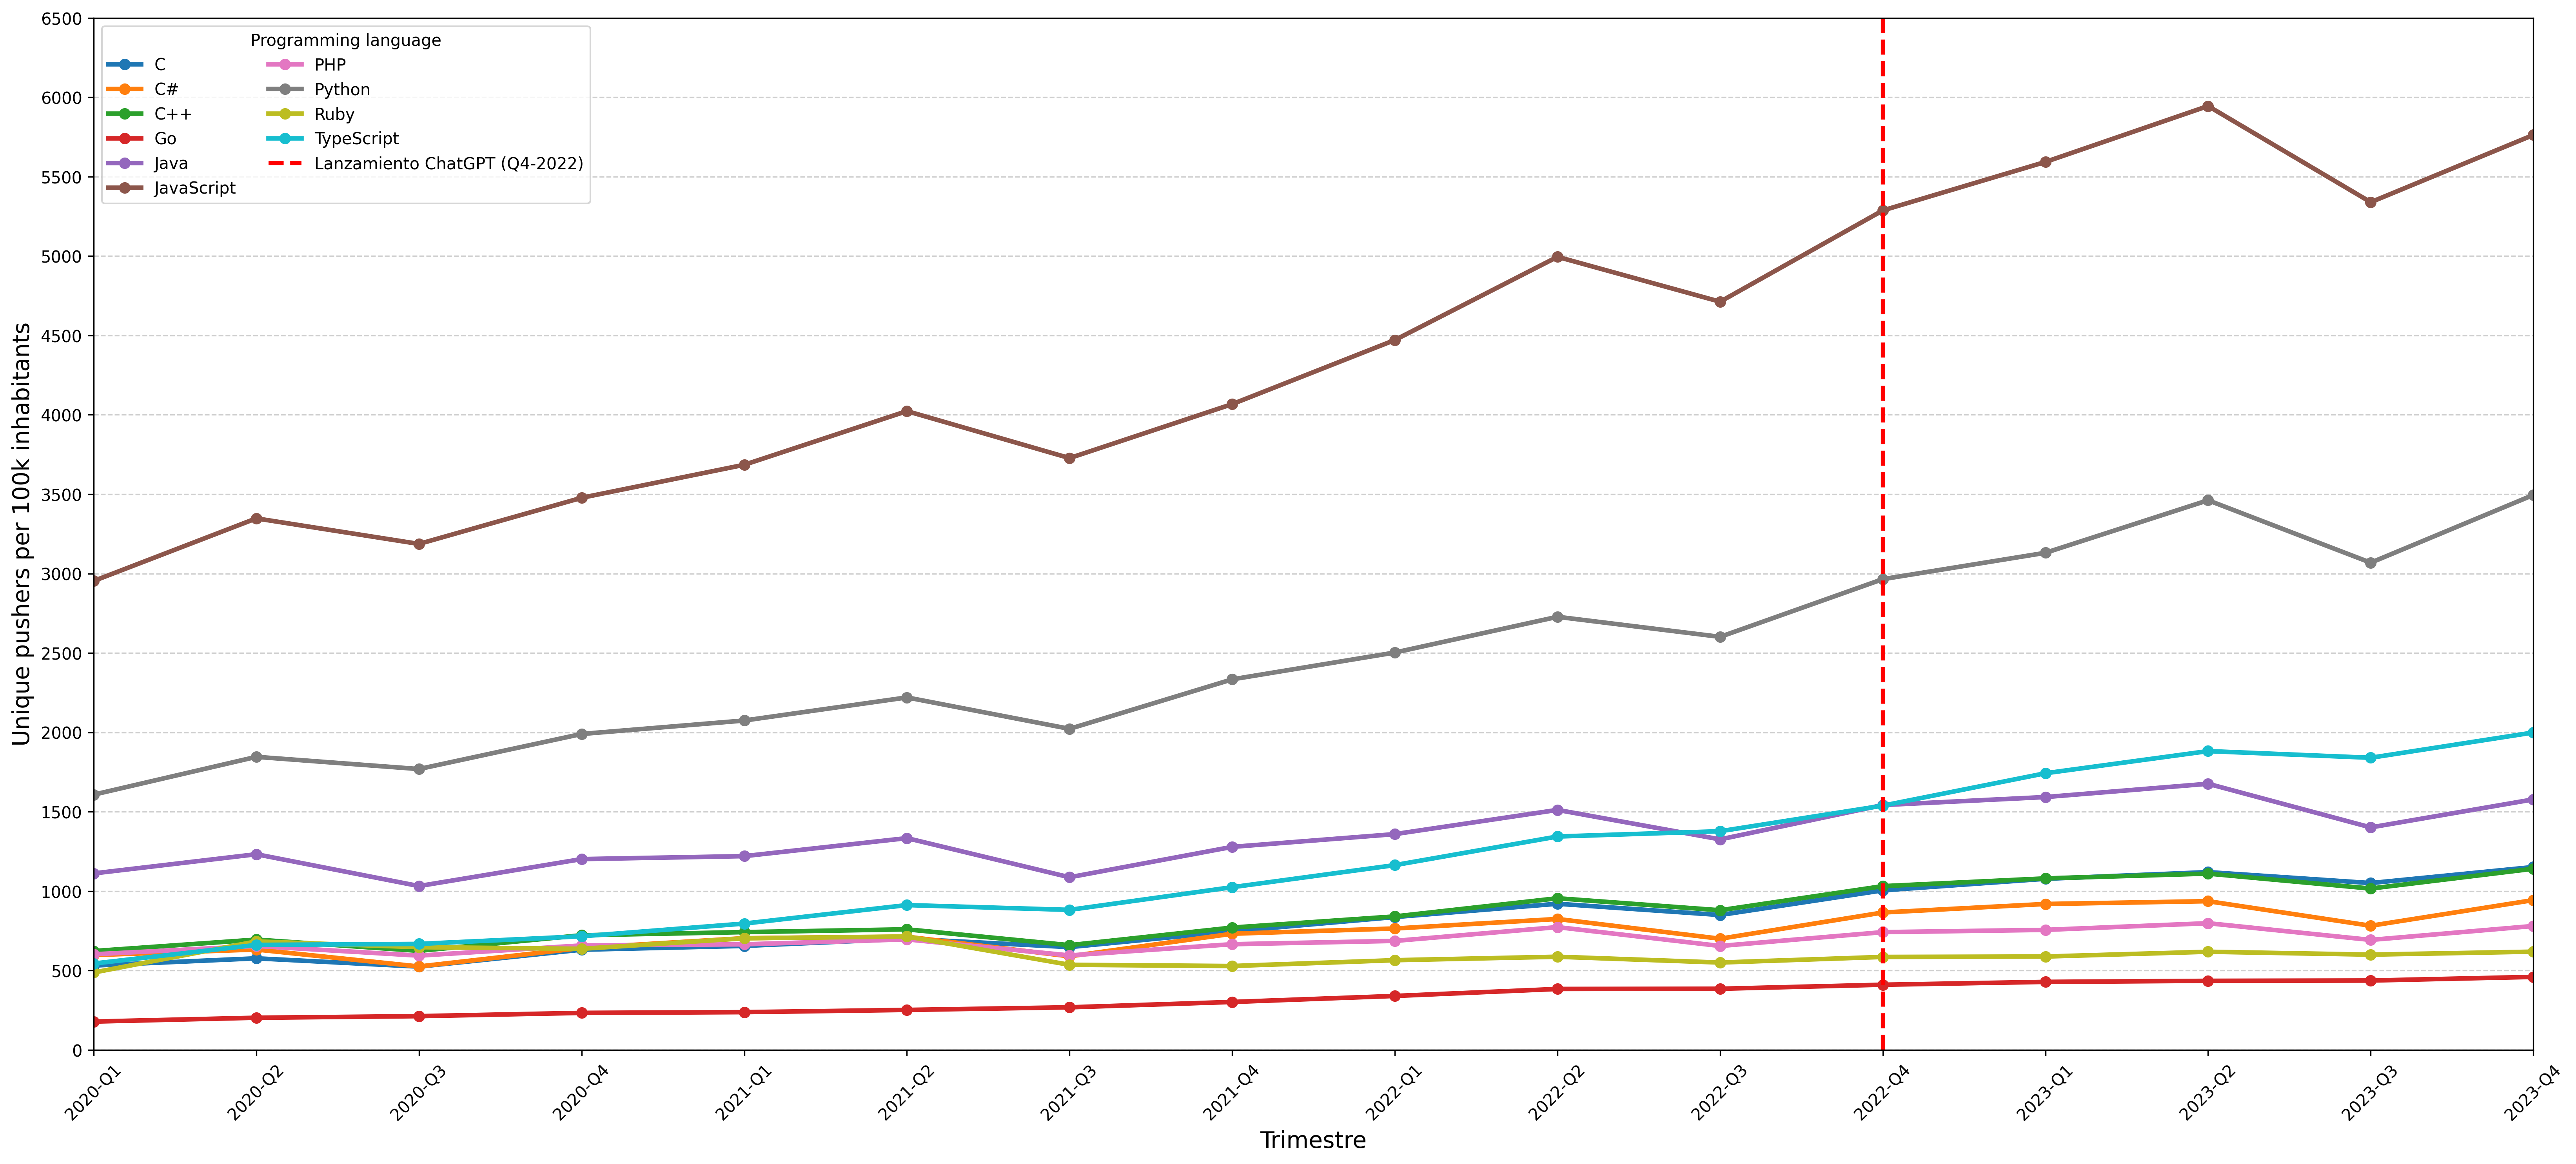
\includegraphics[width=\textwidth]{language_trend_2020_2023.png}
\caption{Tendencia global de \textit{unique pushers} por lenguaje de programación (2020–2023)}
\label{fig:figura3}
\end{figure}

\begin{figure}[htbp]
\centering
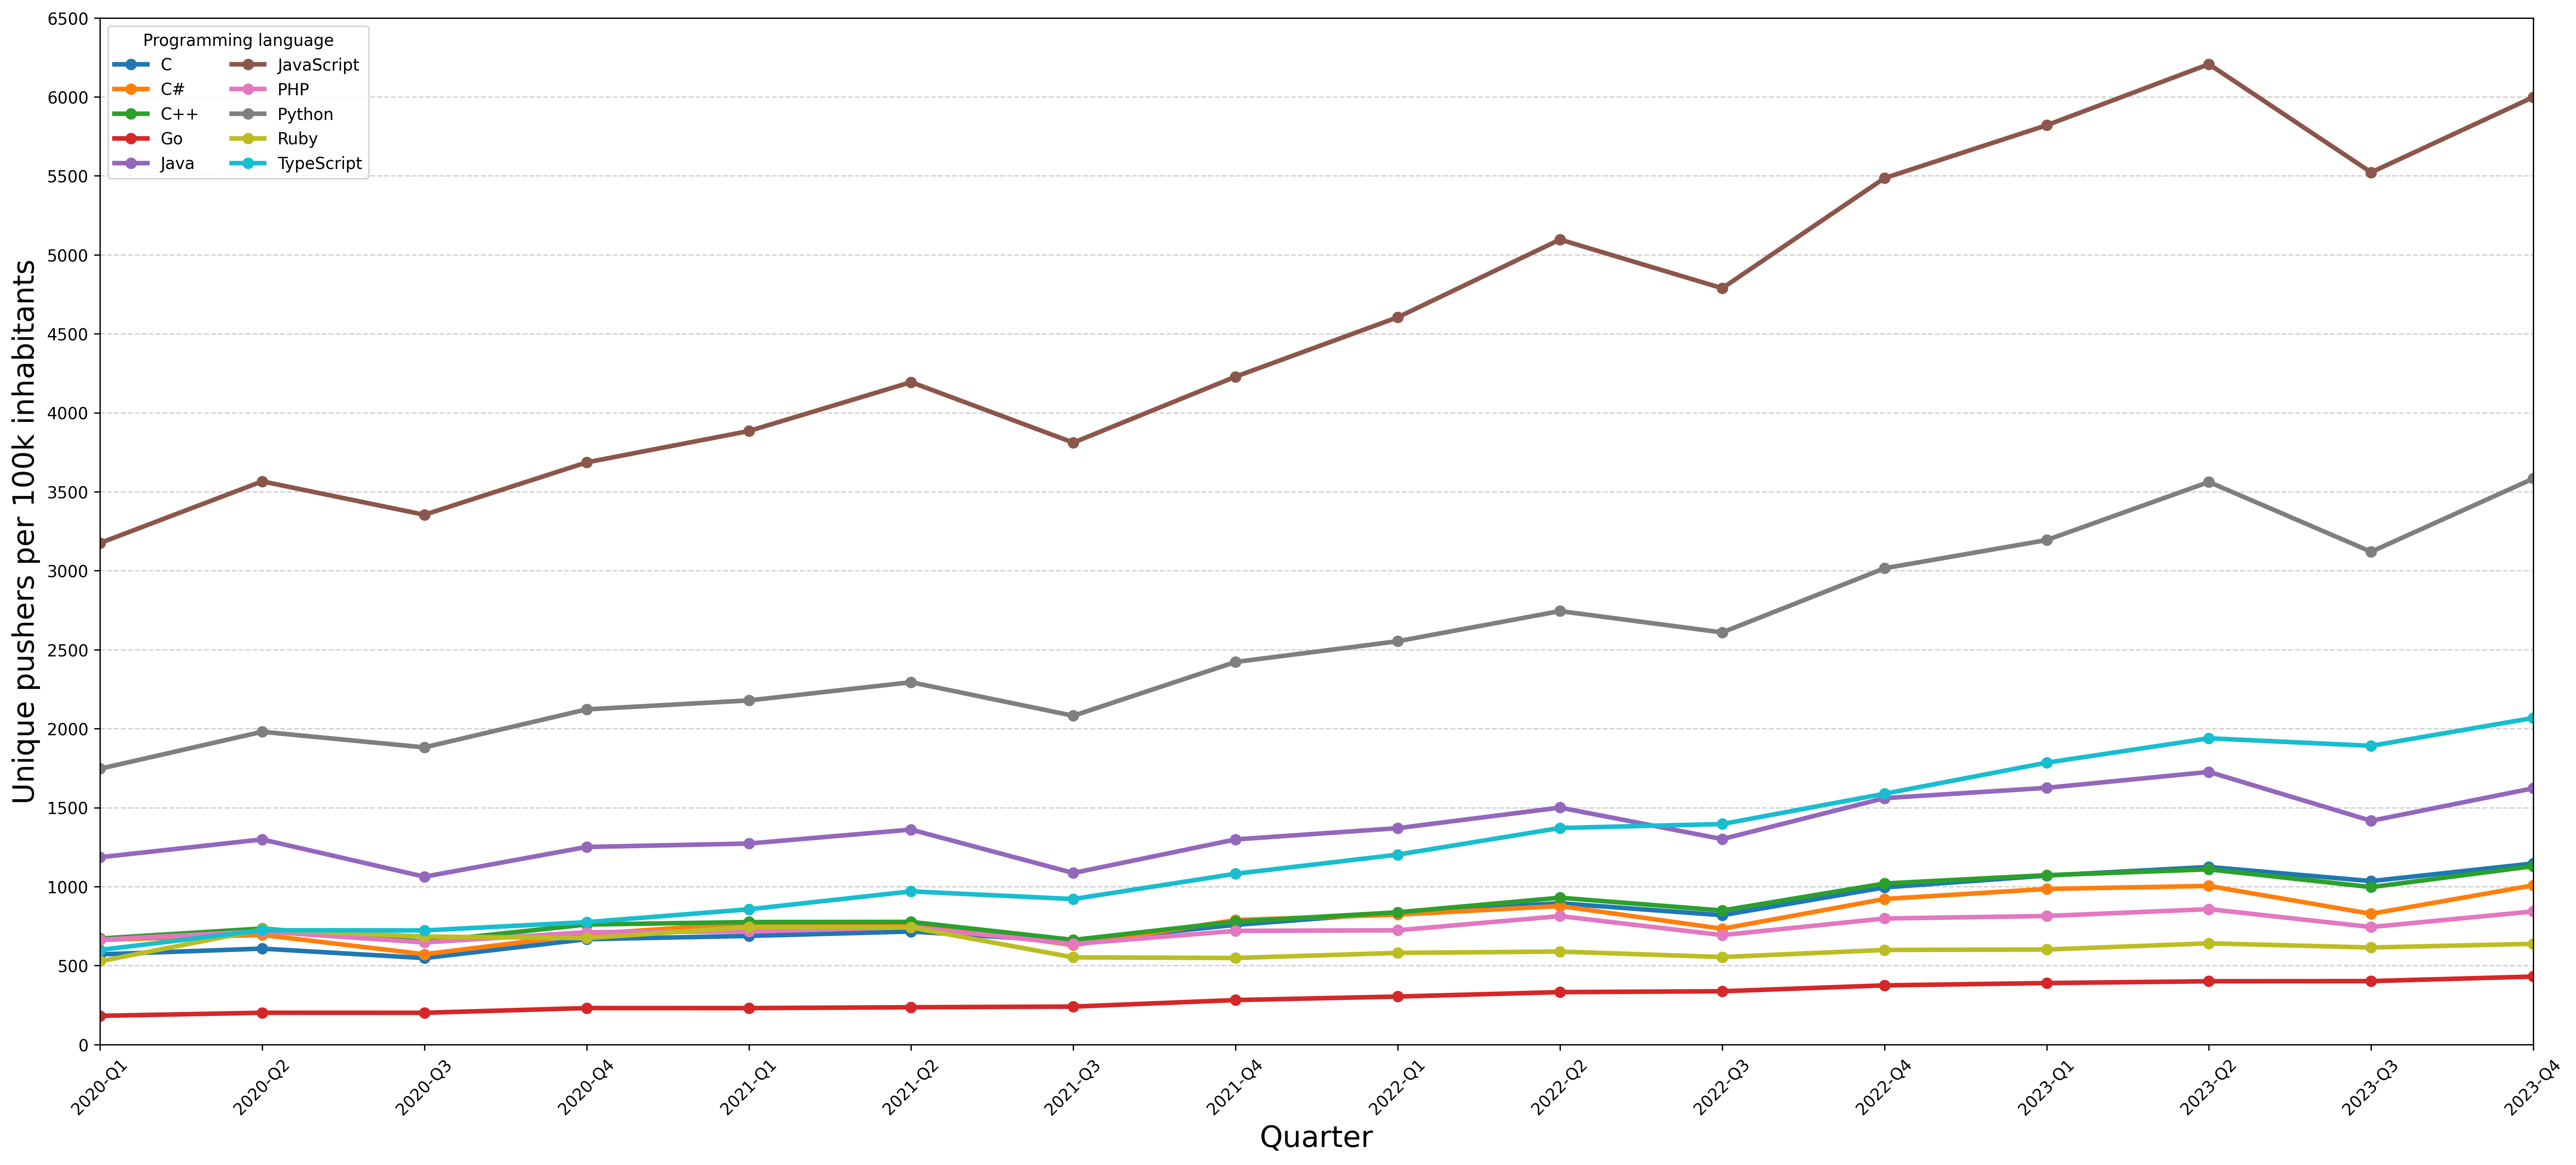
\includegraphics[width=\textwidth]{language_trend_gpt_countries_2020_2023.png}
\caption{Distribución de \textit{unique pushers} según lenguaje en países con ChatGPT (2020–2023)}
\label{fig:figura4}
\end{figure}

\begin{figure}[htbp]
\centering
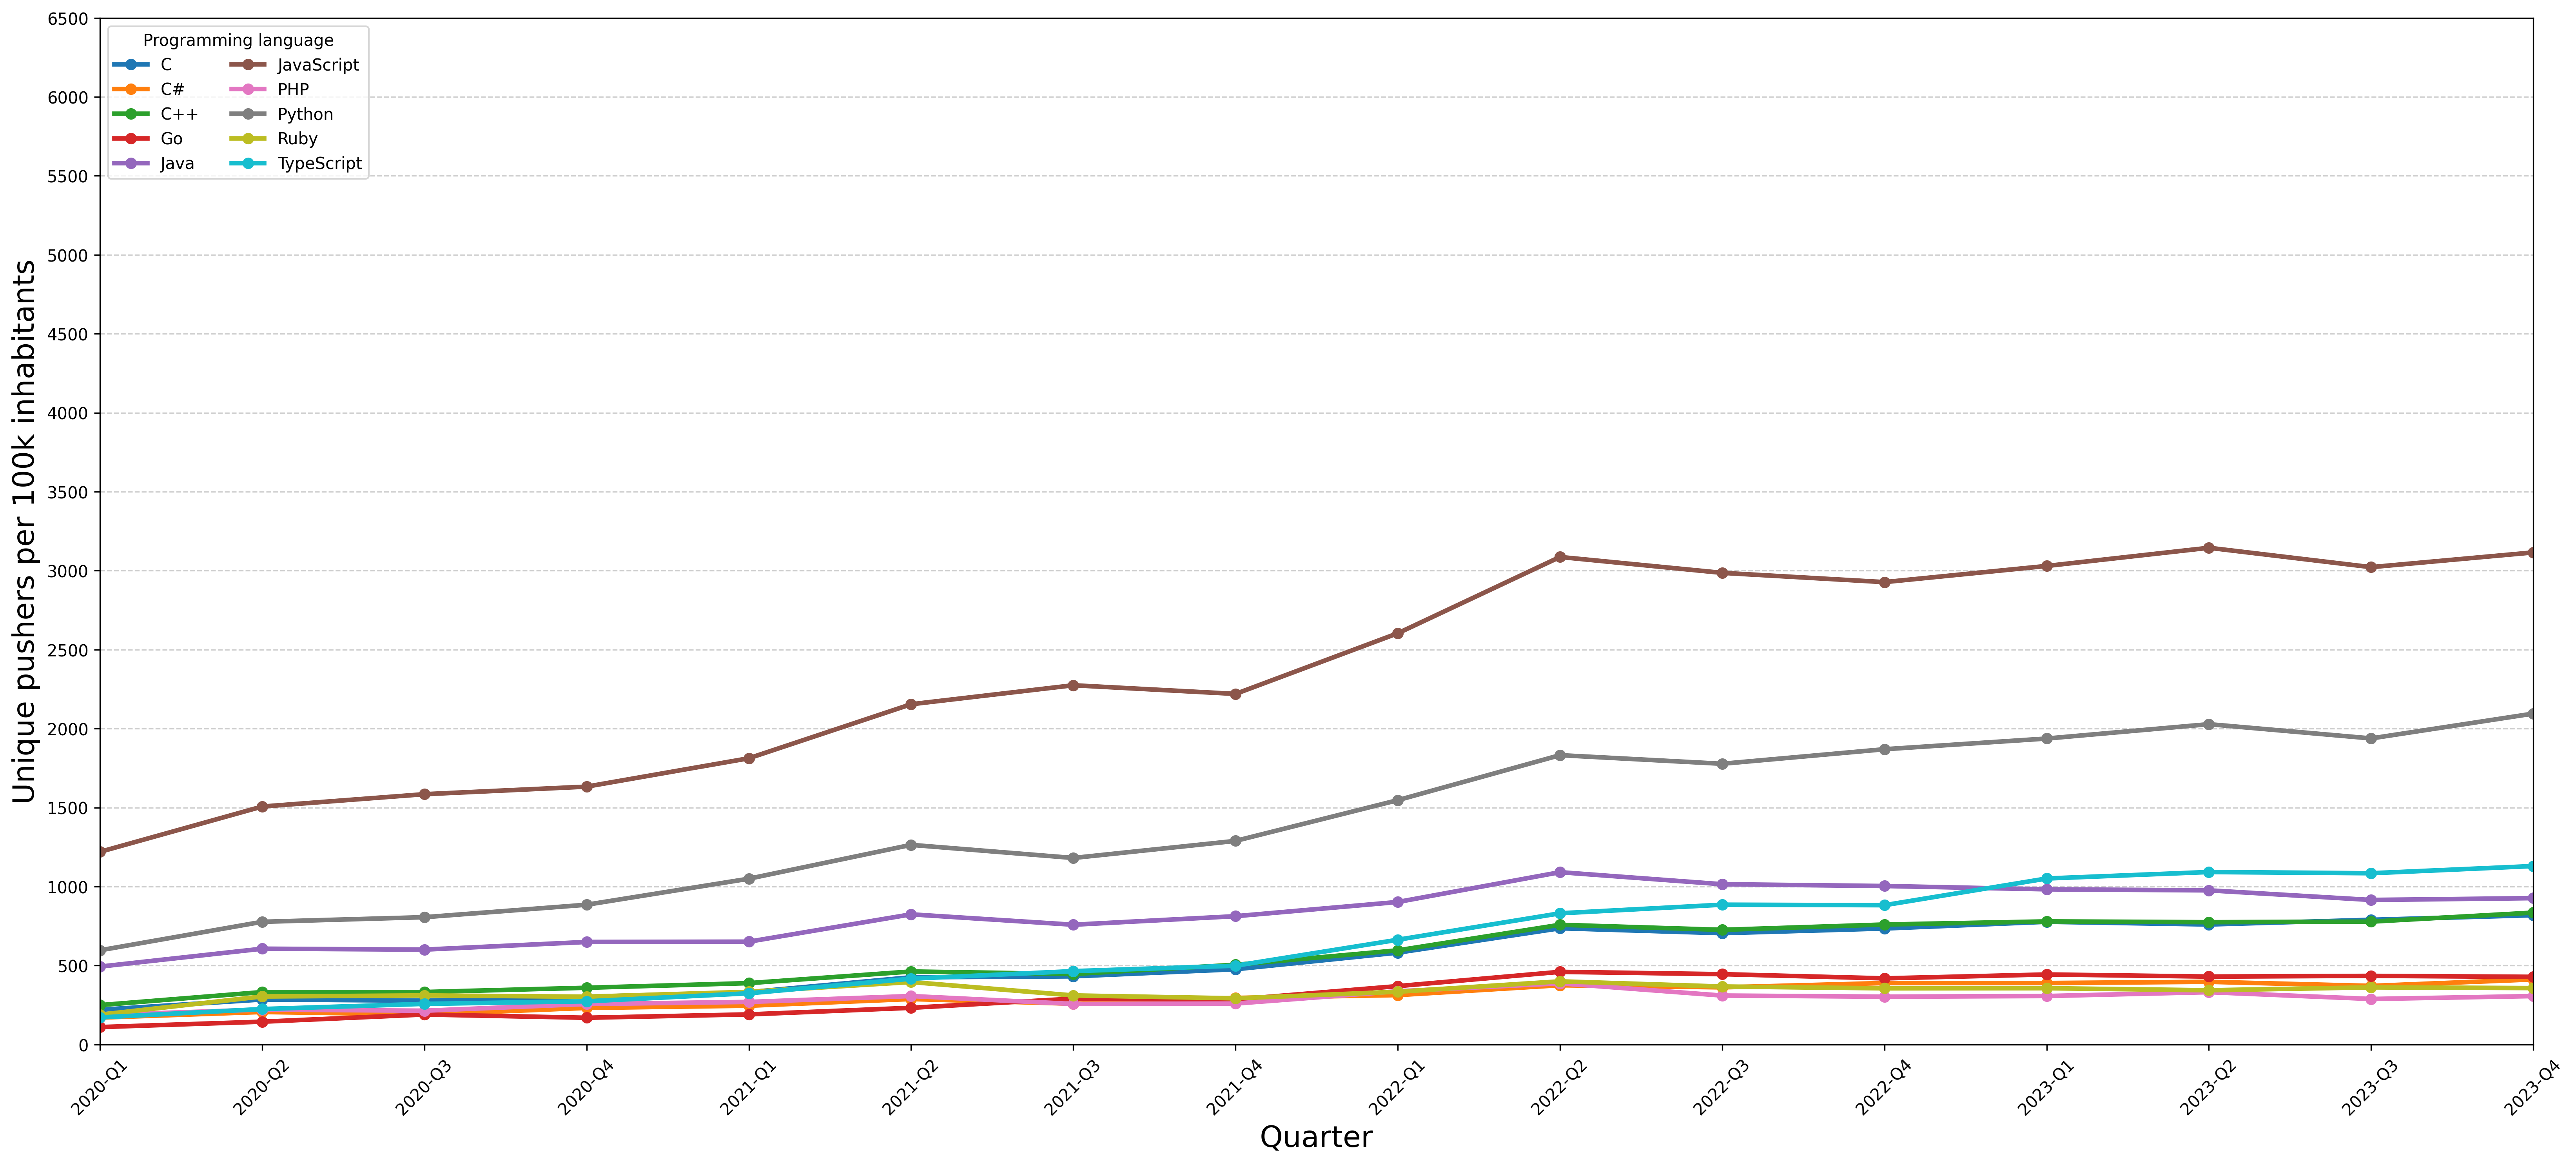
\includegraphics[width=\textwidth]{language_trend_no_gpt_countries_2020_2023.png}
\caption{Distribución de \textit{unique pushers} según lenguaje en países sin ChatGPT (2020–2023)}
\label{fig:figura5}
\end{figure}


% ── Figuras 6–15: tendencias y ponderaciones (DID, SC, SDiD) ─────────────────

\begin{figure}[htbp]
\centering
\begin{subfigure}{\textwidth}\centering
  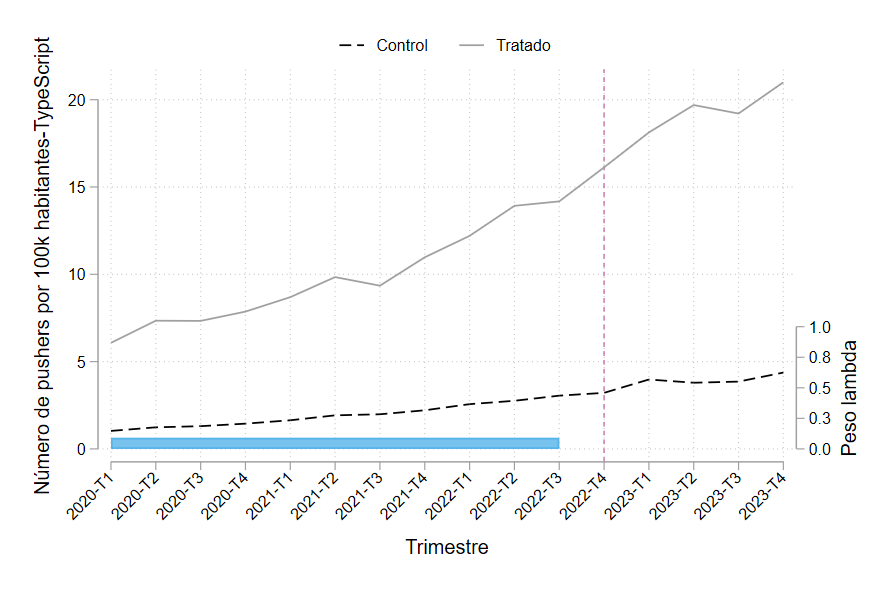
\includegraphics[width=\textwidth]{TypeScriptdid_trends12.png}
  \caption*{(a)–(b) DiD}
\end{subfigure}\\[6pt]
\begin{subfigure}{\textwidth}\centering
  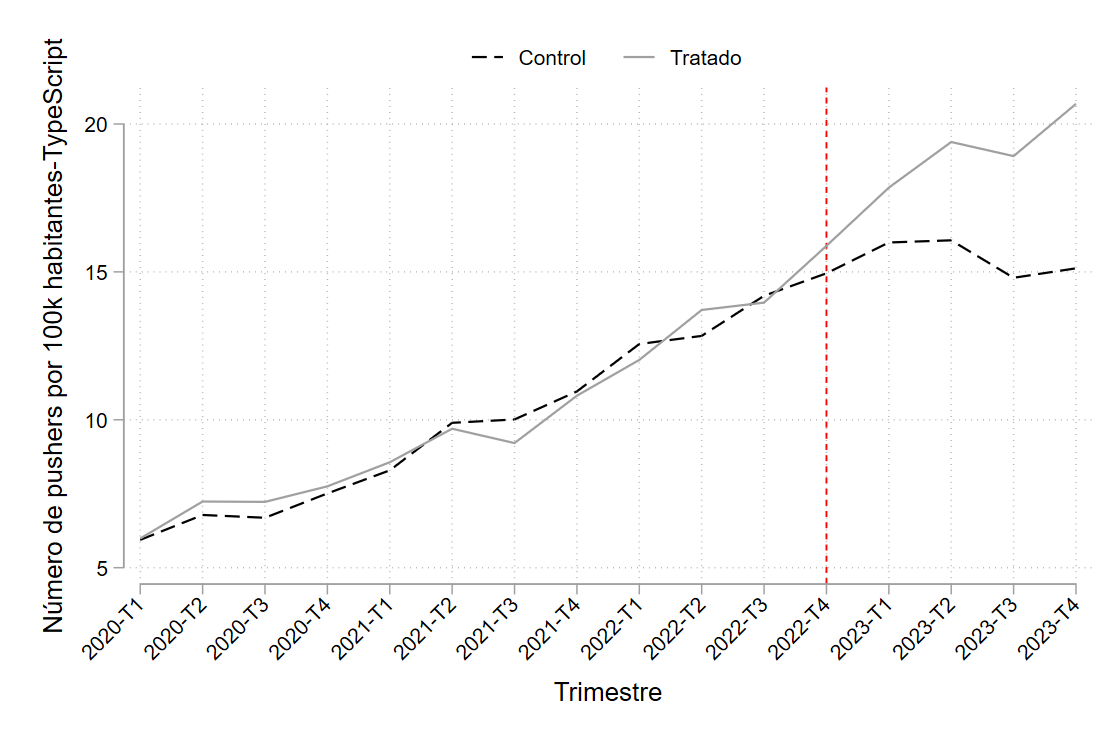
\includegraphics[width=\textwidth]{TypeScriptsc_trends12.png}
  \caption*{(c)–(d) SC}
\end{subfigure}\\[6pt]
\begin{subfigure}{\textwidth}\centering
  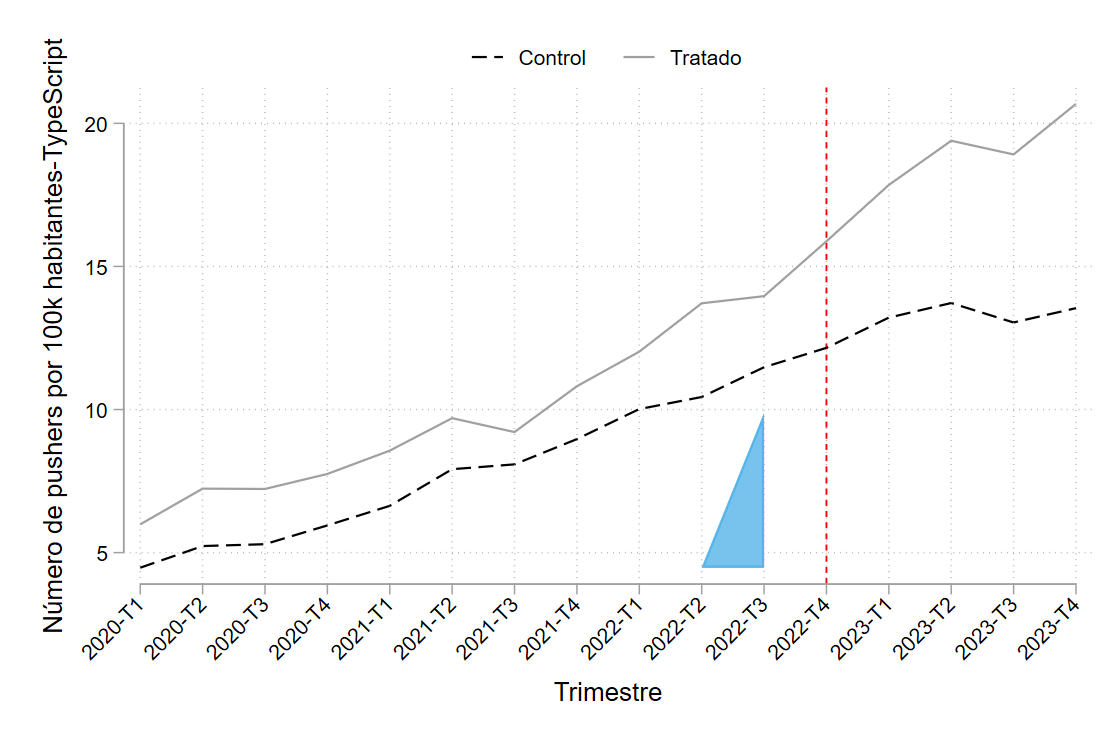
\includegraphics[width=\textwidth]{TypeScriptsdid_trends12.png}
  \caption*{(e)–(f) SDiD}
\end{subfigure}
\caption{Tendencias y ponderaciones estimadas de TypeScript \textit{unique pushers} por cada 100 mil personas}
\label{fig:figura6}
\end{figure}

\begin{figure}[htbp]
\centering
\begin{subfigure}{\textwidth}\centering
  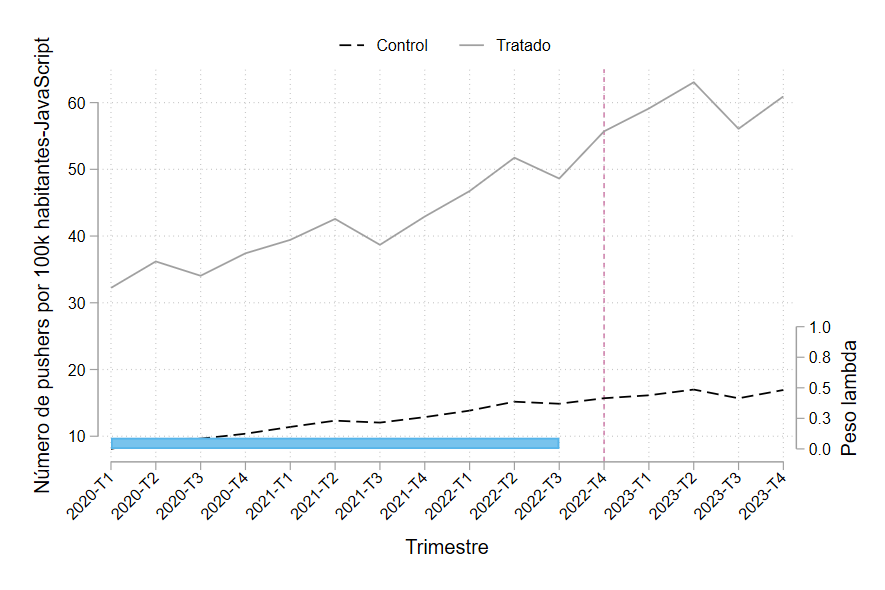
\includegraphics[width=\textwidth]{JavaScriptdid_trends12.png}
  \caption*{(a)–(b) DiD}
\end{subfigure}\\[6pt]
\begin{subfigure}{\textwidth}\centering
  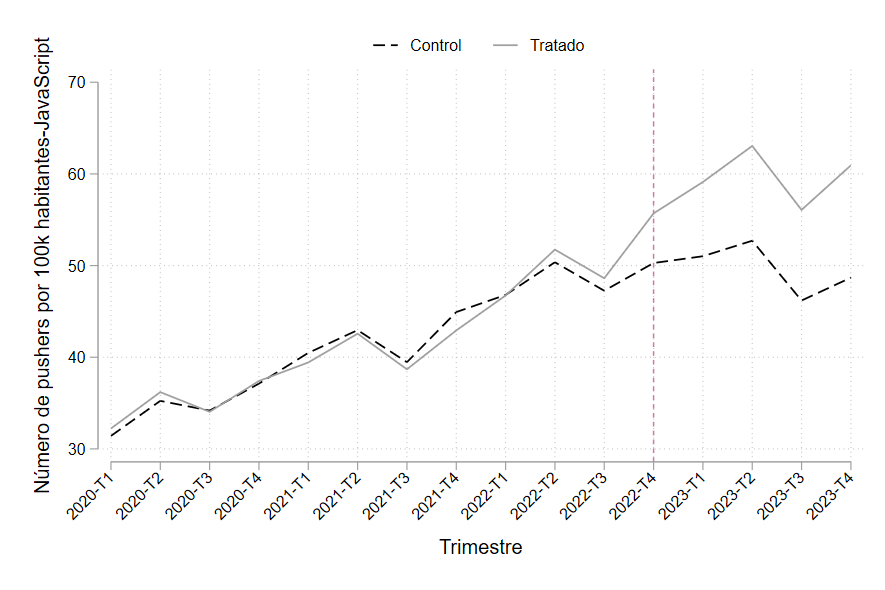
\includegraphics[width=\textwidth]{JavaScriptsc_trends12.png}
  \caption*{(c)–(d) SC}
\end{subfigure}\\[6pt]
\begin{subfigure}{\textwidth}\centering
  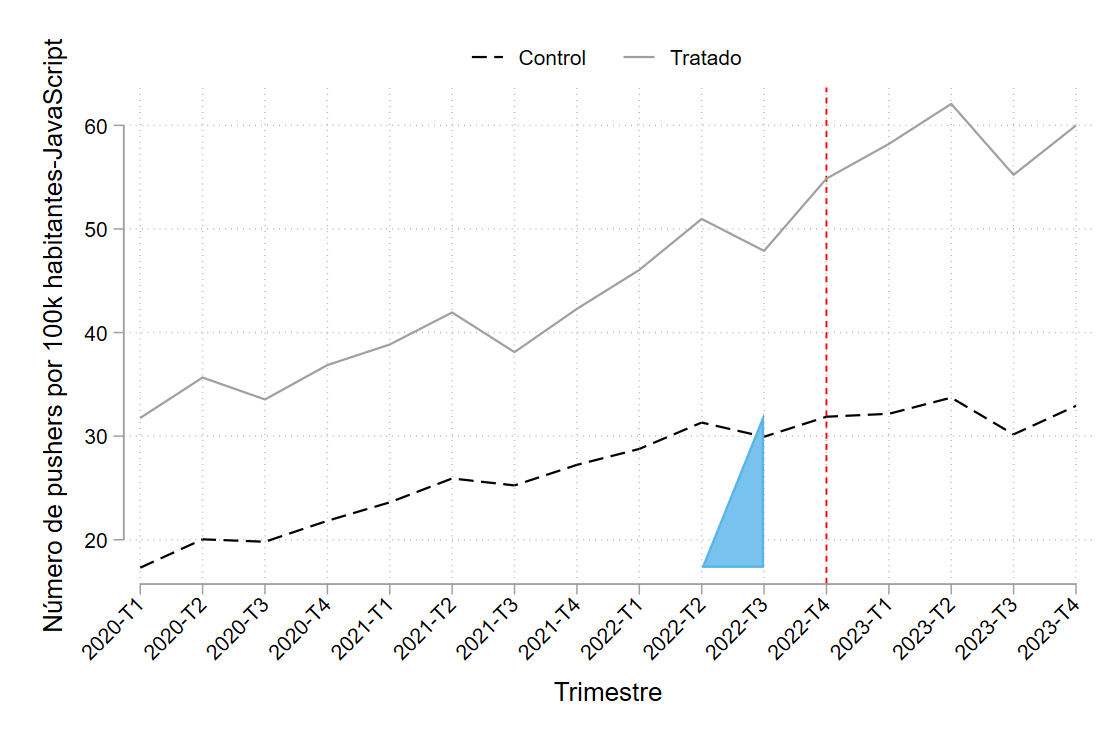
\includegraphics[width=\textwidth]{JavaScriptsdid_trends12.png}
  \caption*{(e)–(f) SDiD}
\end{subfigure}
\caption{Tendencias y ponderaciones estimadas de JavaScript \textit{unique pushers} por cada 100 mil personas}
\label{fig:figura7}
\end{figure}

\begin{figure}[htbp]
\centering
\begin{subfigure}{\textwidth}\centering
  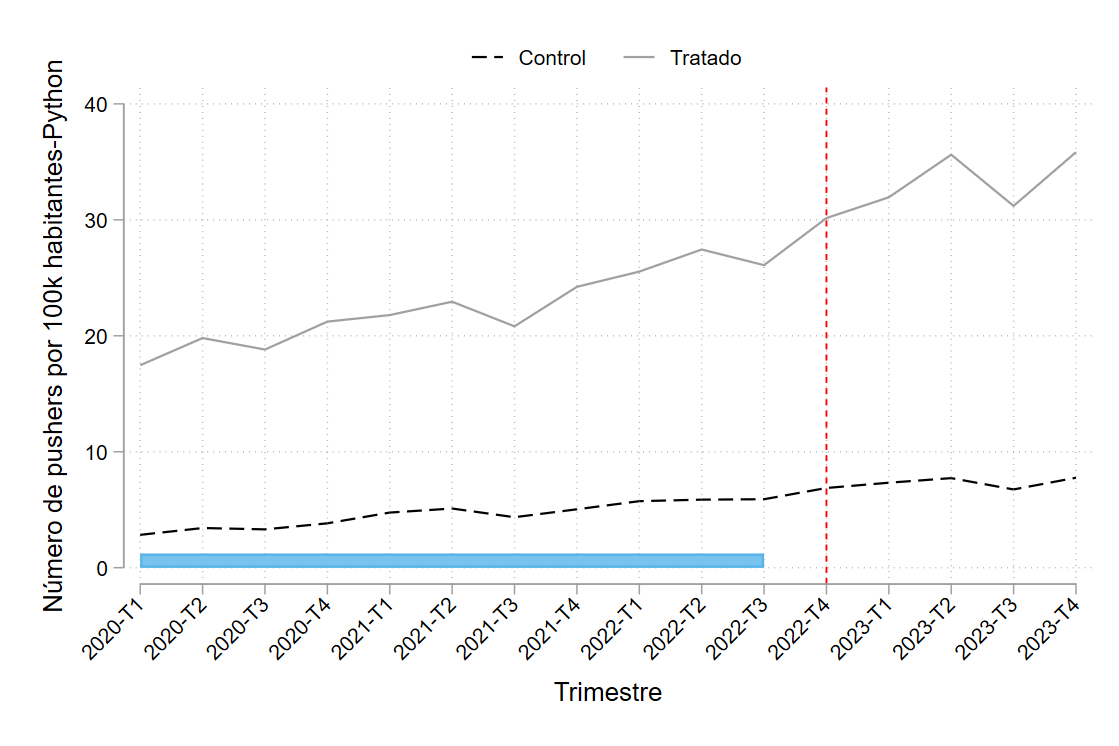
\includegraphics[width=\textwidth]{Pythondid_trends12.png}
  \caption*{(a)–(b) DiD}
\end{subfigure}\\[6pt]
\begin{subfigure}{\textwidth}\centering
  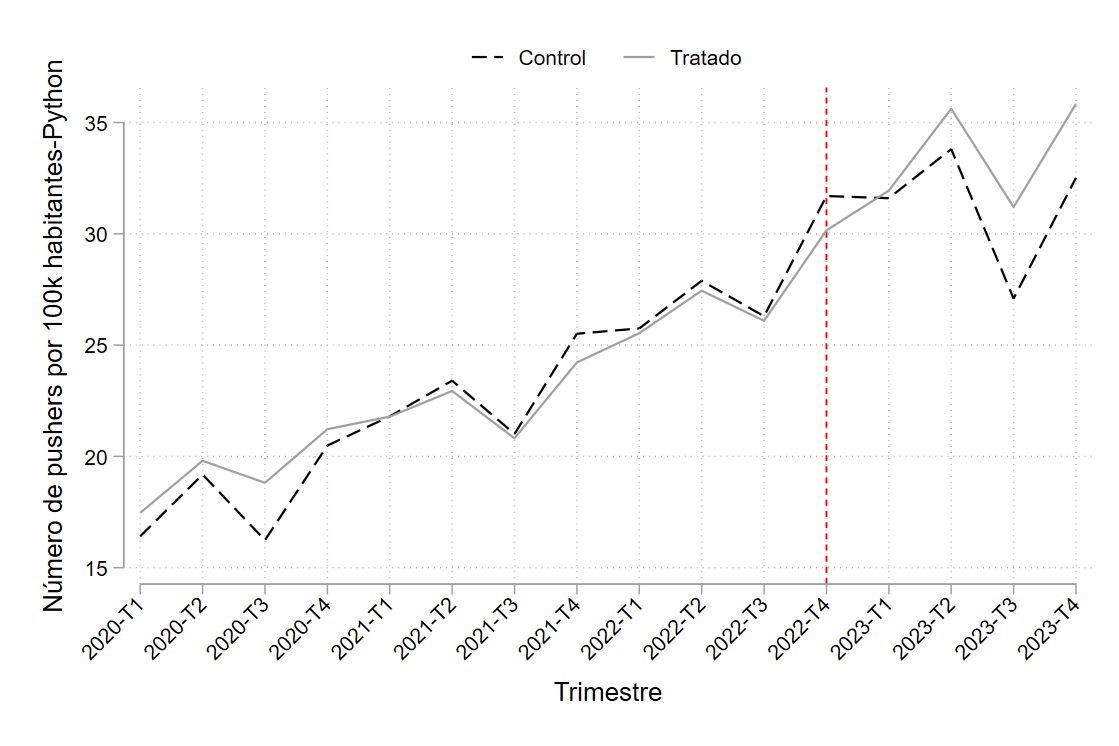
\includegraphics[width=\textwidth]{Pythonsc_trends12.png}
  \caption*{(c)–(d) SC}
\end{subfigure}\\[6pt]
\begin{subfigure}{\textwidth}\centering
  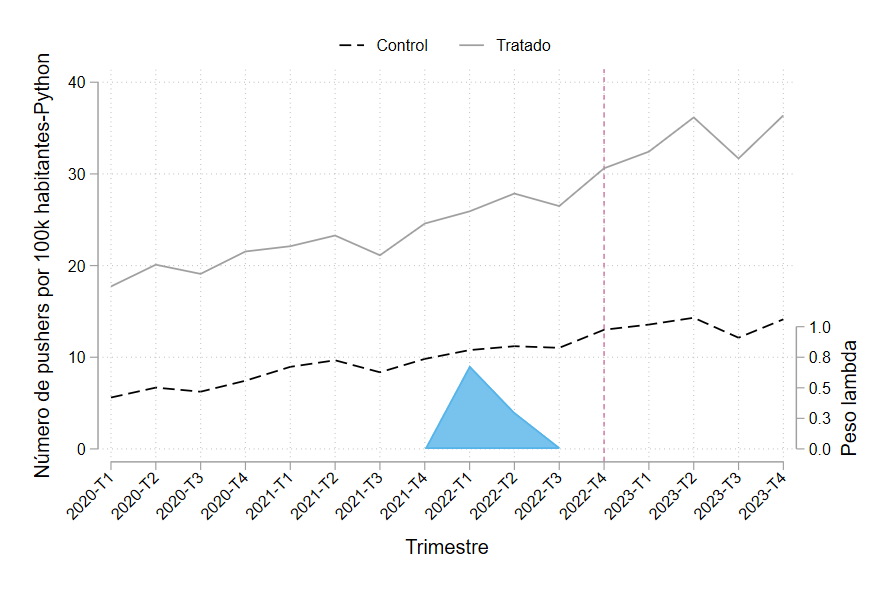
\includegraphics[width=\textwidth]{Pythonsdid_trends12.png}
  \caption*{(e)–(f) SDiD}
\end{subfigure}
\caption{Tendencias y ponderaciones estimadas de Python \textit{unique pushers} por cada 100 mil personas}
\label{fig:figura8}
\end{figure}

\begin{figure}[htbp]
\centering
\begin{subfigure}{\textwidth}\centering
  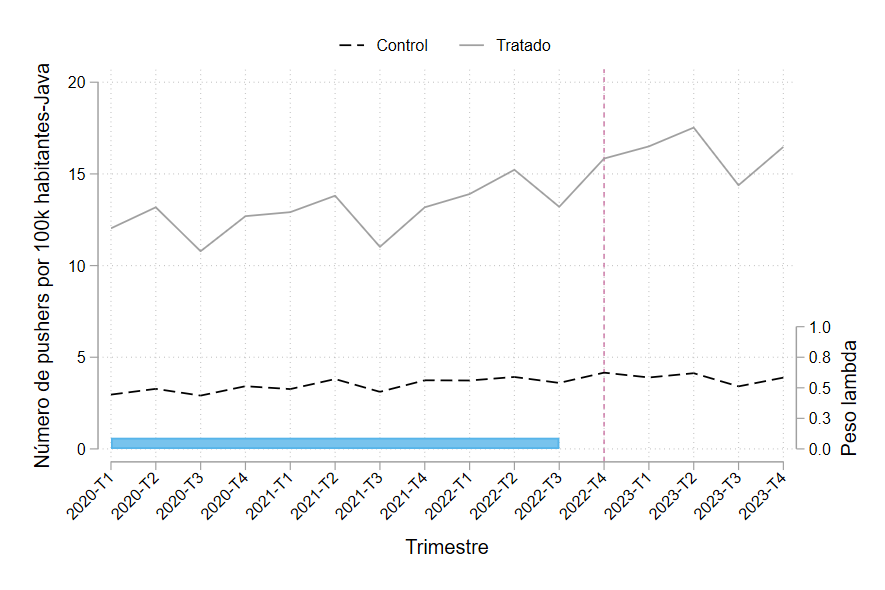
\includegraphics[width=\textwidth]{Javadid_trends12.png}
  \caption*{(a)–(b) DiD}
\end{subfigure}\\[6pt]
\begin{subfigure}{\textwidth}\centering
  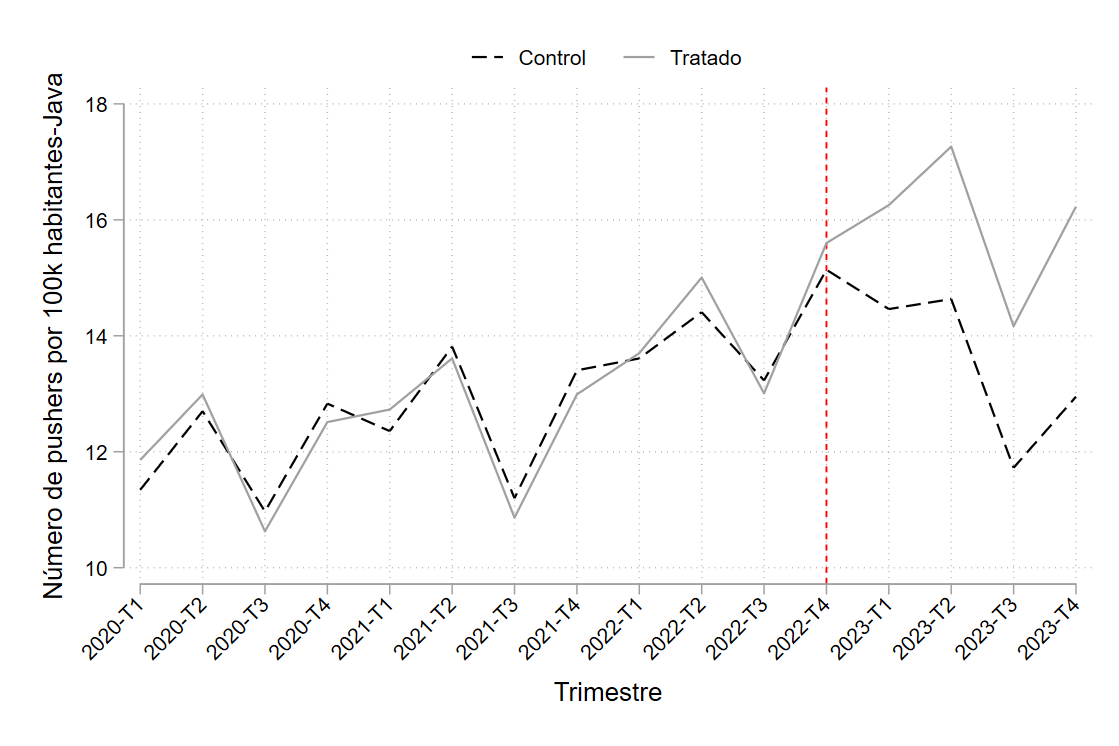
\includegraphics[width=\textwidth]{Javasc_trends12.png}
  \caption*{(c)–(d) SC}
\end{subfigure}\\[6pt]
\begin{subfigure}{\textwidth}\centering
  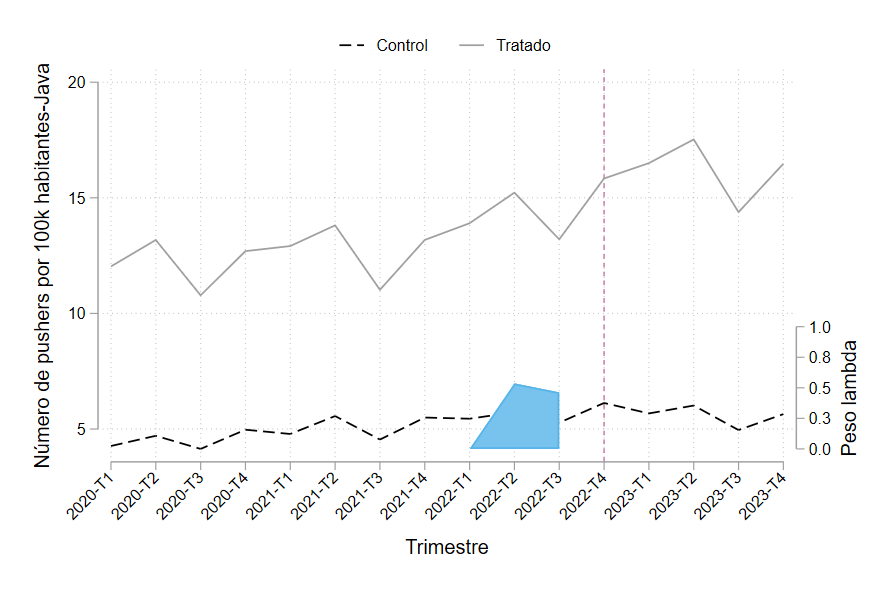
\includegraphics[width=\textwidth]{Javasdid_trends12.png}
  \caption*{(e)–(f) SDiD}
\end{subfigure}
\caption{Tendencias y ponderaciones estimadas de Java \textit{unique pushers} por cada 100 mil personas}
\label{fig:figura9}
\end{figure}

\begin{figure}[htbp]
\centering
\begin{subfigure}{\textwidth}\centering
  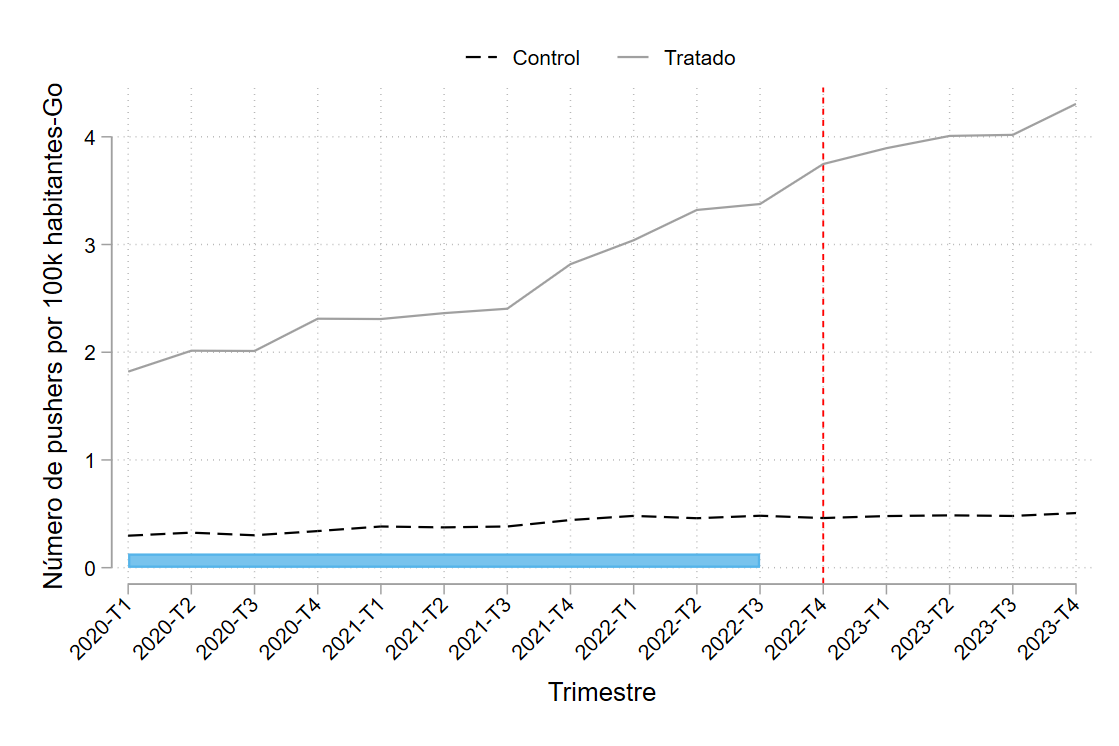
\includegraphics[width=\textwidth]{Godid_trends12.png}
  \caption*{(a)–(b) DiD}
\end{subfigure}\\[6pt]
\begin{subfigure}{\textwidth}\centering
  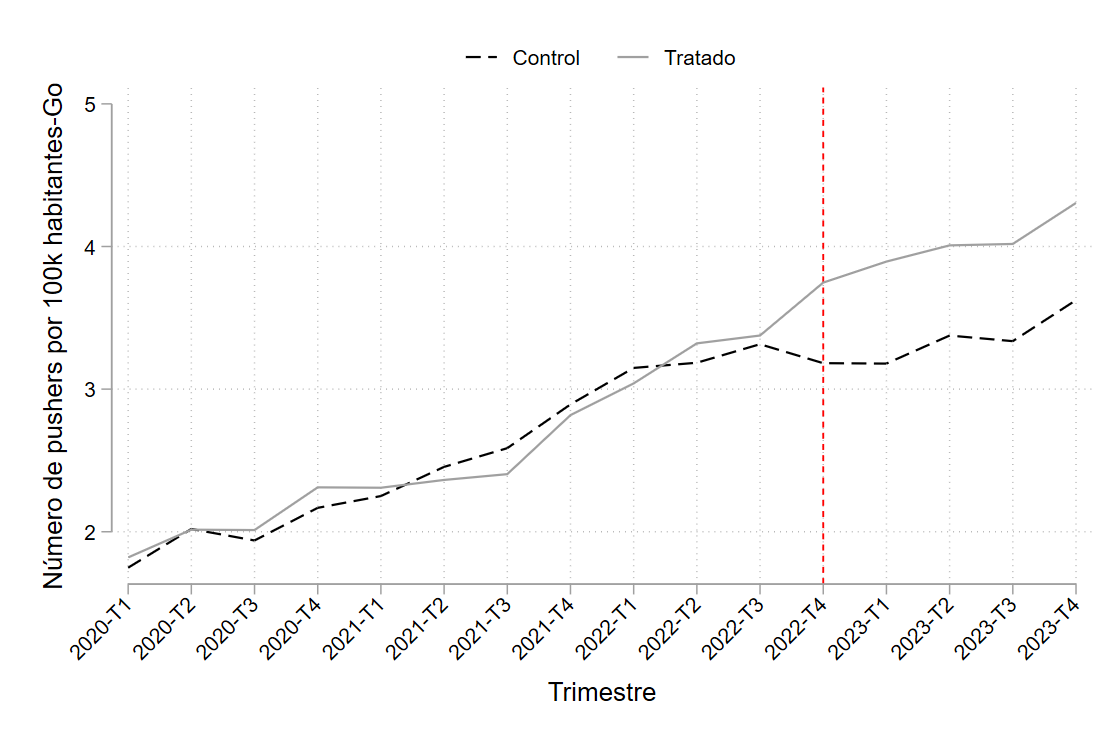
\includegraphics[width=\textwidth]{Gosc_trends12.png}
  \caption*{(c)–(d) SC}
\end{subfigure}\\[6pt]
\begin{subfigure}{\textwidth}\centering
  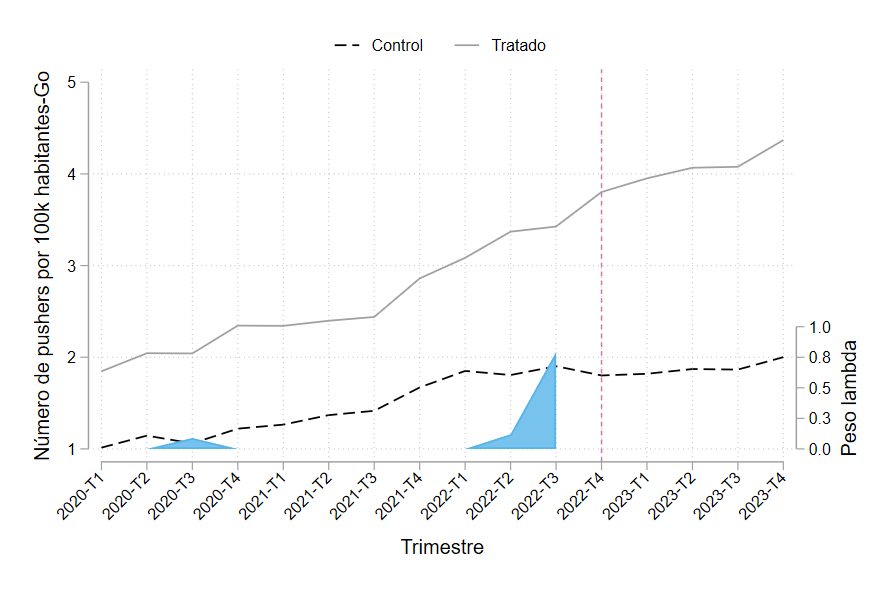
\includegraphics[width=\textwidth]{Gosdid_trends12.png}
  \caption*{(e)–(f) SDiD}
\end{subfigure}
\caption{Tendencias y ponderaciones estimadas de Go \textit{unique pushers} por cada 100 mil personas}
\label{fig:figura10}
\end{figure}

\begin{figure}[htbp]
\centering
\begin{subfigure}{\textwidth}\centering
  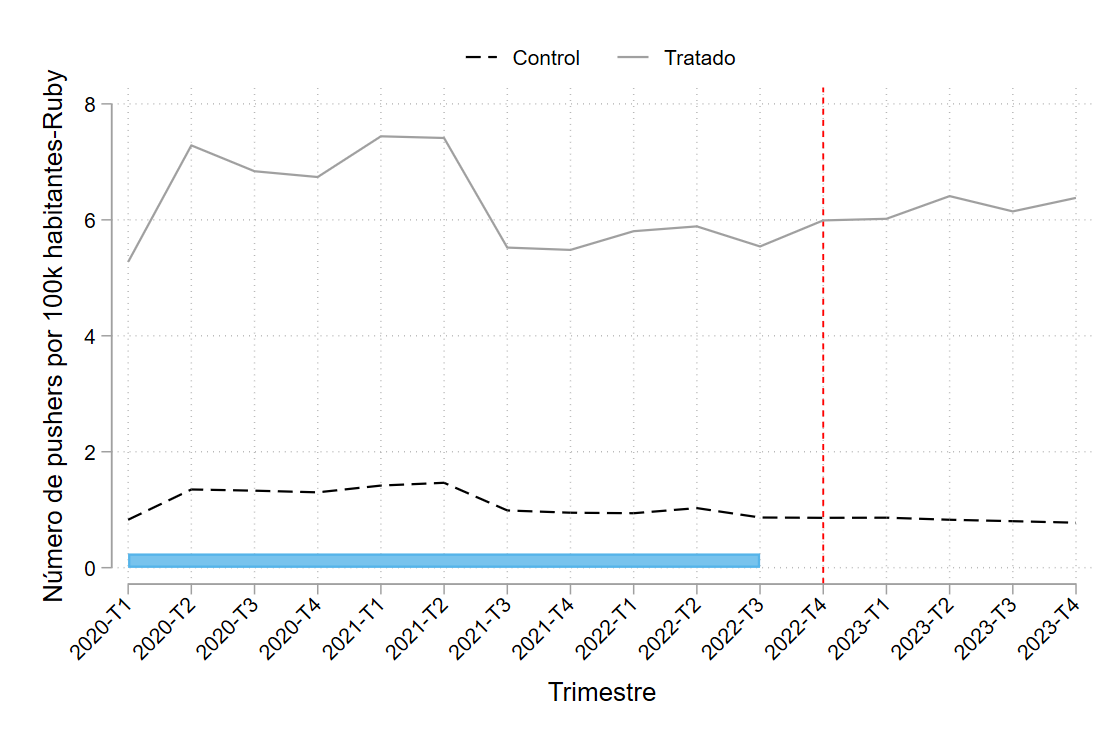
\includegraphics[width=\textwidth]{Rubydid_trends12.png}
  \caption*{(a)–(b) DiD}
\end{subfigure}\\[6pt]
\begin{subfigure}{\textwidth}\centering
  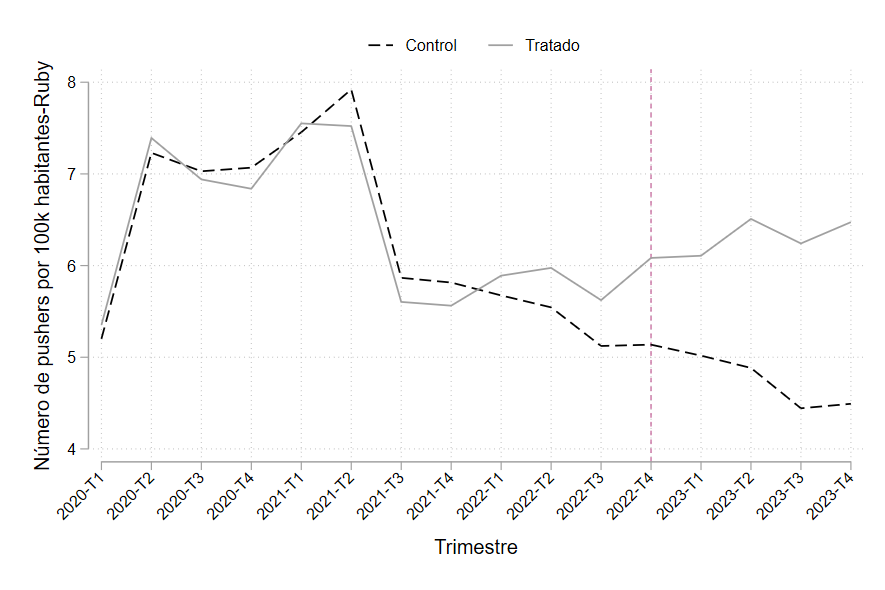
\includegraphics[width=\textwidth]{Rubysc_trends12.png}
  \caption*{(c)–(d) SC}
\end{subfigure}\\[6pt]
\begin{subfigure}{\textwidth}\centering
  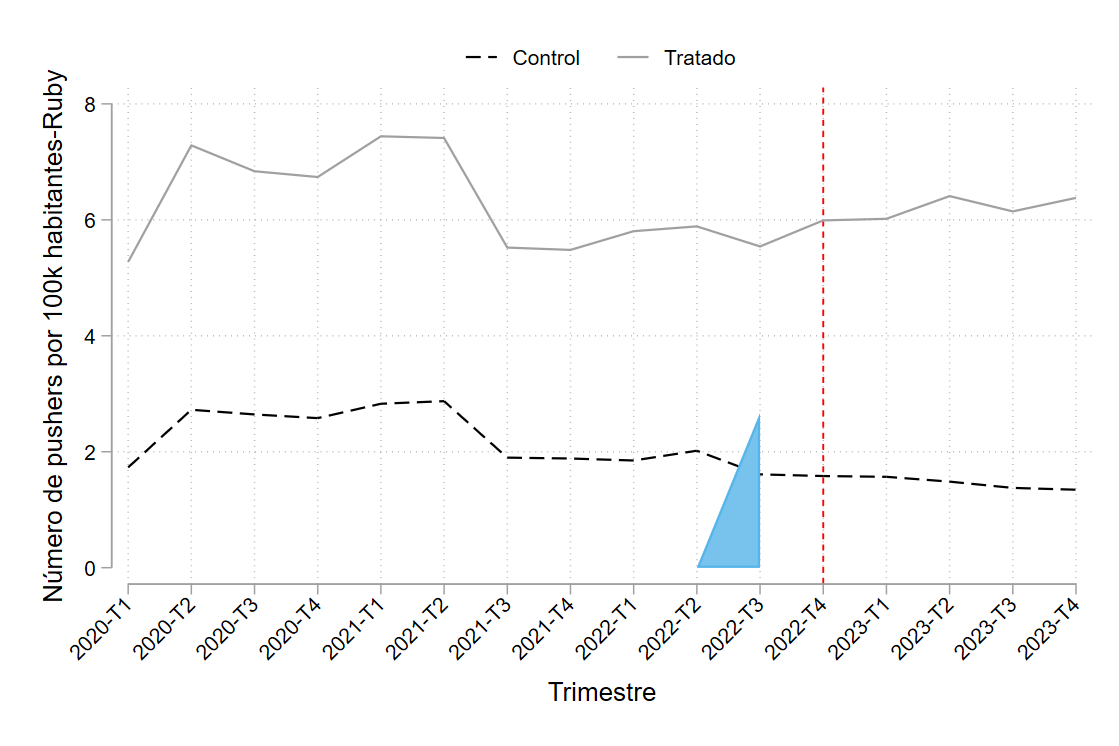
\includegraphics[width=\textwidth]{Rubysdid_trends12.png}
  \caption*{(e)–(f) SDiD}
\end{subfigure}
\caption{Tendencias y ponderaciones estimadas de Ruby \textit{unique pushers} por cada 100 mil personas}
\label{fig:figura11}
\end{figure}

\begin{figure}[htbp]
\centering
\begin{subfigure}{\textwidth}\centering
  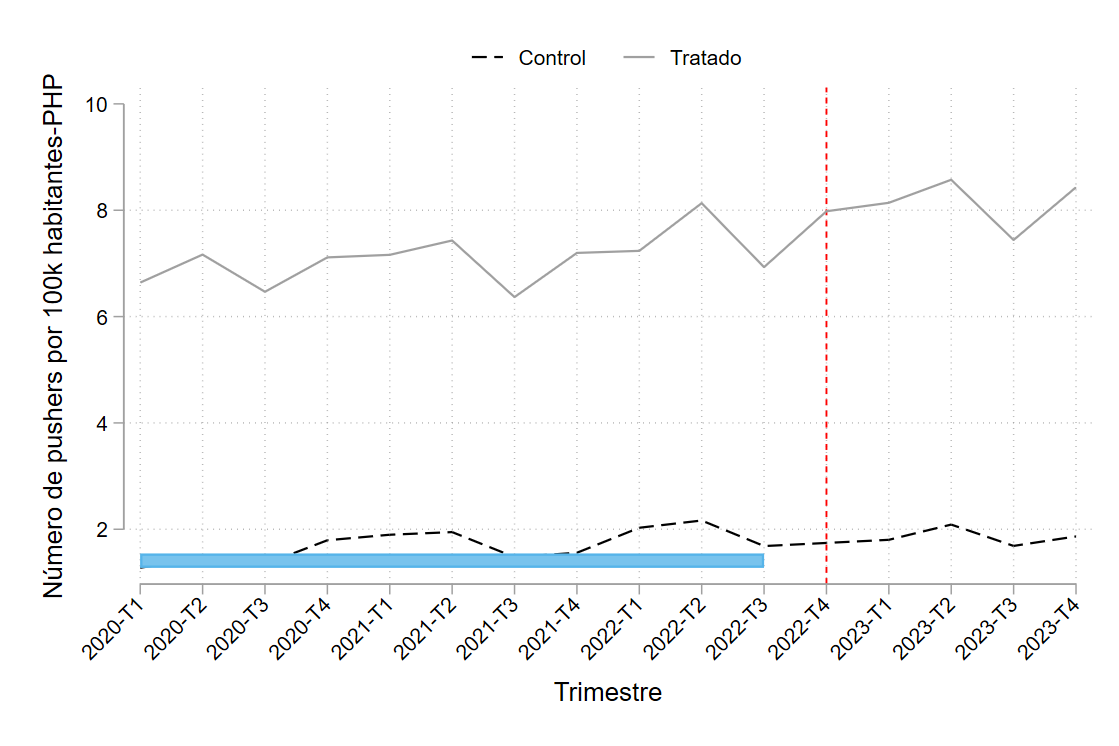
\includegraphics[width=\textwidth]{PHPdid_trends12.png}
  \caption*{(a)–(b) DiD}
\end{subfigure}\\[6pt]
\begin{subfigure}{\textwidth}\centering
  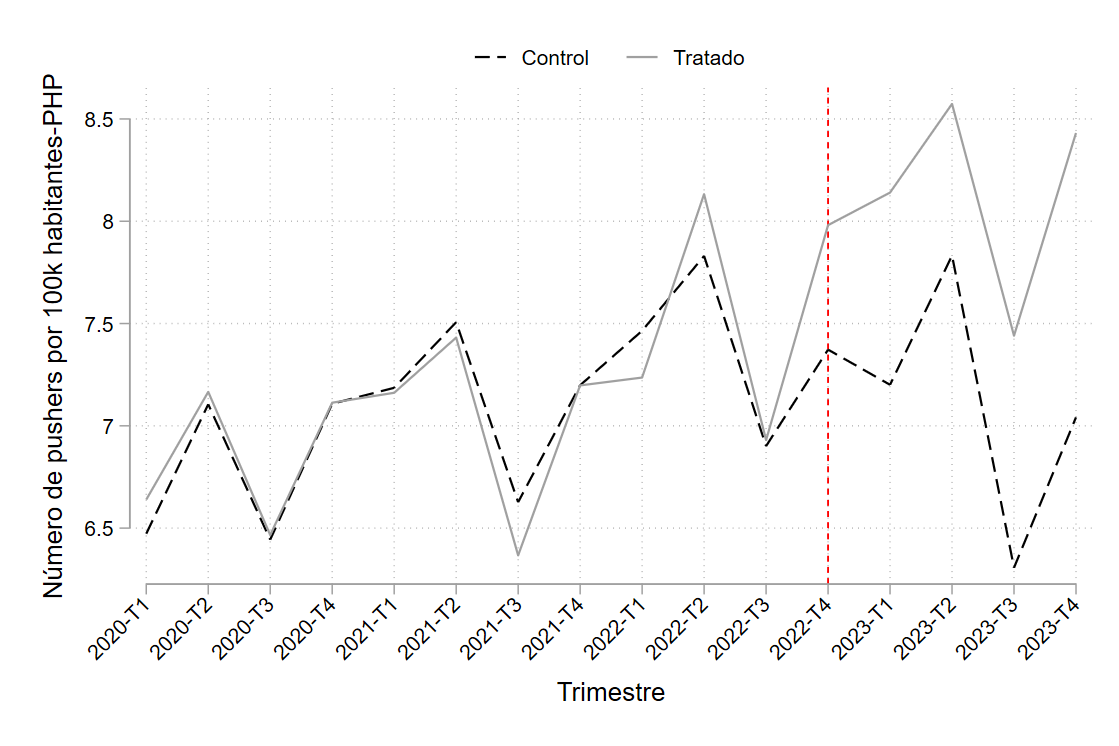
\includegraphics[width=\textwidth]{PHPsc_trends12.png}
  \caption*{(c)–(d) SC}
\end{subfigure}\\[6pt]
\begin{subfigure}{\textwidth}\centering
  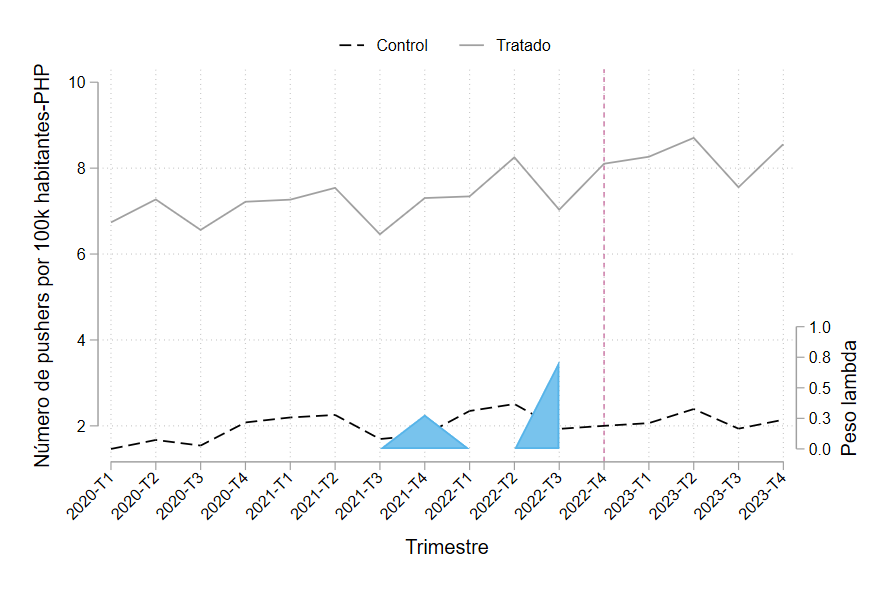
\includegraphics[width=\textwidth]{PHPsdid_trends12.png}
  \caption*{(e)–(f) SDiD}
\end{subfigure}
\caption{Tendencias y ponderaciones estimadas de PHP \textit{unique pushers} por cada 100 mil personas}
\label{fig:figura12}
\end{figure}

\begin{figure}[htbp]
\centering
\begin{subfigure}{\textwidth}\centering
  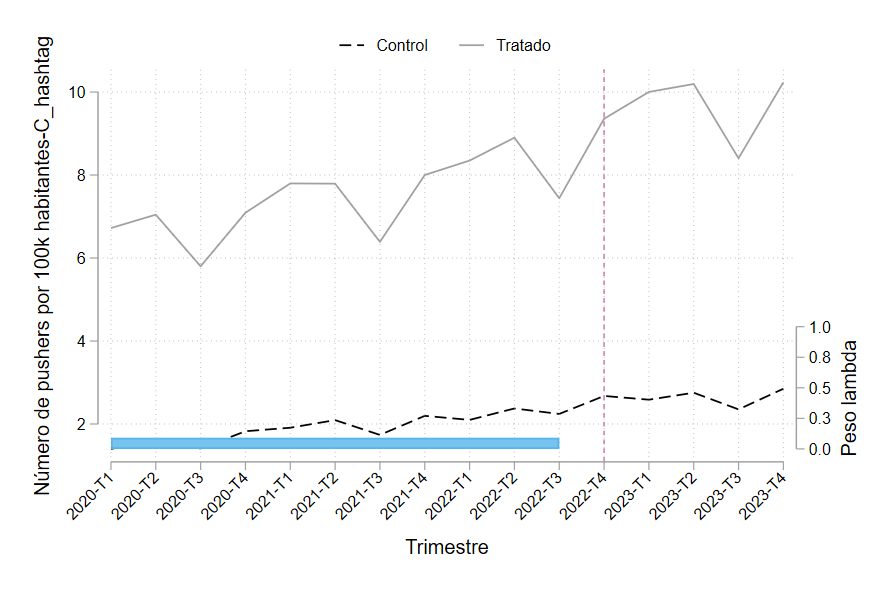
\includegraphics[width=\textwidth]{C_hashtagdid_trends12.png}
  \caption*{(a)–(b) DiD}
\end{subfigure}\\[6pt]
\begin{subfigure}{\textwidth}\centering
  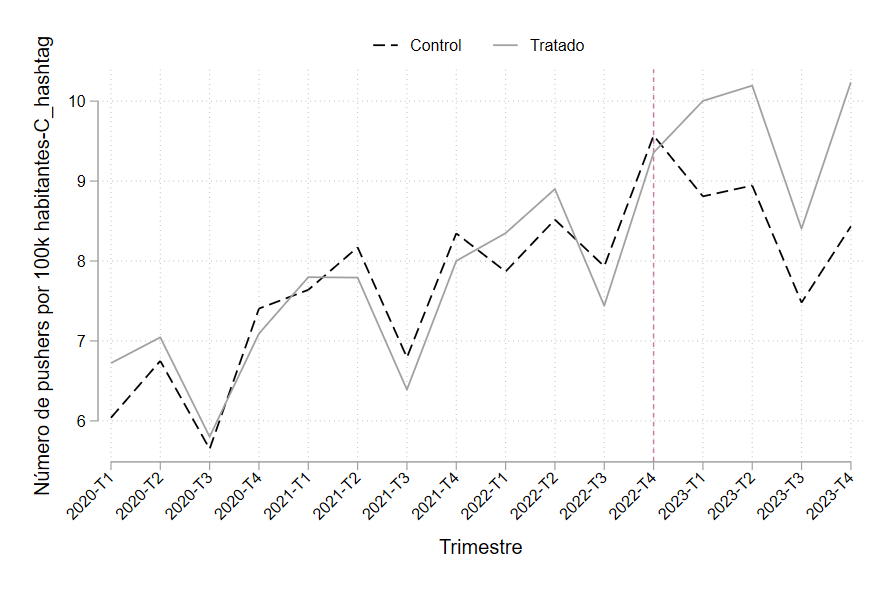
\includegraphics[width=\textwidth]{C_hashtagsc_trends12.png}
  \caption*{(c)–(d) SC}
\end{subfigure}\\[6pt]
\begin{subfigure}{\textwidth}\centering
  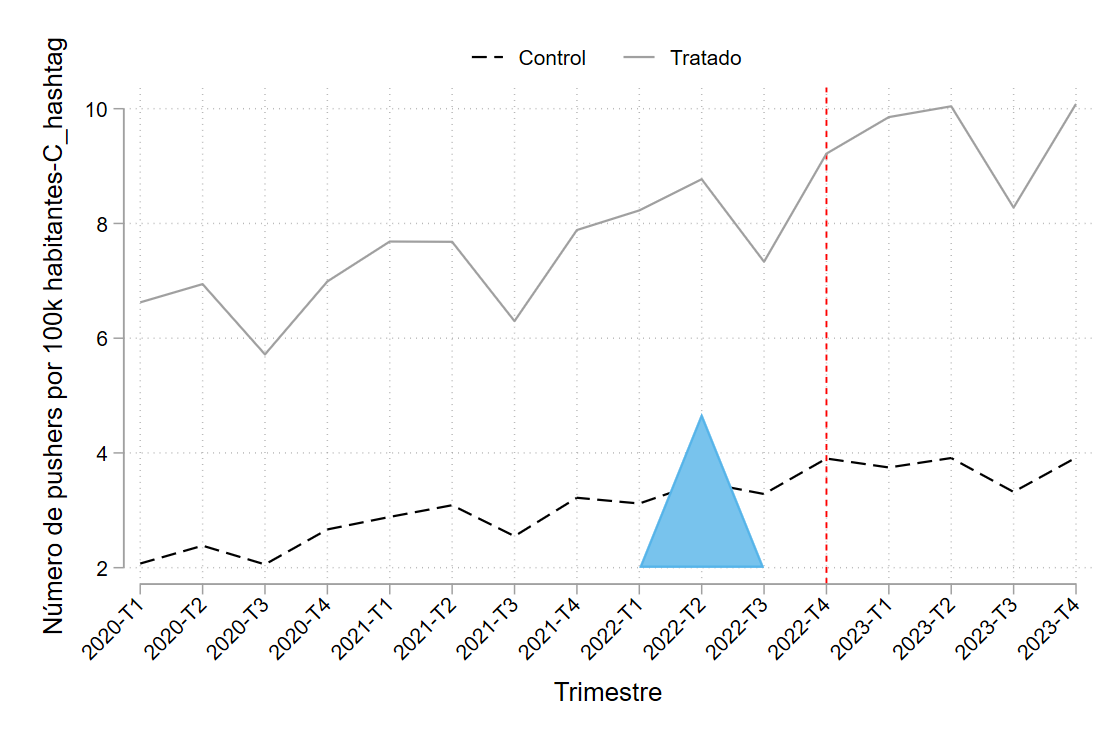
\includegraphics[width=\textwidth]{C_hashtagsdid_trends12.png}
  \caption*{(e)–(f) SDiD}
\end{subfigure}
\caption{Tendencias y ponderaciones estimadas de C\# \textit{unique pushers} por cada 100 mil personas}
\label{fig:figura13}
\end{figure}

\begin{figure}[htbp]
\centering
\begin{subfigure}{\textwidth}\centering
  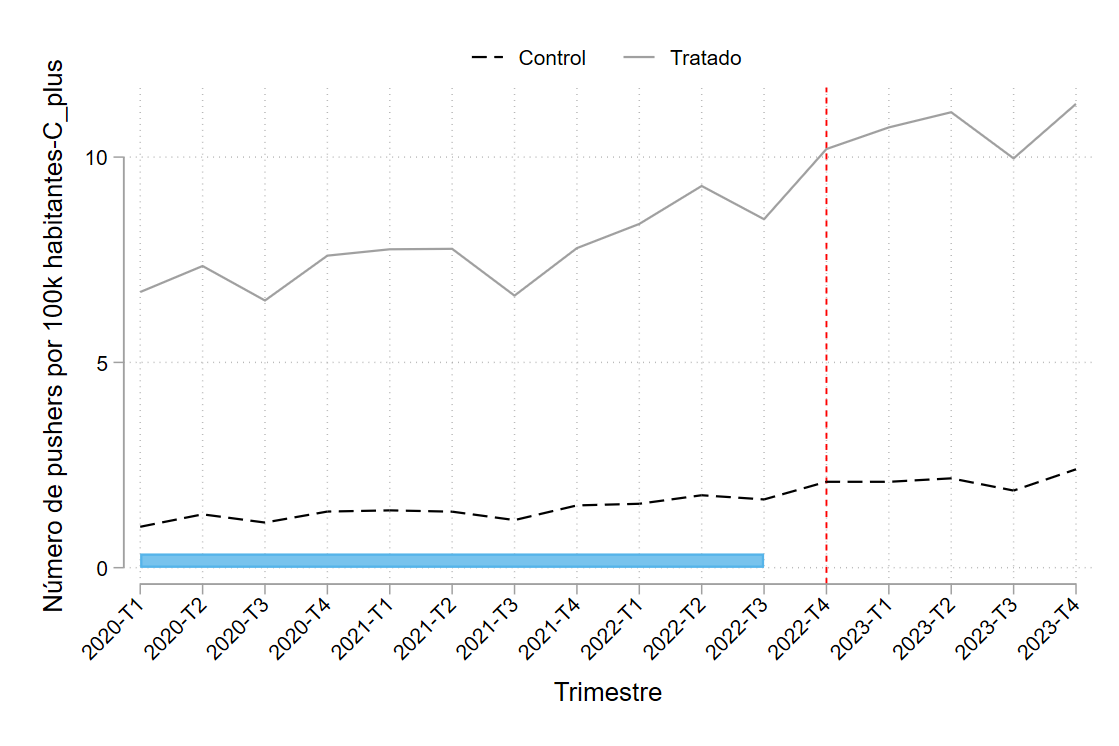
\includegraphics[width=\textwidth]{C_plusdid_trends12.png}
  \caption*{(a)–(b) DiD}
\end{subfigure}\\[6pt]
\begin{subfigure}{\textwidth}\centering
  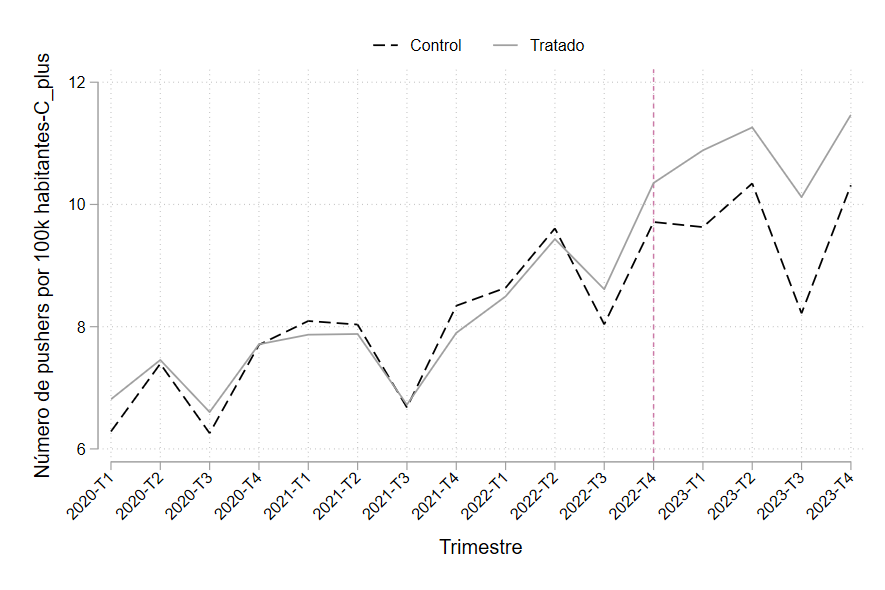
\includegraphics[width=\textwidth]{C_plussc_trends12.png}
  \caption*{(c)–(d) SC}
\end{subfigure}\\[6pt]
\begin{subfigure}{\textwidth}\centering
  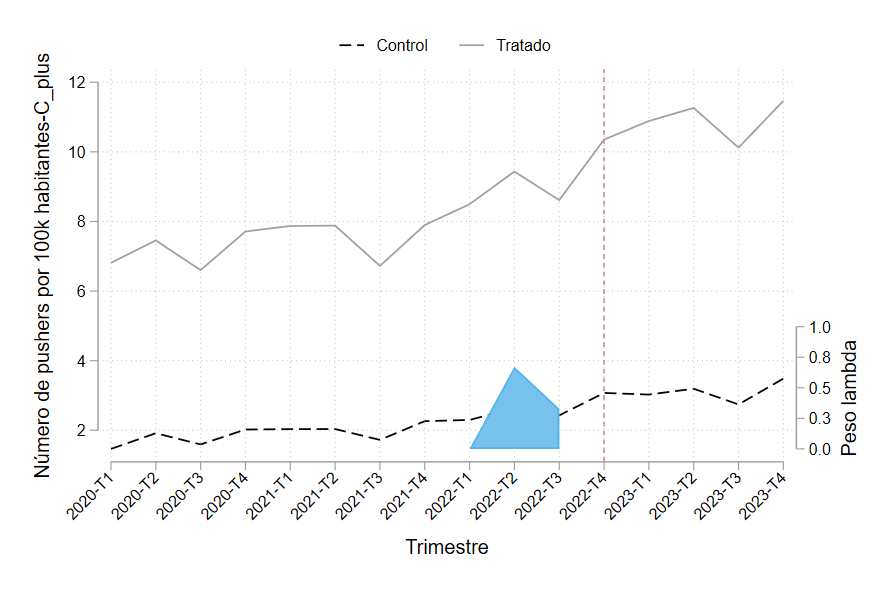
\includegraphics[width=\textwidth]{C_plussdid_trends12.png}
  \caption*{(e)–(f) SDiD}
\end{subfigure}
\caption{Tendencias y ponderaciones estimadas de C++ \textit{unique pushers} por cada 100 mil personas}
\label{fig:figura14}
\end{figure}

\begin{figure}[htbp]
\centering
\begin{subfigure}{\textwidth}\centering
  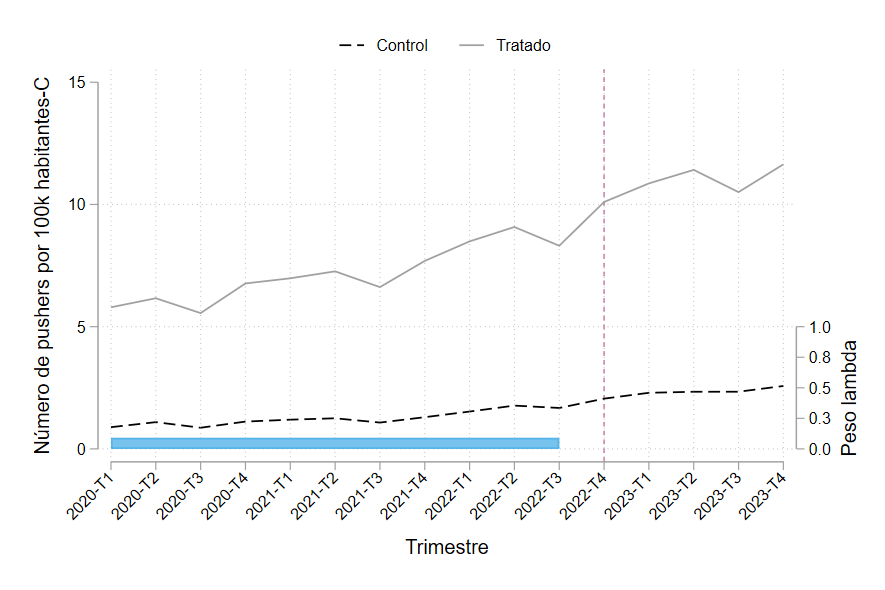
\includegraphics[width=\textwidth]{Cdid_trends12.png}
  \caption*{(a)–(b) DiD}
\end{subfigure}\\[6pt]
\begin{subfigure}{\textwidth}\centering
  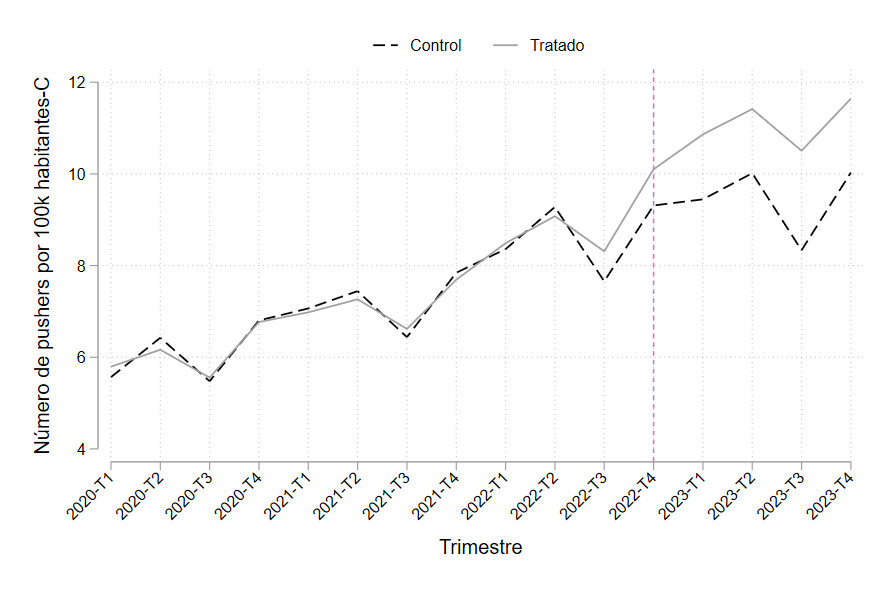
\includegraphics[width=\textwidth]{Csc_trends12.png}
  \caption*{(c)–(d) SC}
\end{subfigure}\\[6pt]
\begin{subfigure}{\textwidth}\centering
  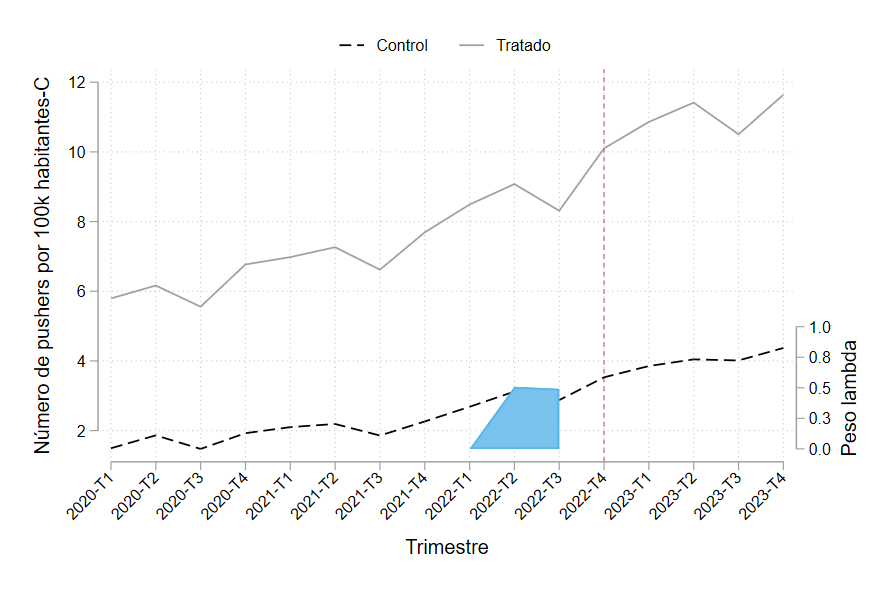
\includegraphics[width=\textwidth]{Csdid_trends12.png}
  \caption*{(e)–(f) SDiD}
\end{subfigure}
\caption{Tendencias y ponderaciones estimadas de C \textit{unique pushers} por cada 100 mil personas}
\label{fig:figura15}
\end{figure}


\section{Anexos}

\subsection*{Anexo 1: Disponibilidad global de ChatGPT}
\textit{Listado de países según la disponibilidad de acceso al servicio de ChatGPT}

\begin{figure}[htbp]
\centering
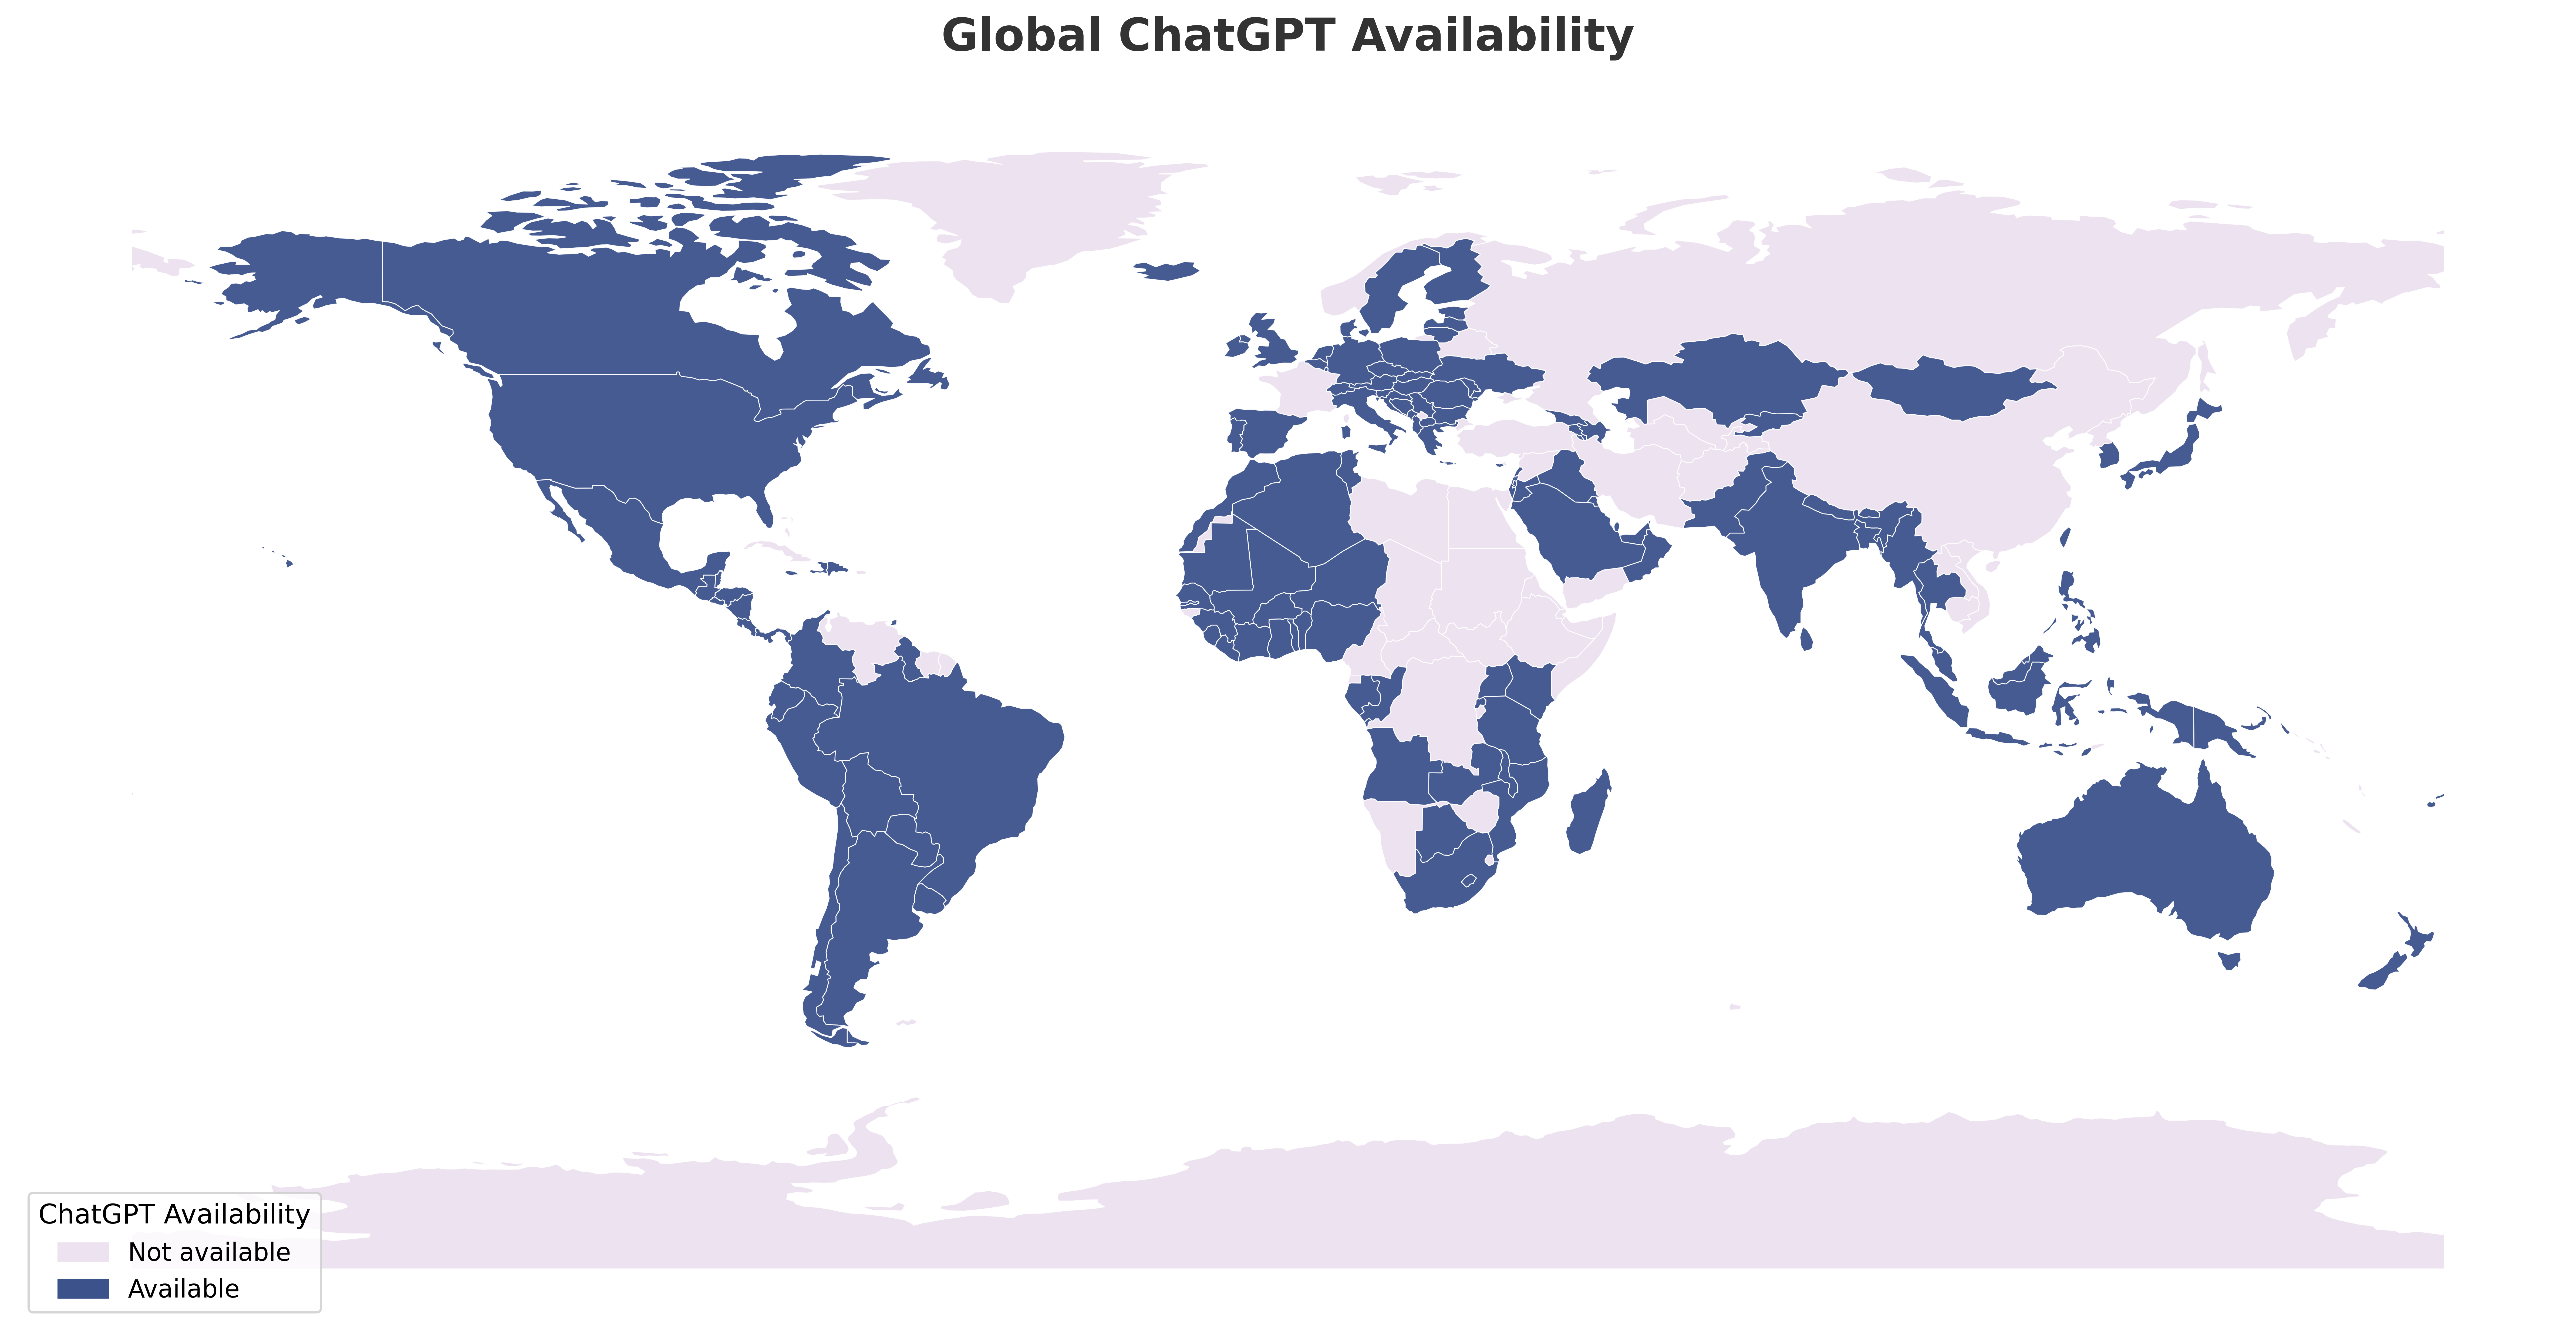
\includegraphics[width=\textwidth]{chatgpt_global_availability_map.png}
\caption{Mapa de disponibilidad global de ChatGPT}
\label{fig:mapa_gpt}
\end{figure}



\begin{table}[htbp]
\centering
\begin{tabular}{lccc}
\toprule
ISO2 & País con GPT & ISO2 & País sin GPT \\
\midrule
AL & Albania & AF & Afghanistan \\
DZ & Algeria & BH & Bahrain \\
AD & Andorra & BY & Belarus \\
AO & Angola & BI & Burundi \\
AR & Argentina & KH & Cambodia \\
AM & Armenia & CM & Cameroon \\
AU & Australia & CN & China \\
AT & Austria & CD & Congo, The Democratic Republic of the \\
AZ & Azerbaijan & CU & Cuba \\
BD & Bangladesh & EG & Egypt \\
BB & Barbados & SZ & Eswatini \\
BE & Belgium & ET & Ethiopia \\
BZ & Belize & GP & Guadeloupe \\
BJ & Benin & HK & Hong Kong \\
BT & Bhutan & IR & Iran, Islamic Republic of \\
BO & Bolivia, Plurinational State of & LA & Lao People's Democratic Republic \\
BA & Bosnia and Herzegovina & LY & Libya \\
BW & Botswana & MO & Macao \\
BR & Brazil & PR & Puerto Rico \\
BN & Brunei Darussalam & RU & Russian Federation \\
BG & Bulgaria & RE & Réunion \\
BF & Burkina Faso & SO & Somalia \\
CV & Cabo Verde & SD & Sudan \\
CA & Canada & SY & Syrian Arab Republic \\
CL & Chile & TJ & Tajikistan \\
CO & Colombia & TM & Turkmenistan \\
CG & Congo & TR & Türkiye \\
CR & Costa Rica & UZ & Uzbekistan \\
HR & Croatia & VE & Venezuela, Bolivarian Republic of \\
CY & Cyprus & VN & Viet Nam \\
CZ & Czechia & YE & Yemen \\
CI & Côte d'Ivoire & ZW & Zimbabwe \\
DK & Denmark &  &  \\
DO & Dominican Republic &  &  \\
EC & Ecuador &  &  \\
SV & El Salvador &  &  \\
EE & Estonia &  &  \\
FI & Finland &  &  \\
FR & France &  &  \\
GA & Gabon &  &  \\
GM & Gambia &  &  \\
GE & Georgia &  &  \\
DE & Germany &  &  \\
GH & Ghana &  &  \\
GR & Greece &  &  \\
GT & Guatemala &  &  \\
GN & Guinea &  &  \\
HT & Haiti &  &  \\
HN & Honduras &  &  \\
HU & Hungary &  &  \\
IS & Iceland &  &  \\
IN & India &  &  \\
ID & Indonesia &  &  \\
IQ & Iraq &  &  \\
IE & Ireland &  &  \\
IL & Israel &  &  \\
IT & Italy &  &  \\
JM & Jamaica &  &  \\
JP & Japan &  &  \\
JO & Jordan &  &  \\
KZ & Kazakhstan &  &  \\
KE & Kenya &  &  \\
KR & Korea, Republic of &  &  \\
KW & Kuwait &  &  \\
KG & Kyrgyzstan &  &  \\
LV & Latvia &  &  \\
LB & Lebanon &  &  \\
LS & Lesotho &  &  \\
LR & Liberia &  &  \\
LT & Lithuania &  &  \\
LU & Luxembourg &  &  \\
MG & Madagascar &  &  \\
MW & Malawi &  &  \\
MY & Malaysia &  &  \\
MV & Maldives &  &  \\
ML & Mali &  &  \\
MT & Malta &  &  \\
MR & Mauritania &  &  \\
MU & Mauritius &  &  \\
MX & Mexico &  &  \\
MD & Moldova, Republic of &  &  \\
MN & Mongolia &  &  \\
ME & Montenegro &  &  \\
MA & Morocco &  &  \\
MZ & Mozambique &  &  \\
MM & Myanmar &  &  \\
NP & Nepal &  &  \\
NL & Netherlands &  &  \\
NZ & New Zealand &  &  \\
NI & Nicaragua &  &  \\
NE & Niger &  &  \\
NG & Nigeria &  &  \\
MK & North Macedonia &  &  \\
NO & Norway &  &  \\
OM & Oman &  &  \\
PK & Pakistan &  &  \\
PS & Palestine, State of &  &  \\
PA & Panama &  &  \\
PG & Papua New Guinea &  &  \\
PY & Paraguay &  &  \\
PE & Peru &  &  \\
PH & Philippines &  &  \\
PL & Poland &  &  \\
PT & Portugal &  &  \\
QA & Qatar &  &  \\
RO & Romania &  &  \\
RW & Rwanda &  &  \\
SA & Saudi Arabia &  &  \\
SN & Senegal &  &  \\
RS & Serbia &  &  \\
SC & Seychelles &  &  \\
SL & Sierra Leone &  &  \\
SG & Singapore &  &  \\
SK & Slovakia &  &  \\
SI & Slovenia &  &  \\
ZA & South Africa &  &  \\
ES & Spain &  &  \\
LK & Sri Lanka &  &  \\
SE & Sweden &  &  \\
CH & Switzerland &  &  \\
TW & Taiwan, Province of China &  &  \\
TZ & Tanzania, United Republic of &  &  \\
TH & Thailand &  &  \\
TG & Togo &  &  \\
TT & Trinidad and Tobago &  &  \\
TN & Tunisia &  &  \\
UG & Uganda &  &  \\
UA & Ukraine &  &  \\
AE & United Arab Emirates &  &  \\
GB & United Kingdom &  &  \\
US & United States &  &  \\
UY & Uruguay &  &  \\
ZM & Zambia &  &  \\
\bottomrule
\end{tabular}
\end{table}


\textbf{ANEXO 2}\\
\textbf{Justificación de la no inclusión de variables de control}\\
En el presente estudio, no se incorporaron variables de control adicionales en las estimaciones realizadas mediante los métodos Difference-in-Differences (DID), Synthetic Control (SC) y Synthetic Difference-in-Differences (SDID). Esta decisión se fundamenta principalmente en la limitada disponibilidad de variables comparables para todos los países incluidos en el análisis. Si bien existen diversas bases de datos internacionales con información potencialmente relevante, como las del Banco Mundial, muchas de ellas no ofrecen una cobertura completa o no son compatibles con la estructura de panel utilizada en esta investigación. La base de datos empleada se encuentra organizada en forma de un panel consistente para un conjunto específico de países y periodos, y al realizar el proceso de imputación para pasar de datos trimestrales a datos anuales, el número de observaciones se redujo de 26 400 a 6 600. Adicionalmente, la incorporación de variables provenientes de fuentes externas implicó nuevas pérdidas de muestras debido a valores faltantes, lo que redujo aún más la muestra disponible. Como se muestra en las dos primeras tablas, inicialmente se produjo la eliminación de tres países (dos pertenecientes al grupo de control y uno al grupo tratado), y posteriormente la presencia de valores vacíos en las variables adicionales generó una reducción aproximada de 340 observaciones adicionales, provocando además un desbalance entre los grupos de tratamiento y control. Esta reducción en el número de unidades disponibles compromete la estabilidad y validez de las estimaciones, especialmente en los métodos SC y SDID, los cuales requieren un conjunto amplio y depurado de países comparables para construir un contrafactual válido.



\textit{Mapeo de}\textit{ la cantidad de}\textit{ muestras}



\begin{table}[htbp]
\centering
\begin{tabular}{lc}
\toprule
Tipo & Cantidad \\
\midrule
Quarter & 26400 \\
Year & 6600 \\
Final & 6480 \\
\bottomrule
\end{tabular}
\end{table}


\textit{C}\textit{omparación por grupo}\textit{ de muestras}



\begin{table}[htbp]
\centering
\begin{tabular}{lcccc}
\toprule
group & quarter\_samples & year\_samples & final\_samples & lost\_q\_to\_y \\
\midrule
0 & 5120 & 1280 & 1200 & 3840 \\
1 & 21280 & 5320 & 5280 & 15960 \\
\bottomrule
\end{tabular}
\end{table}


\textit{Países}\textit{eliminados}



\begin{table}[htbp]
\centering
\begin{tabular}{lc}
\toprule
iso2\_code & gpt\_available \\
\midrule
GF & 0 \\
RE & 0 \\
TW & 1 \\
\bottomrule
\end{tabular}
\end{table}


\textit{Missing}\textit{values}\textit{o datos vacíos }\textit{por }\textit{país}



\begin{table}[htbp]
\centering
\begin{tabular}{lcc}
\toprule
iso2\_code & gpt\_available\_country & n\_rows\_missing \\
\midrule
ET & 0 & 20 \\
HT & 1 & 40 \\
IN & 1 & 20 \\
KE & 1 & 30 \\
PG & 1 & 10 \\
PR & 0 & 20 \\
SD & 0 & 30 \\
SO & 0 & 20 \\
SY & 0 & 40 \\
TM & 0 & 40 \\
VE & 0 & 40 \\
YE & 0 & 30 \\
\bottomrule
\end{tabular}
\end{table}


% Tabla controles — generada por Stata (Section 6 de all_code.py)
\begin{table}[htbp]\centering
\caption{Impacto de ChatGPT en el n\'{u}mero de programadores (con controles)}
\label{tab:tabla4}
\begin{threeparttable}
{\def\sym#1{\ifmmode^{#1}\else\(^{#1}\)\fi}
\begin{tabular}{lccccc}
\toprule
Lenguaje & DID & SC & SDID & Obs. & \shortstack{Baseline \\ Mean} \\
\midrule
C & 2.774*** & 1.433 & 1.396*** & 2544 & 6.232 \\
              & (0.367) & (1.240) & (0.424) & & \\
\addlinespace
C\# & 1.475*** & 1.049 & 0.422 & 2544 & 6.557 \\
              & (0.383) & (1.252) & (0.386) & & \\
\addlinespace
C++ & 2.236*** & 1.242 & 1.157*** & 2544 & 6.807 \\
              & (0.419) & (0.979) & (0.437) & & \\
\addlinespace
Go & 1.411*** & 0.689 & 0.728*** & 2544 & 2.230 \\
              & (0.176) & (0.606) & (0.270) & & \\
\addlinespace
Java & 2.831*** & 2.224 & 1.726** & 2544 & 11.467 \\
              & (0.832) & (2.038) & (0.874) & & \\
\addlinespace
JavaScript & 14.106*** & 10.470** & 9.142*** & 2544 & 36.571 \\
              & (2.856) & (4.738) & (3.228) & & \\
\addlinespace
PHP & 0.994* & 0.974 & 1.034** & 2544 & 6.381 \\
              & (0.523) & (1.029) & (0.470) & & \\
\addlinespace
Python & 7.831*** & 2.028 & 4.700*** & 2544 & 20.003 \\
              & (1.147) & (3.531) & (1.324) & & \\
\addlinespace
Ruby & 0.312 & 1.605* & 0.864*** & 2544 & 5.592 \\
              & (0.272) & (0.855) & (0.278) & & \\
\addlinespace
TypeScript & 7.189*** & 2.742 & 3.058*** & 2544 & 8.571 \\
              & (0.846) & (2.244) & (0.870) & & \\
\addlinespace
\bottomrule
\end{tabular}}
\begin{tablenotes}
\footnotesize
\item \textit{Nota.} Estimaciones del efecto promedio del tratamiento (ATT) del acceso a ChatGPT sobre el n\'{u}mero de \textit{unique pushers} por cada 100\,000 habitantes. Las columnas DID, SC y SDID corresponden a Diferencias en Diferencias, Control Sint\'{e}tico (Abadie et al., 2010) y Diferencias en Diferencias Sint\'{e}tica (Arkhangelsky et al., 2021), respectivamente, todos estimados mediante la librer\'{i}a \texttt{synthdid} de Python (Clarke et al., 2023). Se incluyen como variables de control el porcentaje de individuos que usan computadora y el porcentaje que usa internet, extra\'{i}das del Banco Mundial, incorporadas mediante un \textit{partial-out} de efectos fijos de unidad y tiempo. Los errores est\'{a}ndar se obtienen por \textit{bootstrap}: 100 replicaciones para DiD y SDiD; 2\,000 replicaciones para SC (cuya optimizaci\'{o}n cuadr\'{a}tica introduce mayor variabilidad muestral por iteraci\'{o}n). El periodo de tratamiento inicia en Q4-2022. Fuentes: GitHub Innovation Graph (\url{https://github.com/github/innovationgraph}); Banco Mundial, Indicadores de Desarrollo Mundial. Elaboraci\'{o}n propia. Errores est\'{a}ndar entre par\'{e}ntesis. * p<0.10, ** p<0.05, *** p<0.01
\end{tablenotes}
\end{threeparttable}
\end{table}


% ── Referencias bibliográficas ────────────────────────────────────────────────

\phantomsection
\addcontentsline{toc}{section}{Referencias bibliográficas}
\begin{thebibliography}{}

\bibitem{abadie2010}
Abadie, A., Diamond, A., \& Hainmueller, A. J. (2010). Synthetic Control Methods for Comparative Case Studies: Estimating the Effect of California's Tobacco Control Program. \textit{Journal of the American Statistical Association, 105}(490), 493–505. \url{https://doi.org/10.1198/JASA.2009.AP08746}

\bibitem{abujaber2023}
Abu Jaber, M., Beganovic, A., \& Abd Almisreb, A. (2023). Methods and Applications of ChatGPT in Software Development: A Literature Review. \textit{Southeast Europe Journal of Soft Computing, 12}(1), 08–12. \url{https://www.researchgate.net/publication/370872615_Methods_and_Applications_of_ChatGPT_in_Software_Development_A_Literature_Review}

\bibitem{alshami2023}
Alshami, A., Elsayed, M., Ali, E., Eltoukhy, A. E. E., \& Zayed, T. (2023). Harnessing the Power of ChatGPT for Automating Systematic Review Process: Methodology, Case Study, Limitations, and Future Directions. \textit{Systems, 11}(7), 351. \url{https://doi.org/10.3390/SYSTEMS11070351/S1}

\bibitem{arkhangelsky2021}
Arkhangelsky, D., Athey, S., Hirshberg, D. A., Imbens, G. W., \& Wager, S. (2021). Synthetic Difference-in-Differences. \textit{American Economic Review, 111}(12), 4088–4118. \url{https://doi.org/10.1257/AER.20190159}

\bibitem{bbcmundo2023}
BBC News Mundo. (2023, marzo 31). \textit{ChatGPT: Italia se convierte en el primer país occidental en bloquear el acceso al programa de inteligencia artificial}. BBC News Mundo. \url{https://www.bbc.com/mundo/noticias-65142505}

\bibitem{brynjolfsson2023}
Brynjolfsson, W., Li, D., Raymond, L., Nber, S., Acemoglu, D., Autor, D., Axelrod, A., Dillon, E., Enam, Z., Garicano, L., Frankel, A., Manning, S., Mullainathan, S., Pierson, E., Stern, S., Rambachan, A., Reenen, J. Van, Sadun, R., Shaw, K., \& Thrun, S. (2023). Generative AI at Work. \textit{SSRN Electronic Journal}. \url{https://doi.org/10.2139/ssrn.4426942}

\bibitem{buscemi2023}
Buscemi, A. (2023). A Comparative Study of Code Generation using ChatGPT 3.5 across 10 Programming Languages. \textit{arXiv preprint arXiv:2308.04477}. \url{https://arxiv.org/abs/2308.04477}

\bibitem{chai2024}
Chai, Z., Wang, S., Liang, J., Liu, Y., Guo, H., Tian, R., Zhang, N., Zan, D., Dou, S., Huang, Y., Gao, J., Yu, D., Liu, J., Li, G., Yu, J., \& Liu, Z. (2024). McEval: Massively Multilingual Code Evaluation. \textit{arXiv preprint arXiv:2406.07436}. \url{https://arxiv.org/abs/2406.07436}

\bibitem{chui2023}
Chui, M., Hazan, E., Roberts, R., Singla, A., Smaje, K., Sukharevsky, A., Yee, L., \& Zemmel, R. (2023). The Impact of AI on Developer Productivity: Evidence from GitHub Copilot. \url{http://arxiv.org/abs/2302.06590}

\bibitem{clarke2023}
Clarke, D., Pailañir, D., Carleton Athey, S., \& Imbens, G. W. (2023). Synthetic Difference In Differences Estimation. \textit{SSRN Electronic Journal}. \url{https://doi.org/10.2139/ssrn.4346540}

\bibitem{coursera2024}
Coursera Staff. (2024). Most Popular Programming Languages in 2024 | Coursera. \textit{Coursera}. \url{https://www.coursera.org/articles/popular-programming-languages}

\bibitem{datacamp2023}
Data Camp. (2023). Top programming languages for data scientists in 2023 | DataCamp. \textit{Datacamp}. \url{https://www.datacamp.com/blog/top-programming-languages-for-data-scientists-in-2022}

\bibitem{delriochanona2023}
Del Rio-Chanona, M., Laurentsyeva, N., \& Wachs, J. (2023). Are Large Language Models a Threat to Digital Public Goods? Evidence from Activity on Stack Overflow. \url{https://arxiv.org/abs/2307.07367v1}

\bibitem{demirci2023}
Demirci, O., Hannane, J., \& Zhu, X. (2023). Who Is AI Replacing? The Impact of Generative AI on Online Freelancing Platforms. \textit{SSRN Electronic Journal}. \url{https://doi.org/10.2139/SSRN.4602944}

\bibitem{gallea2023}
Gallea, Q. (2023). From Mundane to Meaningful: AI's Influence on Work Dynamics -- evidence from ChatGPT and Stack Overflow. \url{https://arxiv.org/abs/2308.11302v1}

\bibitem{hui2023}
Hui, X., Reshef, O., \& Zhou, L. (2023). The Short-Term Effects of Generative Artificial Intelligence on Employment: Evidence from an Online Labor Market. \textit{SSRN Electronic Journal}. \url{https://doi.org/10.2139/SSRN.4527336}

\bibitem{ijaz2023}
Ijaz, S. (2023, julio 6). \textit{15 Countries That Banned ChatGPT}. Insider Monkey. \url{https://www.insidermonkey.com/blog/15-countries-that-banned-chatgpt-1165549/}

\bibitem{kalla2023}
Kalla, D., Smith, N., Samaah, F., \& Kuraku, S. (2023). Study and Analysis of Chat GPT and its Impact on Different Fields of Study. \url{https://papers.ssrn.com/abstract=4402499}

\bibitem{kreitmeir2023}
Kreitmeir, D., \& Raschky, P. A. (2023). The Unintended Consequences of Censoring Digital Technology: Evidence from Italy's ChatGPT Ban. \textit{arXiv preprint arXiv:2304.09339}. \url{https://arxiv.org/abs/2304.09339}

\bibitem{li2024}
Li, M., \& Krishnamachari, B. (2024). Evaluating ChatGPT-3.5 efficiency in solving coding problems of different complexity levels: An empirical analysis. \textit{arXiv preprint arXiv:2411.07529}. \url{https://doi.org/10.48550/arXiv.2411.07529}

\bibitem{liu2023}
Liu, J., Foster, M. G., Nan, X., Li, Y., \& Tan, Y. (2023). "Generate" the Future of Work through AI: Empirical Evidence from Online Labor Markets. \textit{SSRN Electronic Journal}. \url{https://doi.org/10.2139/ssrn.4529739}

\bibitem{Maes2025}
Maes, S. H. (2025). Ensuring the maintainability and supportability of ``vibe-coded'' software systems: A framework for bridging intuition and engineering rigor. \url{https://www.researchgate.net/profile/Stephane-Maes-2}

\bibitem{martinez2023}
Martinez, J. (2023). Guerra abierta contra ChatGPT: estos son los países que ya lo han prohibido. \textit{ABC}. \url{https://www.abc.es/tecnologia/guerra-abierta-chatgpt-paises-prohibido-20230427200409-nt.html}

\bibitem{onu2023}
ONU. (2023). El debate de la Inteligencia Artificial en la ONU. \textit{Naciones Unidas}. \url{https://unric.org/es/el-debate-de-la-inteligencia-artificial-en-la-onu/}

\bibitem{openai2018}
OpenAI. (2018). OpenAI charter. OpenAI. \url{https://openai.com/}

\bibitem{openai2024}
OpenAI. (2024). Models - OpenAI API. \url{https://platform.openai.com/docs/models}

\bibitem{rajbhoj2024}
Rajbhoj, A., Somase, A., Kulkarni, P., \& Kulkarni, V. (2024). Accelerating Software Development Using Generative AI: ChatGPT Case Study. \textit{ACM International Conference Proceeding Series}. \url{https://doi.org/10.1145/3641399.3641403}

\bibitem{rice2023}
Rice CS. (2023). Top 12 Data Science Programming Languages | MDS@Rice. \textit{Rice University}. \url{https://csweb.rice.edu/academics/graduate-programs/online-mds/blog/programming-languages-for-data-science}

\bibitem{shen2024}
Shen, Y., Ai, X., Soosai Raj, A. G., Leo John, R. J., \& Syamkumar, M. (2024). Implications of ChatGPT for Data Science Education. \textit{SIGCSE 2024 - Proceedings of the 55th ACM Technical Symposium on Computer Science Education, 1}, 1230–1236. \url{https://doi.org/10.1145/3626252.3630874}

\bibitem{statista2023}
Statista. (2023). Software - Worldwide. Market Forecast. \url{https://www.statista.com/outlook/tmo/software/worldwide#revenue}

\bibitem{tlili2023}
Tlili, A., Shehata, B., Adarkwah, M. A., Bozkurt, A., Hickey, D. T., Huang, R., \& Agyemang, B. (2023). What if the devil is my guardian angel: ChatGPT as a case study of using chatbots in education. \textit{Smart Learning Environments, 10}(1), 1–24. \url{https://doi.org/10.1186/S40561-023-00237-X/FIGURES/13}

\bibitem{unesco2023}
UNESCO. (2023). ChatGPT and artificial intelligence in higher education: A quick start guide. United Nations Educational, Scientific and Cultural Organization (UNESCO). \url{https://unesdoc.unesco.org/ark:/48223/pf0000380455}

\bibitem{wipo2022}
World Intellectual Property Organization. (2022). World Intellectual Property Report 2022 — The Direction of Innovation. \url{https://www.wipo.int/web/world-ip-report/2022-the-direction-of-innovation}

\bibitem{wu2024}
Wu, Q., Zhuang, Q., Liu, Y., \& Han, L. (2024). Technology Shock of ChatGPT, Social Attention and Firm Value: Evidence from China. \textit{SSRN}. \url{https://doi.org/10.2139/SSRN.4739412}

\bibitem{Zhang2025}
Zhang, C., \& Magerko, B. (2025). Generative AI literacy: A comprehensive framework for literacy and responsible use. \textit{arXiv}. \url{https://arxiv.org/abs/2504.19038}

\end{thebibliography}

\end{document}
